%Przykładowy plik ułatwiający złożenie projektu dyplomowego inżynierskiego.
%UWAGA: Generowany napis na stronie tytułowej o treści PROJEKT DYPLOMOWY INŻYNIERSKI został zaproponowany przeze mnie i nie jest, póki co, potwierdzony przez władze wydziału. Przed ostatecznym oddaniem tak złożonej pracy należy upewnić się jaka powinna być treść tego napisu. W momencie gdy uzyskam informację na temat treści tego napisu, dokonam niezbędnych zmian w źródłach.

%\documentclass[eng,printmode]{mgr}
\documentclass[eng,printmode,openany,oneside]{mgr}
%opcje klasy dokumentu mgr.cls zostały opisane w dołączonej instrukcji

%poniżej deklaracje użycia pakietów, usunąć to co jest niepotrzebne
\usepackage{polski} %przydatne podczas składania dokumentów w j. polskim
%\usepackage[polish]{babel}%alternatywnie do pakietu polski, wybrać jeden z nich
\usepackage[utf8]{inputenc} %kodowanie znaków, zależne od systemu
\usepackage[T1]{fontenc} %poprawne składanie polskich czcionek


%pakiety do grafiki
\usepackage{graphicx}
\usepackage{subfigure}
\usepackage{psfrag}

%pakiety dodające dużo dodatkowych poleceń matematycznych
\usepackage{amsmath}
\usepackage{amsfonts}

%pakiety wspomagające i poprawiające składanie tabel
\usepackage{supertabular}
\usepackage{array}
\usepackage{tabularx}
\usepackage{hhline}

%pakiet wypisujący na marginesie etykiety równań i rysunków zdefiniowanych przez \label{}, chcąc wygenerować finalną wersję dokumentu wystarczy usunąć poniższą linię
%\usepackage{showlabels}

%definicje własnych poleceń
\newcommand{\R}{I\!\!R} %symbol liczb rzeczywistych, działa tylko w trybie matematycznym
\newtheorem{theorem}{Twierdzenie}[section] %nowe otoczenie do składania twierdzeń

%dane do złożenia strony tytułowej
\title{System informatyczny wspomagający planowanie spotkań biznesowych}
\engtitle{IT system supporting planning business meetings}
\author{Małgorzata Wojnarowska}
\supervisor{dr inż. Jarosław Pempera}
%\guardian{dr hab. inż. Imię Nazwisko Prof. PWr, I-6} %nie używać jeśli opiekun jest tą samą osobą co prowadzący pracę

%\date{2008} %standardowo u dołu strony tytułowej umieszczany jest bieżący rok, to polecenie pozwala wstawić dowolny rok

%poniżej jest lista kierunków i specjalności na wydziale elektroniki, należy wybrać właściwe lub dopisać jeśli nie ma odpowiednich
\field{Automatyka i Robotyka (AIR)}
\specialisation{Komputerowe systemy zarządzania \\procesami produkcyjnymi (ARS)}

\graphicspath{ {img/} }
\usepackage{float}
\usepackage{listings}
\renewcommand*{\lstlistlistingname}{Spis listingów}
\renewcommand*{\tablename}{Tabela}
\usepackage{xcolor}
\usepackage{color}
\usepackage{caption}
\usepackage{mdwlist}
\usepackage{verbatim}

\definecolor{mygreen}{HTML}{78bb6d}
\definecolor{mygray}{rgb}{0.5,0.5,0.5}
\definecolor{mymauve}{HTML}{ab5959}
\definecolor{myblue}{HTML}{5998ff}

\lstset{ %
  backgroundcolor=\color{white},   % choose the background color
  basicstyle=\scriptsize,
 % basicstyle=\footnotesize,        % size of fonts used for the code
  breaklines=true,                 % automatic line breaking only at whitespace
  %captionpos=a,                    % sets the caption-position to bottom
  commentstyle=\color{mygreen},    % comment style
  escapeinside={\%*}{*)},          % if you want to add LaTeX within your code
  keywordstyle=\color{myblue},       % keyword style
  stringstyle=\color{mymauve},     % string literal style
%  xleftmargin=.2\textwidth, xrightmargin=.2\textwidth
  morecomment=[l]{//},
  morecomment=[l]{--},
  %inputencoding=utf8,
  %extendedchars=\true,
  showstringspaces=false,
  literate=%
  {ą}{{\k{a}}}1
 {ę}{{\k{e}}}1
 {Ą}{{\k{A}}}1
 {Ę}{{\k{E}}}1
 {ś}{{\'{s}}}1
 {Ś}{{\'{S}}}1
 {ź}{{\'{z}}}1
 {Ź}{{\'{Z}}}1
 {ń}{{\'{n}}}1
 {Ń}{{\'{N}}}1
 {ć}{{\'{c}}}1
 {Ć}{{\'{C}}}1
 {ó}{{\'{o}}}1
 {Ó}{{\'{O}}}1
 {ż}{{\.{z}}}1
 {Ż}{{\.{Z}}}1
 {ł}{{\l{}}}1
 {Ł}{{\l{}}}1
}

%interlinia 1.5
\linespread{1.3} 






%tutaj zaczyna się właściwa treść dokumentu
\begin{document}

\bibliographystyle{plabbrv} %tylko gdy używamy BibTeXa, ustawia polski styl bibliografii

\maketitle %polecenie generujące stronę tytułową

\tableofcontents %spis treści

%poniżej znajduje się przykładowa treść dalszej części dokumentu, zainteresowanych zachęcam do rozszyfrowania frazy "Lorem ipsum" :)
\chapter{Wstęp}
%\addcontentsline{toc}{chapter}{Wstęp}
Niektórym ludziom wydaje się, że planowanie nie jest niezbędnym elementem życia. Tacy ludzie twierdzą, że należy żyć chwilą. I rzeczywiście, wielu rzeczy można nie planować. Jednak, kiedy mamy pracę, studia, rodzinę czy po prostu więcej innych obowiązków - bez planowania daleko nie zajdziemy, a szybko zacznie się nam wydawać, że doba jest zbyt krótka.

Szczególnie ważnym aspektem jest planowanie spotkań biznesowych. Przy kontakcie z klientem, zarówno przy dłuższej współpracy, jak i potencjalnym, nie można działać spontanicznie. Ciężko wyobrazić sobie prezesa dużej firmy, który nie miałby zaplanowanych spotkań na - co najmniej - kilka dni do przodu. Aby się w tym wszystkim nie pogubić warto mieć narzędzie, które będzie odpowiadało naszym potrzebom w stu procentach. 


Takie narzędzie jak planer czy kalendarz towarzyszy nam codziennie, szczególnie w pracy. Warto, aby taki aspekt życia jak planowanie sprawiał nam maksymalnie dużo przyjemności, a jeśli i tak nie jest to ulubione zajęcie - aby planowanie odbywało się możliwie szybko oraz intuicyjnie.


W dzisiejszych czasach ludzie coraz częściej odkładają papierowe planery na rzecz telefonu czy komputera, które zawsze mają przy sobie. Dlatego w pracy przedstawiony będzie system do planowania spotkań biznesowych, który może być używany na komputerze. Dzięki temu planowanie nie będzie wymagało dodatkowego sprzętu w plecaku czy torebce, ponieważ dostęp do systemu będziemy mieć z każdego miejsca na świecie, a podczas wyjazdów biznesowych nie będzie trzeba pamiętać o niczym więcej niż laptop.


Aby czerpać maksymalnie możliwą przyjemność z planowania zaproponuję narzędzie, które jest minimalistyczne, a także proste i intuicyjne w obsłudze. System pomoże zapanować nad czasem oraz biznesowymi obowiązkami. Stworzenie odpowiedniego planu działania to podstawa organizacji.


%\section*{Cel i zakres pracy}
\chapter{Cel i zakres pracy}
Celem pracy jest zaprojektowanie i wykonanie systemu informatycznego, który ułatwi planowanie spotkań biznesowych. System ma pozwalać na intuicyjne zarządzanie spotkaniami, a także osobistymi notatkami.

Realizację pracy podzielono na następujące etapy:
\begin{itemize}
    \item stworzenie relacyjnej bazy danych,
    \item stworzenie aplikacji do planowania i zarządzania spotkaniami,
    \item stworzenie systemu do zarządzania notatkami,
    \item wdrożenie systemu, testowanie oraz uruchomienie.
\end{itemize}

Na początku pracy zostanie przeprowadzona analiza wymagań do stworzenia systemu. Zostaną przedstawione wymagania zarówno funkcjonalne, czyli projekt funkcji systemu, a także niefunkcjonalne, takie jak użyte technologie, narzędzia czy zaprojektowane zabezpieczenia systemu.

W kolejnym etapie zostanie przedstawiony projekt bazy danych, w której będą znajdować się dane dotyczące klientów, pracowników, a także ich spotkań i notatek. Ponieważ baza danych jest relacyjna, zostaną pokazane także relacje pomiędzy poszczególnymi tabelami oraz uprawnienia grup użytkowników.

Następnie zostanie pokazany interfejs użytkownika, jego przykładowe funkcjonalności i zabezpieczenia.

W kolejnym rozdziale znajduje się implementacja baz danych, czyli stworzenie tabel, ich indeksów oraz ograniczeń. Na końcu rozdziału przedstawione jest testowanie bazy danych.

Ostatni etap pracy to implementacja i testy samej aplikacji, opis oraz programowanie wybranych funkcji systemu. 

\chapter{Wymagania projektowe}



\section{Opis działania systemu}
System jest przeznaczony dla pracowników firmy. Każdy z nich ma możliwość rejestracji i zalogowania się. Mogą dowolnie planować swoje spotkania biznesowe, a także dodawać i edytować notatki. Każde spotkanie może zostać zaplanowane na dany dzień i godzinę. Notatka może być dodana do dowolnego dnia lub bez daty, dzięki czemu można dowolnie nimi zarządzać, ułatwiając organizację spotkań. Dodatkowo w systemie jest możliwość edycji oraz usuwania notatek i spotkań, a także przeglądania ich w zależności od dnia, miesiąca i roku. Każdy pracownik może także dodać klienta do bazy danych i umówić spotkanie z każdym klientem.

\section{Wymagania funkcjonalne}
Każde spotkanie ma ustaloną datę oraz godzinę, kiedy się odbędzie. Na dany dzień można też zaplanować jakieś działanie lub dodać informację za pomocą notatki. Notatka może również nie mieć określonej daty, a być jedynie przypomnieniem. Dostęp do systemu planowania mogą mieć wyłącznie zalogowani pracownicy. Użytkownik to każda osoba, która przegląda stronę, a pracownik to każda zarejestrowana osoba.

\subsection*{Użytkownik}
System informatyczny ma dostarczyć następujące funkcjonalności dla użytkownika:


\begin{itemize}
	\item możliwość rejestracji,
	\item możliwość zalogowania,
	\item możliwość przeglądania strony głównej.
\end{itemize}


\subsection*{Pracownik}
Liczba funkcjonalności dla pracownika jest znacznie większa:






%\subsection*{Dla pracownika}
\begin{itemize}
	\item planowanie spotkania,
	\item stworzenie notatki,
	\item dodanie klienta,
	\item przeglądanie notatek i spotkań,
	\item dowolne zarządzanie notatkami i spotkaniami,
	\item możliwość zalogowania,
	\item możliwość rejestracji.
\end{itemize}




\section{Wymagania niefunkcjonalne}

Zaprojektowany system powinien być wygodny i intuicyjny w użytkowaniu dla każdego pracownika. System do planowania spotkań biznesowych ma być użyteczny oraz prosty w obsłudze. 

\subsection*{Technologie i narzędzia}
Aby stworzyć aplikację zostaną użyte różne technologie i narzędzia. Do projektu i implementacji części front-end wykorzystano HTML5 oraz CSS3 \cite{bib:3}.

Relacyjna baza danych stworzona zostanie w MySQL \cite{bib:1}, \cite{bib:2}, a następnie połączona ze stroną za pomocą PHP \cite{bib:1}, \cite{bib:2}. Back-end systemu zostanie wykonany w języku PHP.

Projekt zostanie wykonany na localhost, gdzie zostanie użyty serwer XAMPP/Apache.

Do stworzenia systemu użyte zostały następujące technologie i narzędzia:
\begin{itemize}
	\item serwer: Apache,
	\item system operacyjny: MacOS,
	\item szablon: HTML5 oraz CSS3,
	\item programowanie oraz połączenie z bazą danych: PHP,
	\item relacyjna baza danych: MySQL.
\end{itemize}

\subsection*{Bezpieczeństwo systemu}
Aby zachować maksymalne bezpieczeństwo systemu, zostaną zastosowane następujące zabezpieczenia: 
\begin{itemize}
	\item możliwość przeglądania systemu jedynie dla pracowników,
	\item szyfrowanie haseł,
	\item potwierdzenie rejestracji za pomocą wiadomości e-mail.
\end{itemize}

\subsection*{Przyjęte założenia projektowe}
Do realizacji projektu przyjęto następujące założenia projektowe:
\begin{itemize}
	\item stworzenie wygodnego systemu do planowania spotkań biznesowych,
	\item stworzenie systemu do zarządzania notatkami,
	\item system z możliwością logowania i rejestracji.
\end{itemize}

\chapter{Projekt systemu}
\section{Projekt relacyjnej bazy danych}

Baza danych spełnia podstawowe zasady projektowe, jest to baza znormalizowana. Dzięki normalizacji możemy organizować dane, tak aby ich ilość była optymalna oraz eliminować anomalie, powtarzające się dane. Atomowość danych zapewnia, że każda tabela przechowuje dane tak, aby w jednym polu znalazła się jedna informacja, np w tabeli 'Pracownicy' osobno są kolumny 'Imie' oraz 'Nazwisko'. Każda tabela przechowuje dane dotyczące tylko obiekty właściwe dla niej. W tabeli 'Spotkania' nie ma informacji o kliencie innych niż 'IdKlienta'. Resztę danych, jak imię i nazwisko można wyciągnąć już z tabeli 'Klienci'. Żadne z kolumn we wszystkich 4 tabelach nie zależą od innej kolumny w danej tabeli. Znaczy to, że baza danych jest znormalizowana do trzeciej postaci normalnej. Dane znajdujące się w bazie przechowuje się w czterech tabelach:
\begin{itemize}
	\item Klienci,
	\item Spotkania,
	\item Pracownicy,
	\item Notatki.
\end{itemize}
Tabela 'Klienci' zawiera opis klientów firmy, w szczególności imię, nazwisko, nazwę firmy, w której pracuje oraz e-mail. Połączona jest z tabelą 'Spotkania' przez unikalny klucz 'IdKlienta'. 

Tabela 'Spotkania' przechowuje dane dotyczące spotkań: opis spotkania (pole 'Tytul'), datę, godzinę praz klucze identyfikujące klienta i pracownika, którzy odbywają spotkanie. Każde spotkanie może mieć przypisanego jednego klienta oraz jednego pracownika.

Informacje dotyczące pracowników przechowywane są w tabeli 'Pracownicy', zawierają się tam takie informacje jak imię, nazwisko, stanowisko, na którym pracuje, e-mail, hasło w zaszyfrowanej postaci, login oraz unikalny indeks 'IdPracownika', który jest kluczem łączącym tabelę 'Spotkania' oraz 'Notatki'. 

Ostatnią z tabel jest tabela 'Notatki'. W tabeli oprócz samej treści notatki przechowywany jest też jej tytuł oraz data. Kluczem głównym tabeli jest 'IdNotatki'. Do każdej notatki przypisany jest tylko jeden pracownik. 

Model konceptualny struktury bazy danych przedstawiony jest na Rysunku \ref{fig:1}.


\begin{figure}[H]
	\centering
	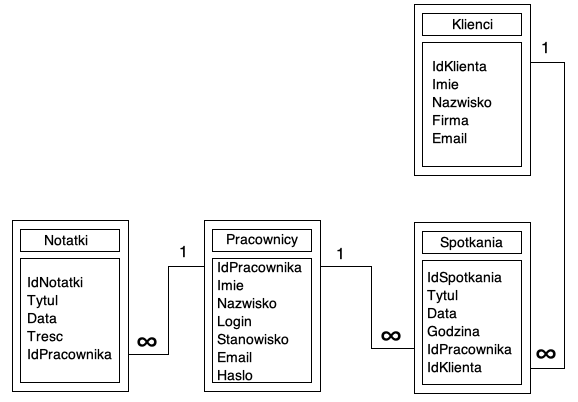
\includegraphics[width=0.75\textwidth]{model_koncept}
	\caption{Model konceptualny}
	\label{fig:1}
\end{figure}

Model fizyczny bazy danych został przedstawiony na Rysunku \ref{fig:2}. Tabele \ref{tab:1} - \ref{tab:4} przedstawiają szczegółowy opis pól poszczególnych tabel w bazie danych.

\begin{figure}[H]
	\centering
	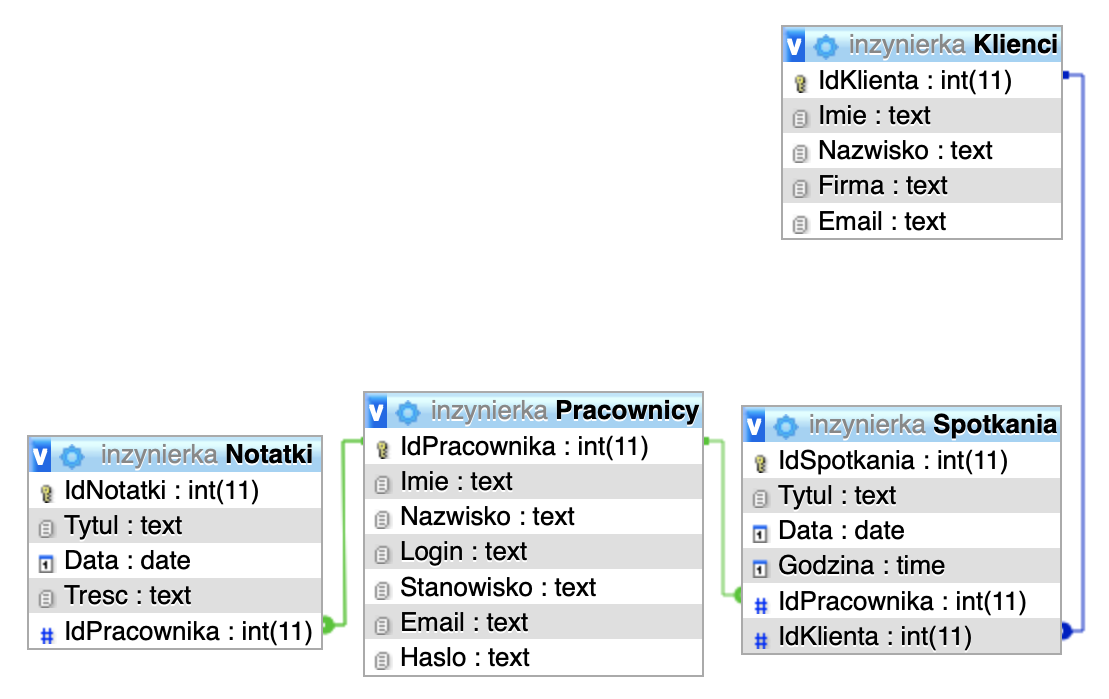
\includegraphics[width=0.75\textwidth]{model_logiczny}
	\caption{Model gotowej bazy danych}
	\label{fig:2}
\end{figure}

\begin{table}[H]
	\centering
	\caption{Tabela pracowników}
	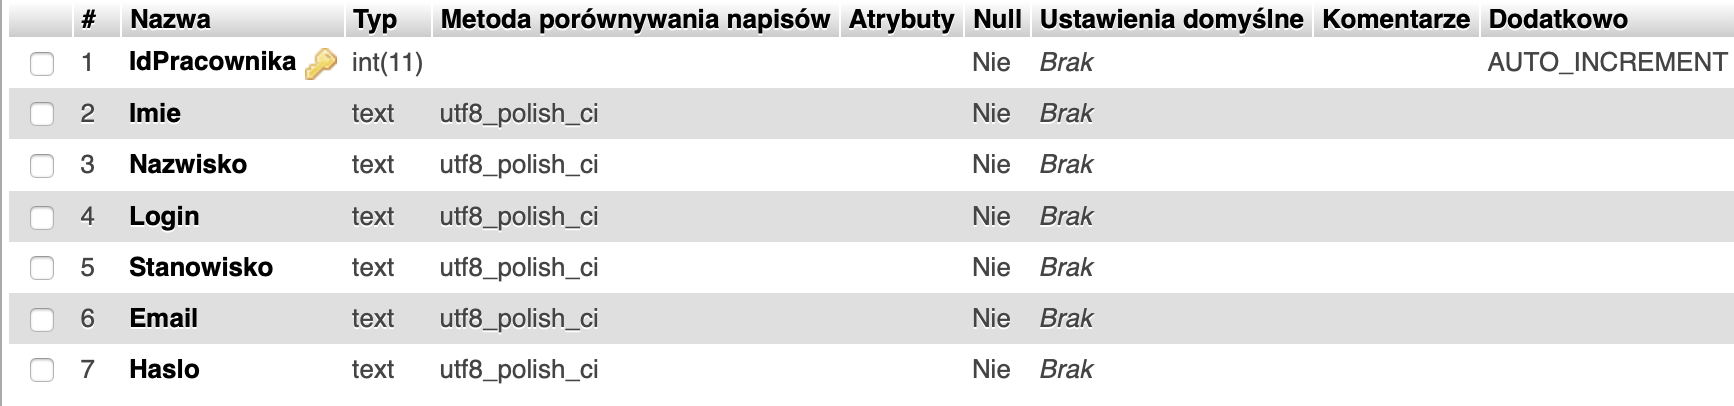
\includegraphics[width=0.75\textwidth]{pracownik}
	\label{tab:1}
\end{table}

\begin{table}[H]
	\centering
	\caption{Tabela klientów}
	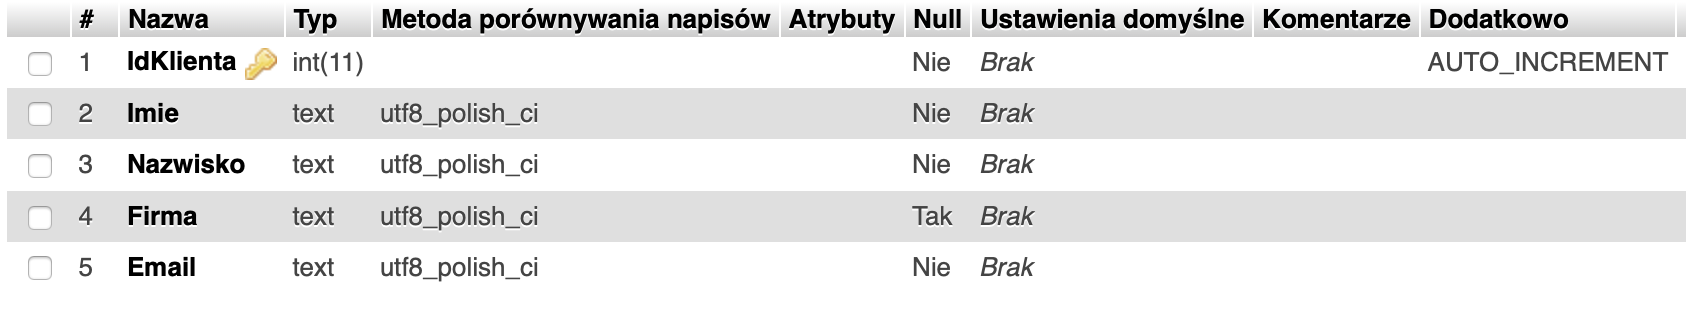
\includegraphics[width=0.75\textwidth]{klienci}
	\label{tab:2}
\end{table}

\begin{table}[H]
	\centering
	\caption{Tabela notatek}
	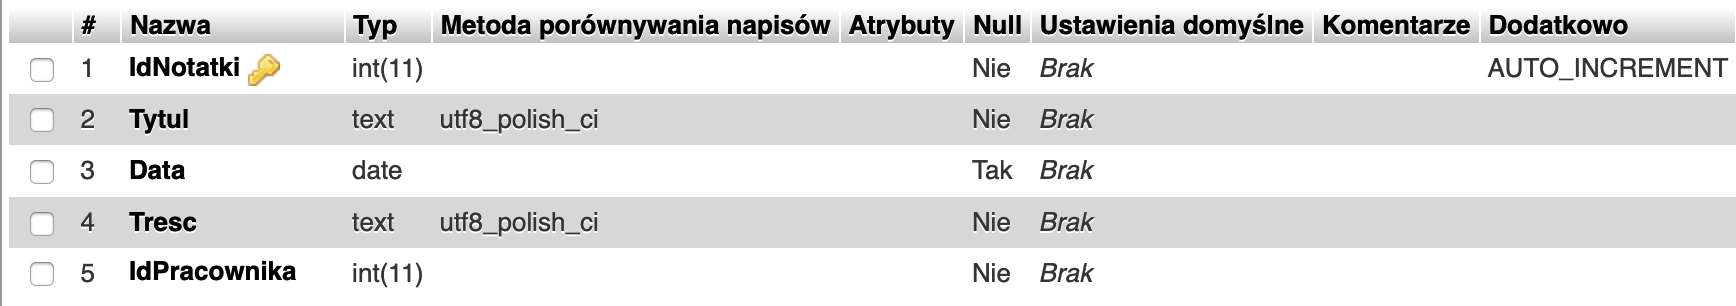
\includegraphics[width=0.75\textwidth]{tabelanotatki}
	\label{tab:3}
\end{table}

\begin{table}[H]
	\centering
	\caption{Tabela spotkań}
	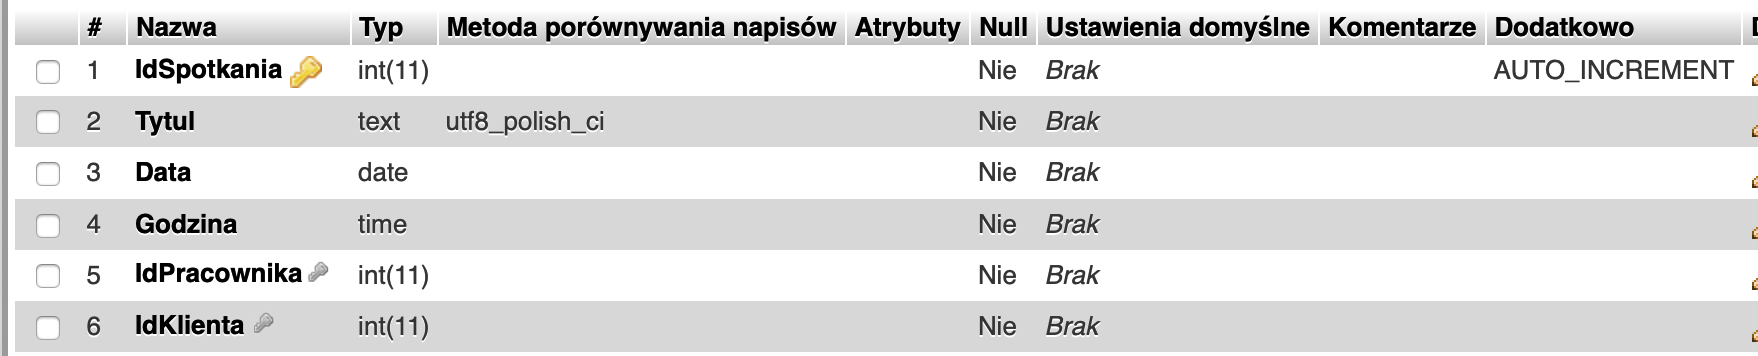
\includegraphics[width=0.75\textwidth]{spotkania}
	\label{tab:4}
\end{table}


\subsection*{Mechanizmy bezpieczeństwa}

W celu zachowania bezpieczeństwa ograniczono dostęp do danych przez mechanizm uprawnień. Uprawnienia poszczególnych użytkowników przedstawiono w Tabeli \ref{tab:5}.
\begin{table}[H]
	\centering
	
	\caption{Uprawnienia użytkowników do poszczególnych tabel w bazie danych}


	\begin{tabular}{c|c|c|c} 
	 & Użytkownik & Pracownik & Administrator \\ \hline
	Pracownicy & C & RU & CRUD \\ \hline
	Klienci & - & CRU & CRUD \\ \hline
	Notatki & - &CRUD & CRUD \\ \hline
	Spotkania & - & CRUD & CRUD 

	\end{tabular}
	\label{tab:5}
\end{table}


\section{Interfejs użytkownika}

Na stronie głównej interfejsu użytkownika znajduje się kafelkowe menu, w którym są następujące opcje do wyboru:
\begin{itemize}
	\item Dzień - wyświetlenie bieżącego dnia, razem z zaplanowanymi spotkaniami oraz notatkami. Za pomocą strzałek przy dacie można zmieniać dzień na poprzedni i kolejny. Po naciśnięciu na wybraną notatkę lub spotkanie można dokonać jej edycji.
	\item Miesiąc - wyświetla trwający miesiąc z podświetlonym dniem dzisiejszym, po prawej stronie są wypisane notatki na dany miesiąc. Dzięki strzałkom przy aktualnym miesiącu można zmieniać miesiąc w przód oraz w tył. Po naciśnięciu na notatkę można ją edytować. Przy wybraniu konkretnego dnia, aplikacja przeniesie pracownika do spotkań i notatek zaplanowanych na ten dzień (jak w zakładce 'Dzień').
	\item Rok - pokazuje bieżący rok, który można zmieniać analogicznie jak miesiąc i dzień, a także wybierać konkretny miesiąc, który przeniesie nas do zakładki 'Miesiąc' z wybranym miesiącem i rokiem. Po prawej stronie można zobaczyć notatki na wybrany rok i również wybrać jedną i dokonać edycji, a także dodać nową.
	\item Notatki - wyświetla spis wszystkich notatek, razem z tymi, które nie mają zaplanowanej konkretnej daty. Tu także jest możliwość dodania i edycji notatki.
	\item Zaloguj/Wyloguj - pierwsza opcja przenosi niezalogowanego użytkownika do panelu logowania i rejestracji, a druga pokazuje się jedynie użytkownikowi zalogowanemu. Po wybraniu tej opcji pracownik zostanie wylogowany.
	\item Dodaj spotkanie - wyświetla dwa formularze, jeden do dodania spotkania z wybranym klientem, a drugi do dodania klienta, żeby móc umówić z nim spotkanie.
	\item Dodaj notatkę - umożliwia dodanie nowej notatki
	\item W stopce aplikacji znajdują się dane osoby, która ją stworzyła oraz prawa autorskie
	
\end {itemize}




\newpage




Na Rysunku \ref{fig:3} przedstawiono stronę główną aplikacji dla niezalogowanego użytkownika, natomiast na Rysunku \ref{fig:4} wygląd strony głównej po zalogowaniu. \\


\begin{figure}[H]
	\centering
	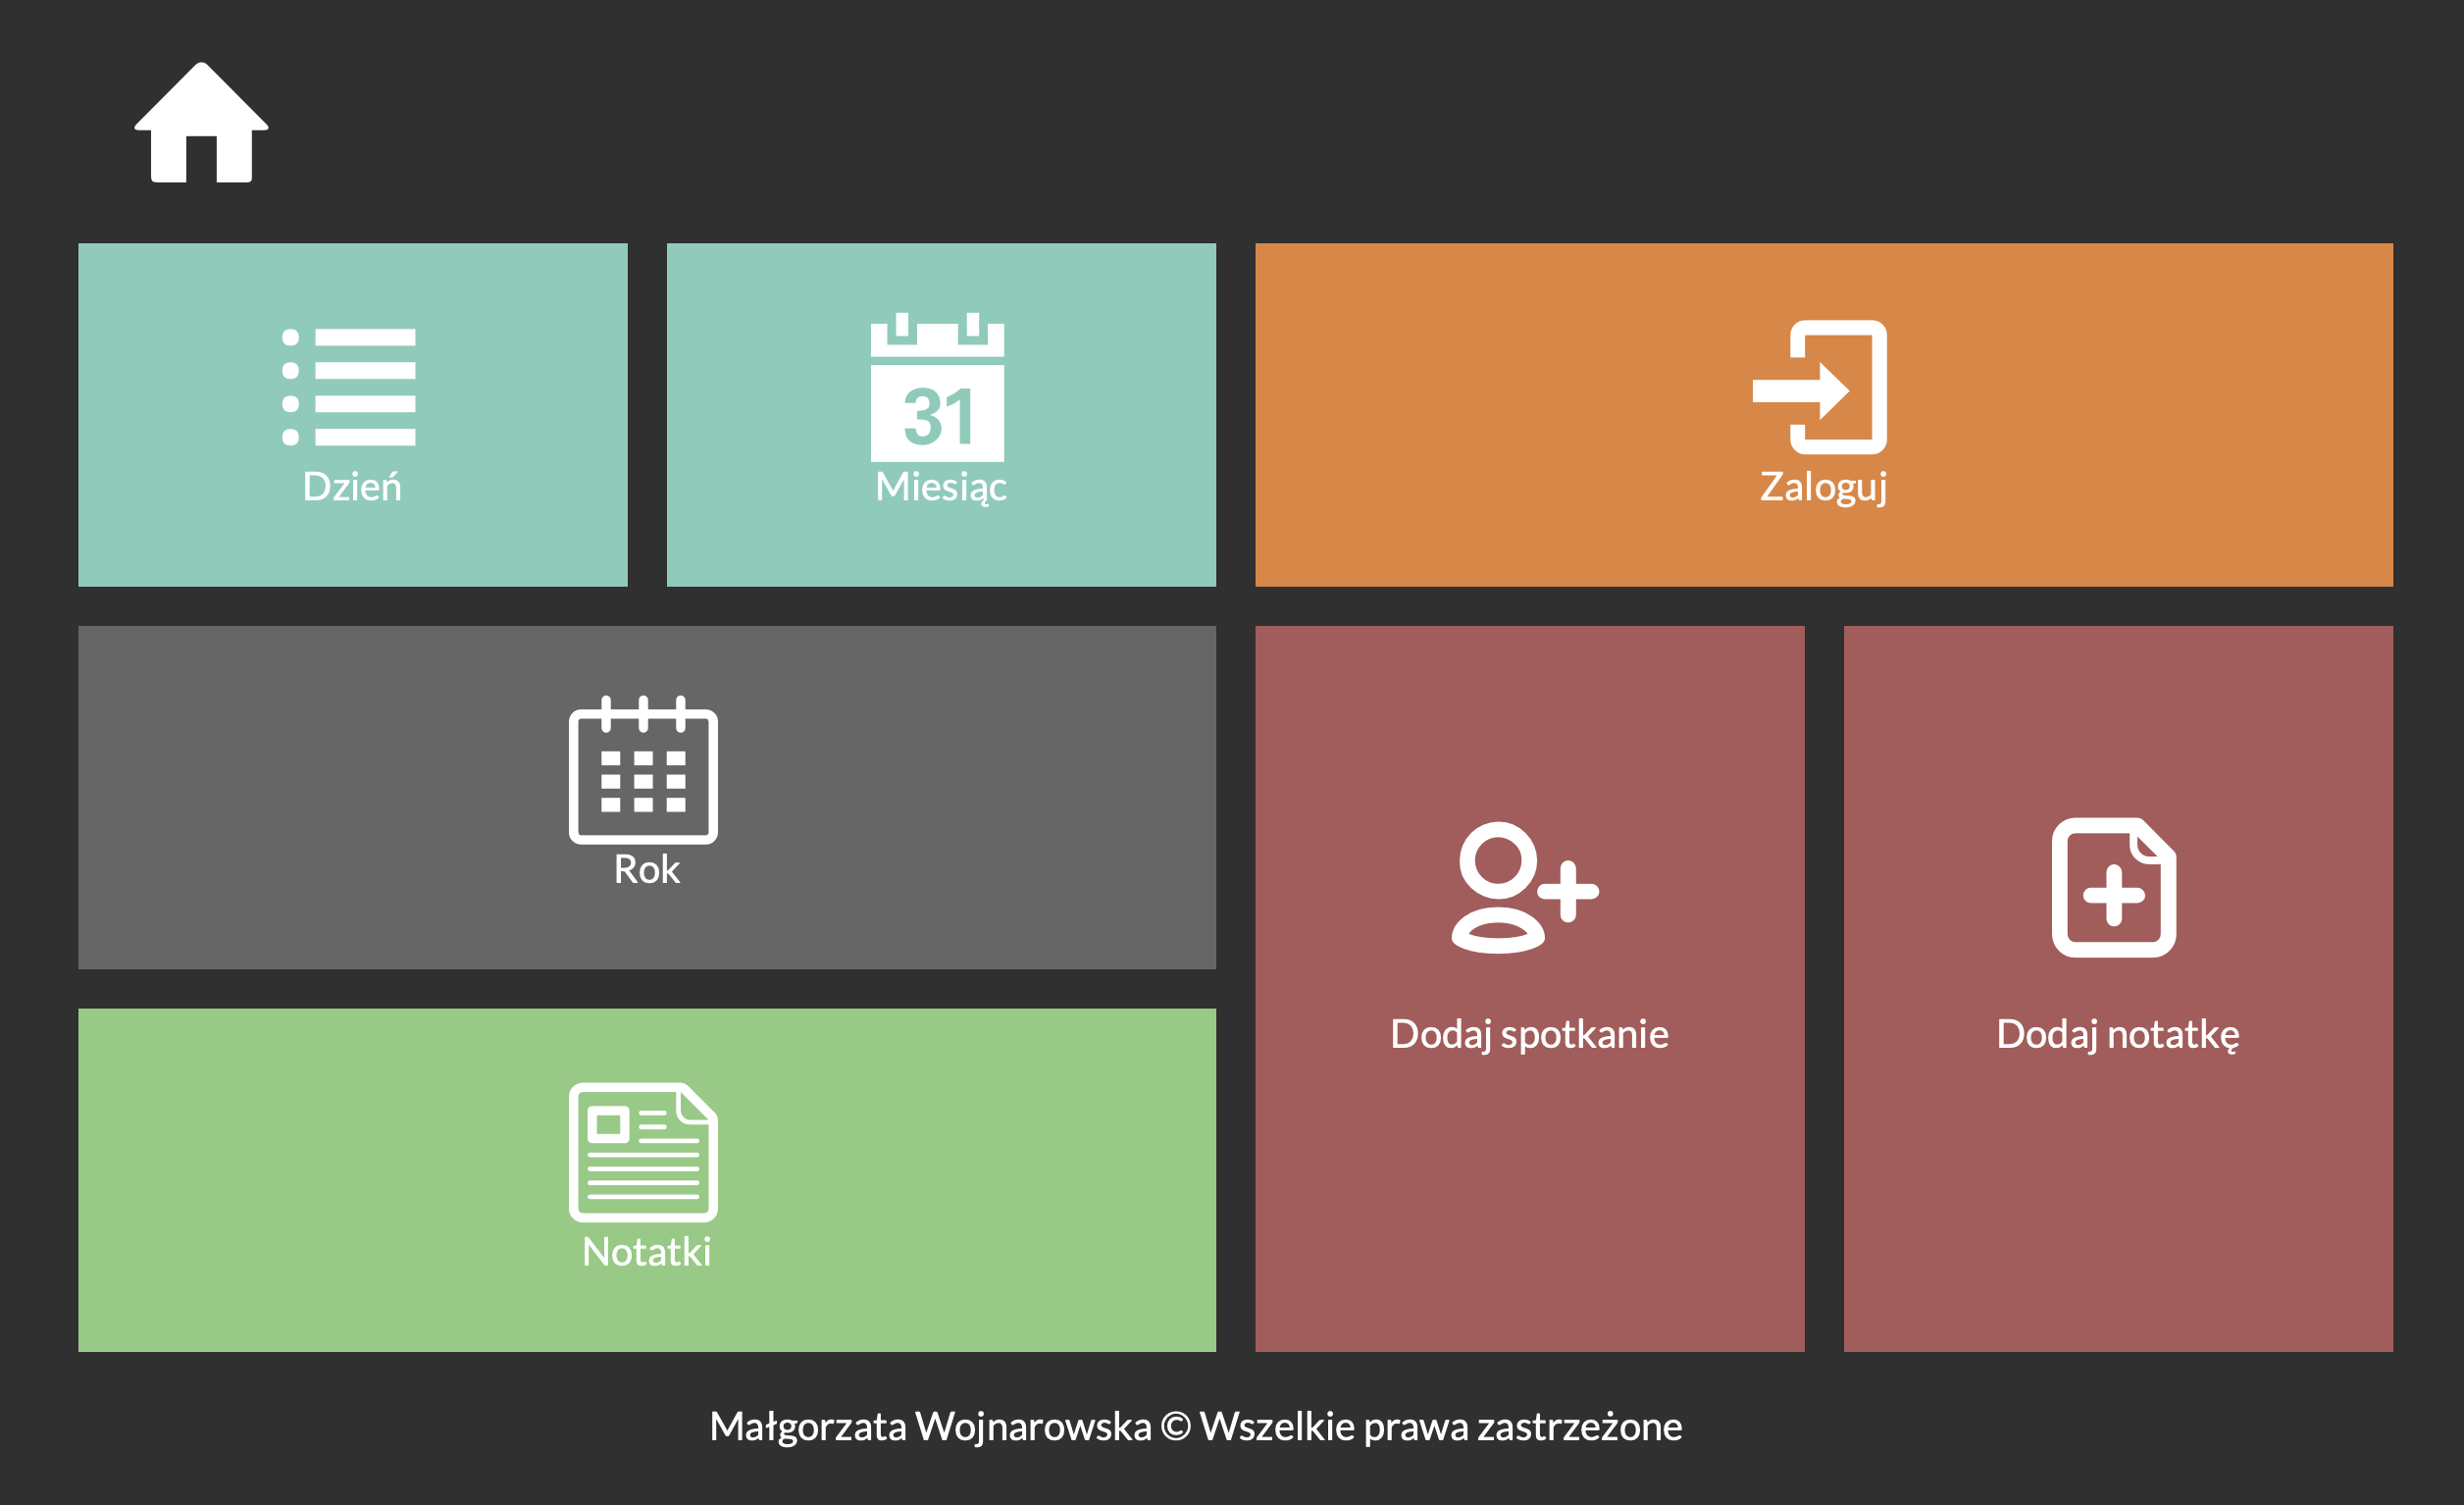
\includegraphics[width=0.75\textwidth]{niezalogowany}
	\caption{Strona główna dla niezalogowanego użytkownika}
	\label{fig:3}
\end{figure}




\begin{figure}[H]
	\centering
	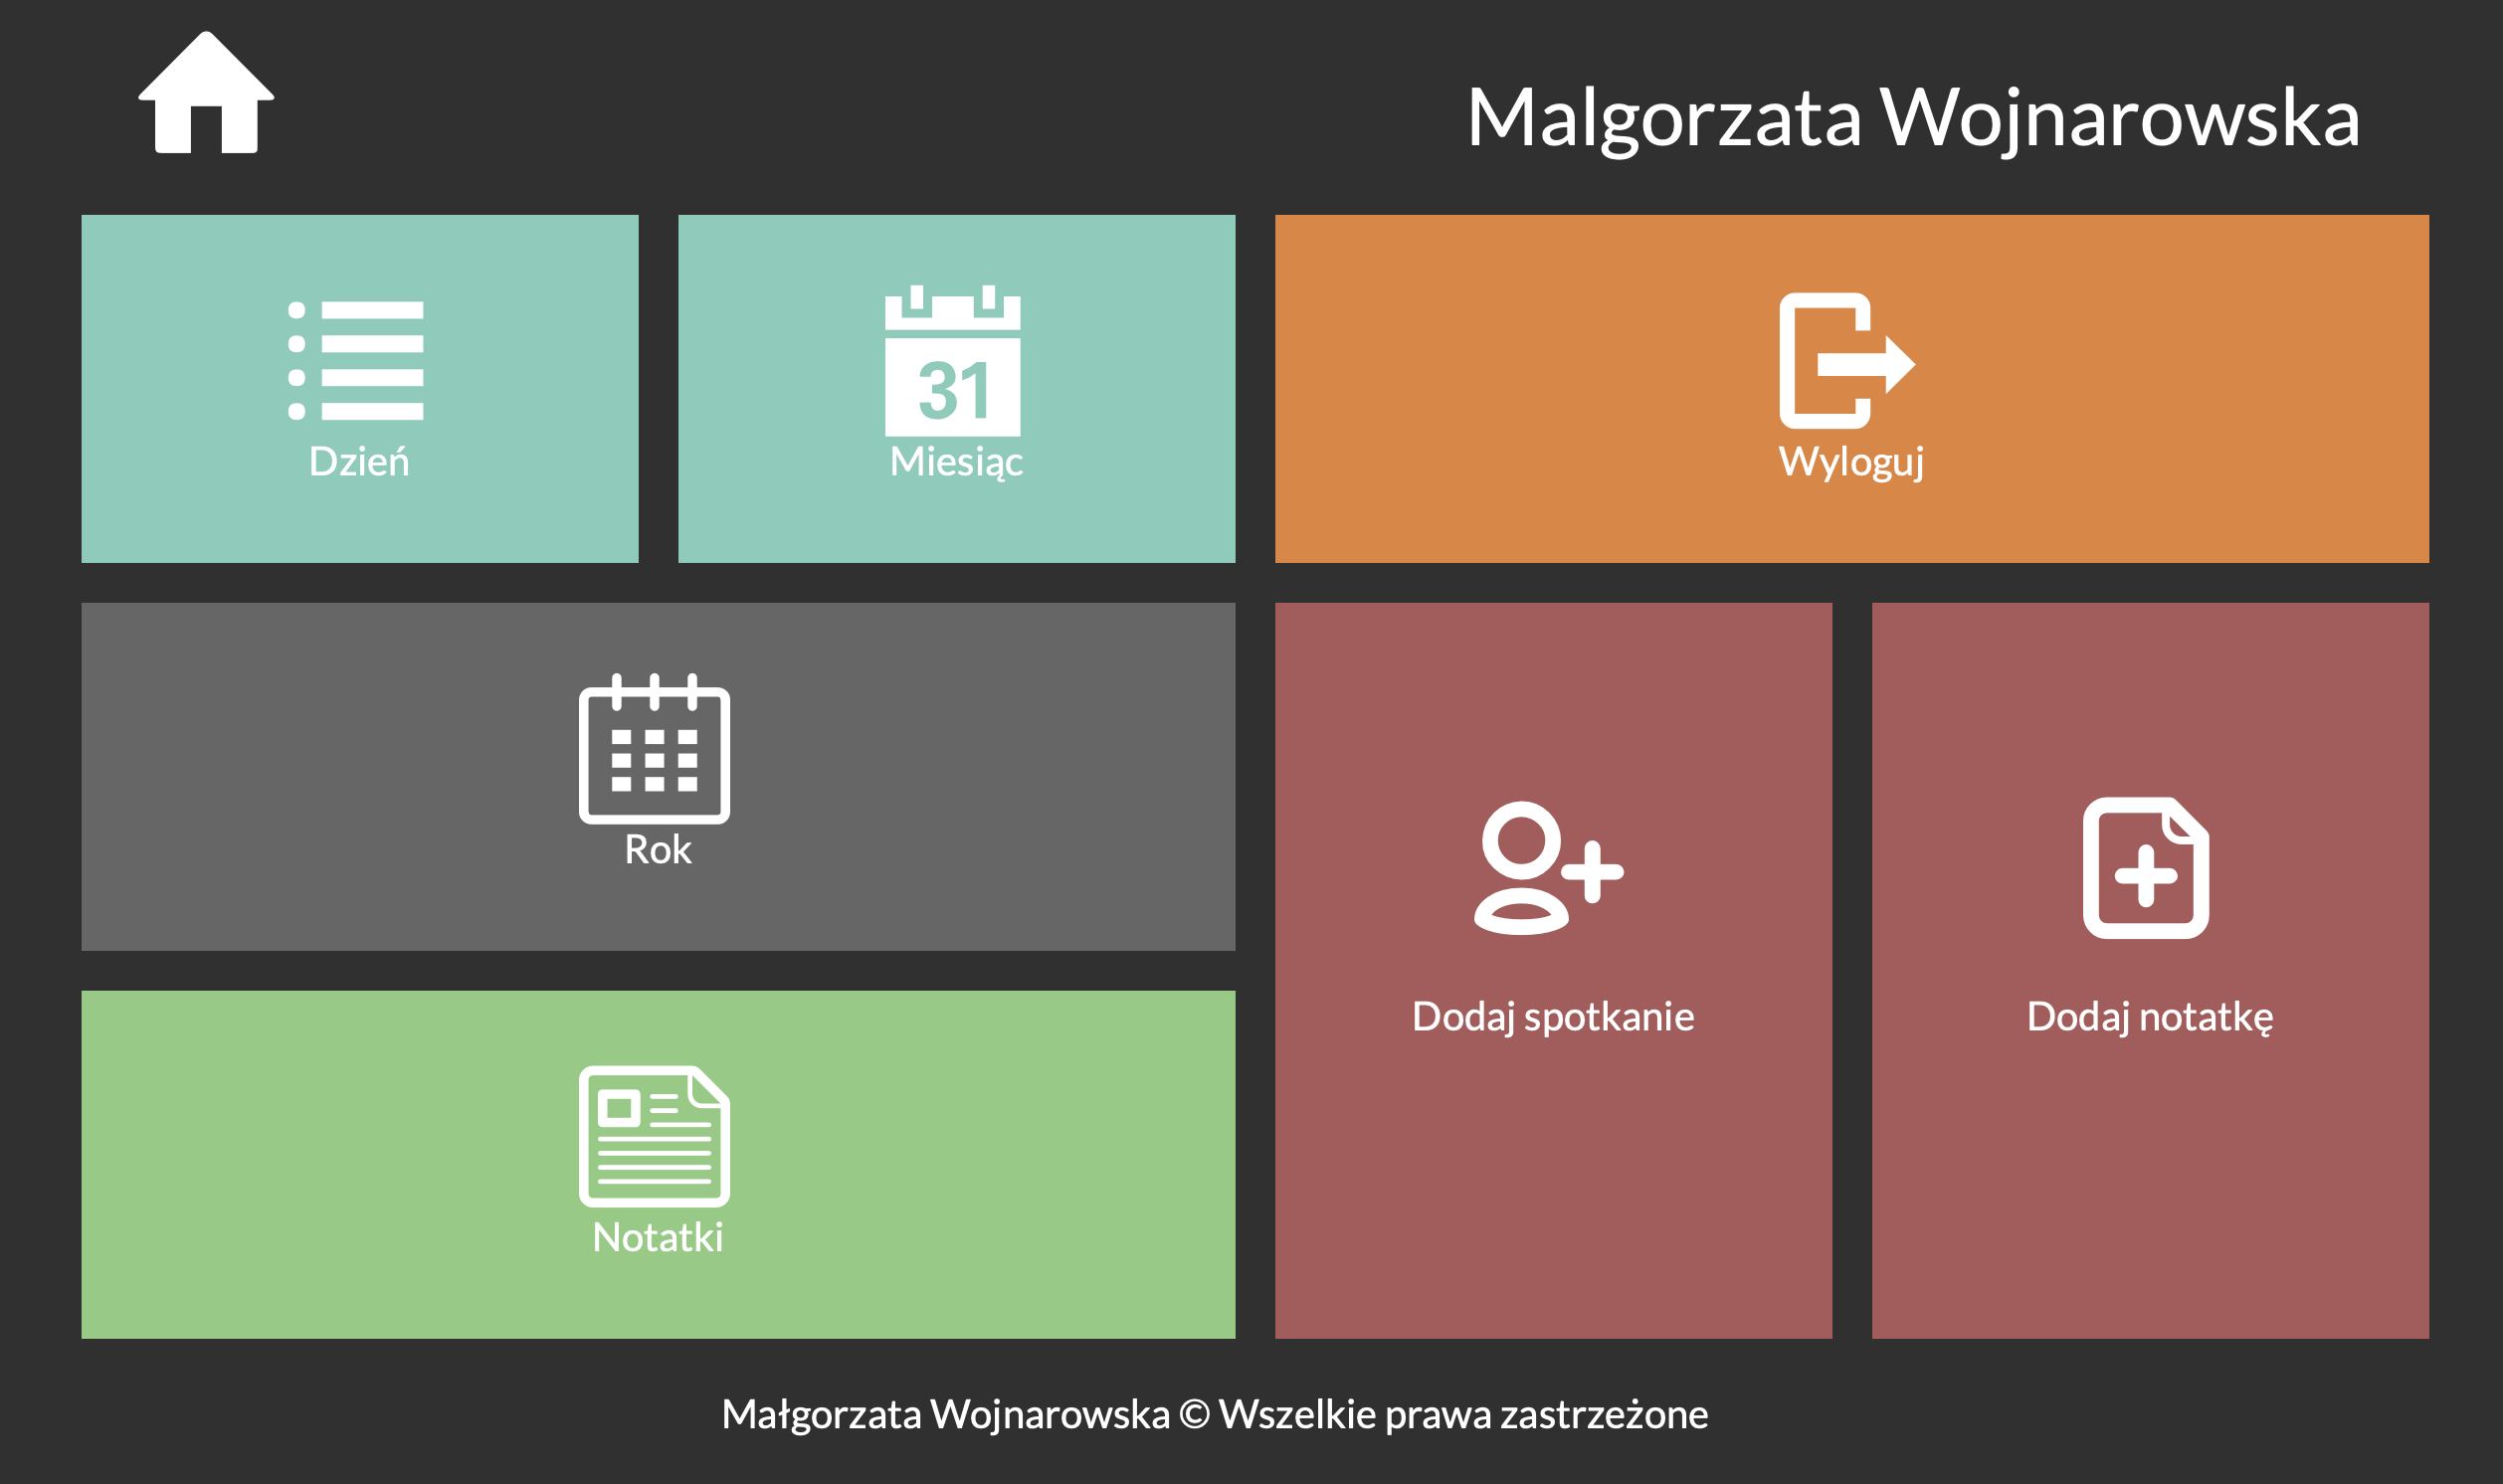
\includegraphics[width=0.75\textwidth]{strona_zalogowany}
	\caption{Strona główna dla zalogowanego pracownika}
	\label{fig:4}
\end{figure}



	\subsection*{Funkcja rejestracji nowego użytkownika}
	Przed zalogowaniem, kliknięcie dowolnego pola przeniesie użytkownika do panelu logowania. Tam nowy użytkownik może stworzyć konto po naciśnięciu przycisku "Zarejestruj się". W tym celu zostanie otworzona nowa podstrona z formularzem do rejestracji. Po wypełnieniu wszystkich pól i stworzeniu konta, użytkownik zostanie przeniesiony na stronę, która wyświetla komunikat o poprawnej rejestracji oraz przycisk do panelu logowania. Od teraz pracownik będzie mógł się zalogować przez wybrany login i hasło.

Panel logowania do aplikacji pokazany jest na Rysunku \ref{fig:5}.

\begin{figure}[H]
	\centering
	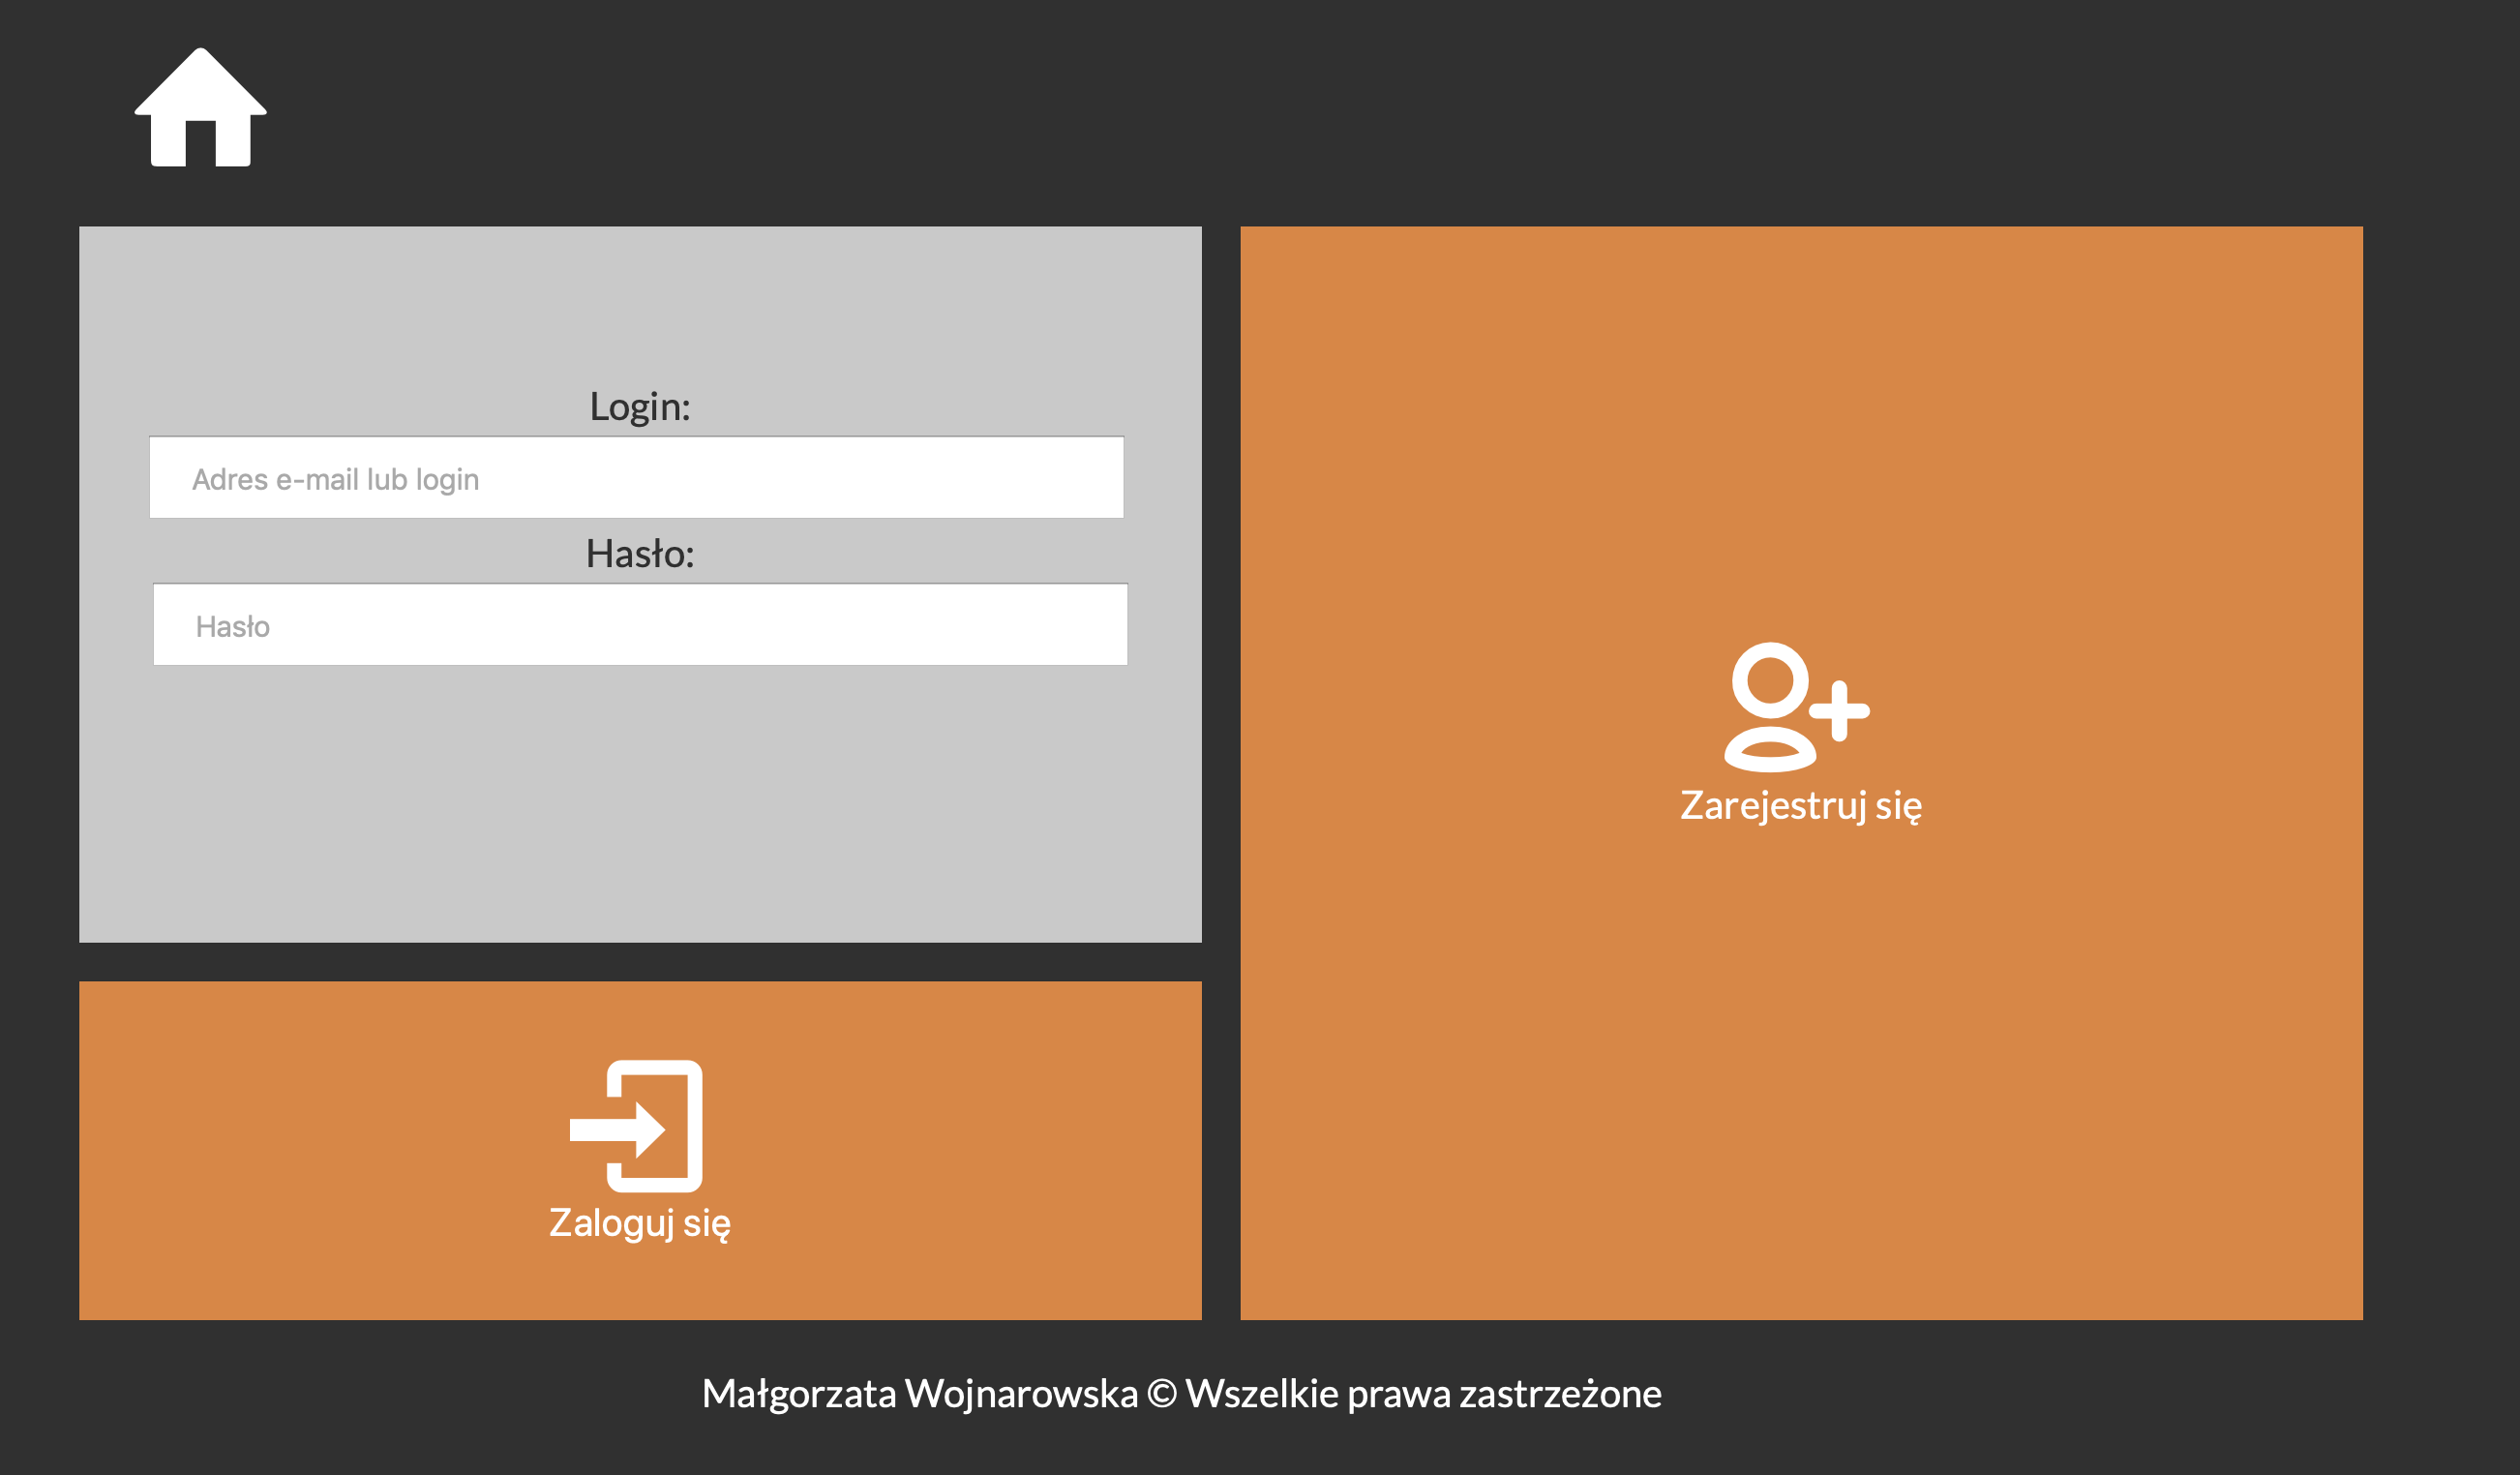
\includegraphics[width=0.75\textwidth]{logowanie}
	\caption{Panel logowania}
	\label{fig:5}
\end{figure}


	
	\subsection*{Funkcja dodawania i edycji klienta lub spotkania}
	Każdy zalogowany użytkownik ma możliwość dodania własnego spotkania oraz stworzenia klienta. Aby to zrobić należy wypełnić znajdujący się po prawej stronie formularz, który ukaże się po naciśnięciu przycisku "Dodaj spotkanie". Następnie za pomocą rozwijanej listy zalogowany pracownik ma możliwość zapisania spotkania z danym klientem za pomocą wyboru z listy rozwijanej. Aby dodać notatkę należy wypełnić analogiczny formularz po wyborze opcji "Dodaj notatkę". 

Na Rysunku \ref{fig:6} przedstawione jest dodawanie spotkania i klienta do bazy danych.

\begin{figure}[H]
	\centering
	
\includegraphics[width=0.75\textwidth]{dodaj_spotkanie_klient}
	\caption{Dodawanie spotkania lub klienta}
	\label{fig:6}
\end{figure}

	
	\subsection*{Funkcja przeglądania kalendarza, zapisanych spotkań oraz notatek}
	Pracownik może także przeglądać zapisane notatki oraz spotkania, segregując je za pomocą daty: konkretnego dnia, miesiąca oraz roku, a także wyświetlając wszystkie notatki bez względu na datę. Pracownik może za pomocą kliknięcia wybrać konkretny miesiąc oraz dzień. 

Dostępne funkcje przeglądania notatek oraz spotkań pokazane są na Rysunku \ref{fig:7}.
	
\begin{figure}[H]
	\centering
	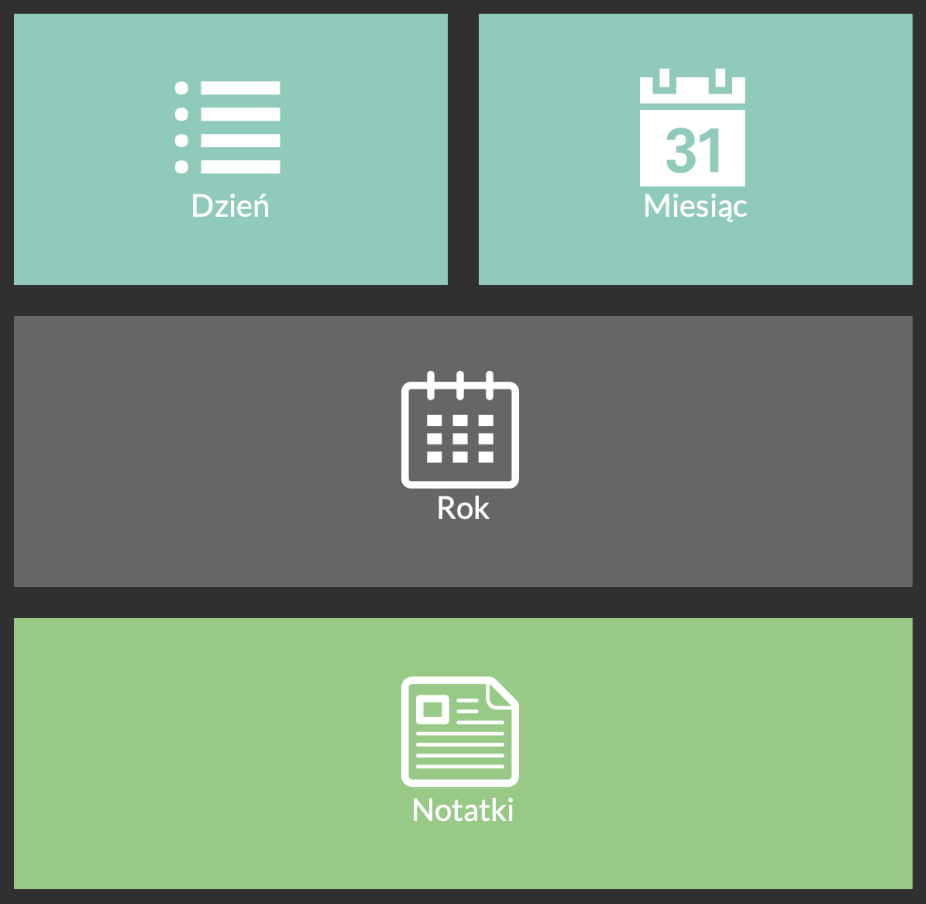
\includegraphics[width=0.5\textwidth]{przeglad}
	\caption{Przeglądanie kalendarza}
	\label{fig:7}
\end{figure}


	
	
	\subsection*{Funkcja dodawania oraz edycji notatki}
	Po zalogowaniu do systemu pracownik może także dowolnie dodawać oraz edytować spotkania i notatki. Aby to zrobić należy wybrać daną notatkę, która wyświetla się po prawej stronie dnia, miesiąca lub roku, a także po wyświetleniu listy wszystkich notatek.

Po wybraniu przycisku 'Dodaj notatkę' (Rysunek \ref{fig:8}) otwiera się formularz, który pozwala na stworzenie notatki.
	
\begin{figure}[H]
	\centering
	
\includegraphics[width=0.5\textwidth]{dodaj_notatke_edycja}
	\caption{Dodawanie notatki}
	\label{fig:8}
\end{figure}





\subsection*{Zabezpieczenia}

W aplikacji znajdują się pewne zabezpieczenia, które mają na celu zwiększenie bezpieczeństwa systemu. Zabezpieczenia są zarówno na poziomie bazy danych, jak i przy programowaniu aplikacji. Są to między innymi:

\begin{itemize}
	\item ograniczenie uprawnień dla poszczególnych użytkowników,
	\item przy rejestracji zabezpieczenie akceptacji regulaminu,
	\item przy wypełnianiu formularza adres e-mail musi mieć poprawną formę,
	\item podczas rejestracji login nie może zawierać znaków specjalnych,
	\item ograniczenie długości znaków podczas wypełniania formularzy,
	\item zabezpieczenie przed otwarciem podstron przez niezalogowanych użytkowników.
\end{itemize}

Podczas logowania wpisanie błędnego loginu lub hasła skutkuje błędem logowania, który przedstawiony jest na Rysunku \ref{fig:9}.

	\begin{figure}[H]
		\centering
		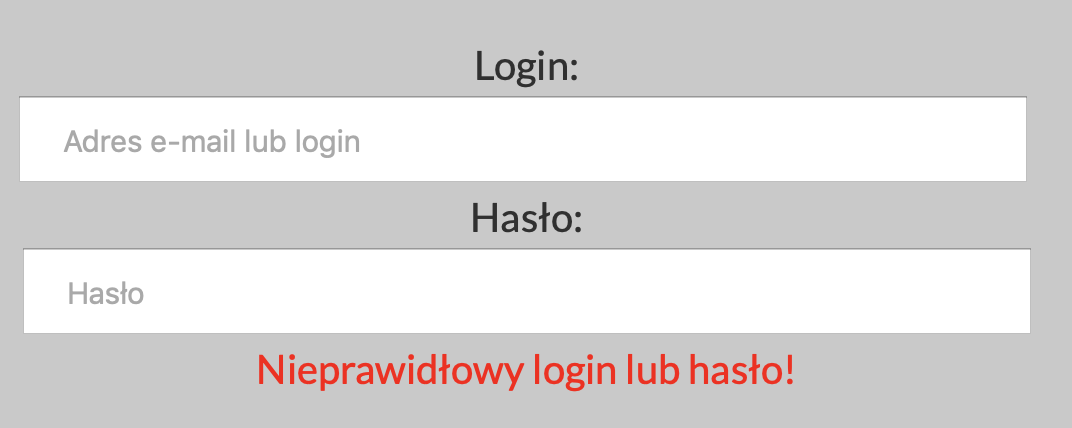
\includegraphics[width=0.75\textwidth]{blad_logowania}
		\caption{Błąd logowania}
		\label{fig:9}
	\end{figure}
	
Formularz rejestracji należy poprawnie wypełnić. Loginu, musi się składać jedynie z liter oraz cyfr, nie może zawierać polskich znaków. Login powinien mieć od 3 do 20 znaków. Jeśli ten warunek nie jest spełniony, to przy formularzu pojawi się błąd, który jest pokazany na Rysunku \ref{fig:10}. Ponieważ login musi być unikalny, błąd pojawi się także przy próbie wybrania loginu, który już znajduje się w bazie danych. Każdy z przypadków błędnego wpisania loginu skutkuje innym komunikatem o niepoprawności wypełnienia formularza.

	\begin{figure}[H]
		\centering
		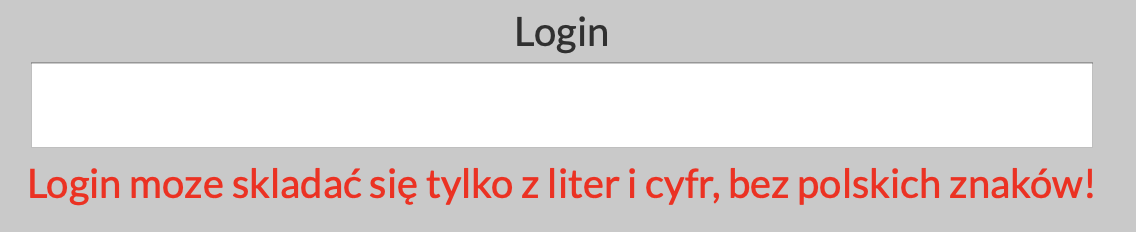
\includegraphics[width=0.75\textwidth]{rejestracja_login}
		\caption{Błąd loginu}
		\label{fig:10}
	\end{figure}
	
Podczas rejestracji sprawdzana jest także poprawność wpisanego e-maila. Ponieważ jeden e-mail może być przypisany do jednego konta, tutaj również sprawdzane jest, czy wybrany e-mail nie znajduje się już w bazie danych. W zależności od tego, który z tych warunków nie został spełniony, wyświetlany jest odpowiedni komunikat o błędzie. Jeśli użytkownik pomylił się w formie e-maila - na przykład nie wystąpił w nim znak '@' - zostanie wyświetlona wiadomość o błędzie z Rysunku \ref{fig:11}.
	
	\begin{figure}[H]
		\centering
		
\includegraphics[width=0.75\textwidth]{rejestracja_email}
		\caption{Błąd e-maila}
		\label{fig:11}
	\end{figure}
	
W formularzu rejestracji podane są dwa okna do wpisania hasła. Jedno z nich występuje po to, aby potwierdzić, że użytkownik nie pomylił się przy jego wpisywaniu. Dla bezpieczeństwa sprawdzamy, czy oba hasła podane przez użytkownika są takie same. Hasła muszą mieć od 3 do 20 znaków. Jeśli się nie zgadzają zostanie wyświetlony komunikat pokazany na Rysunku \ref{fig:12}.
	
	\begin{figure}[H]
		\centering
		
\includegraphics[width=0.75\textwidth]{rejestracja_haslo}
		\caption{Błąd hasła - podane hasła się różnią}
		\label{fig:12}
	\end{figure}

Aby uniknąć prawnych zażaleń użytkownik musi zaakceptować regulamin korzystania z aplikacji. Jest to także kontrola przed sztucznymi kontami, tworzonymi przez zaprogramowane algorytmy. Bez akceptacji konto pracownika nie zostanie stworzone, a w formularzu wyświetli się komunikat z Rysunku \ref{fig:13}.
	
	\begin{figure}[H]
		\centering
		
\includegraphics[width=0.75\textwidth]{rejestracja_regulamin}
		\caption{Błąd regulaminu - brak zaakceptowania}
		\label{fig:13}
	\end{figure}
	
	

\section{Diagram projektowy}

Korzystając z wymagań funkcjonalnych (patrz 3.2) został stworzony diagram prezentujący interakcję pomiędzy poszczególnymi grupami użytkowników, a aplikacją. Diagram ten znajduje się na Rysunku \ref{fig:14}.

\begin{figure}[H]
	\centering
	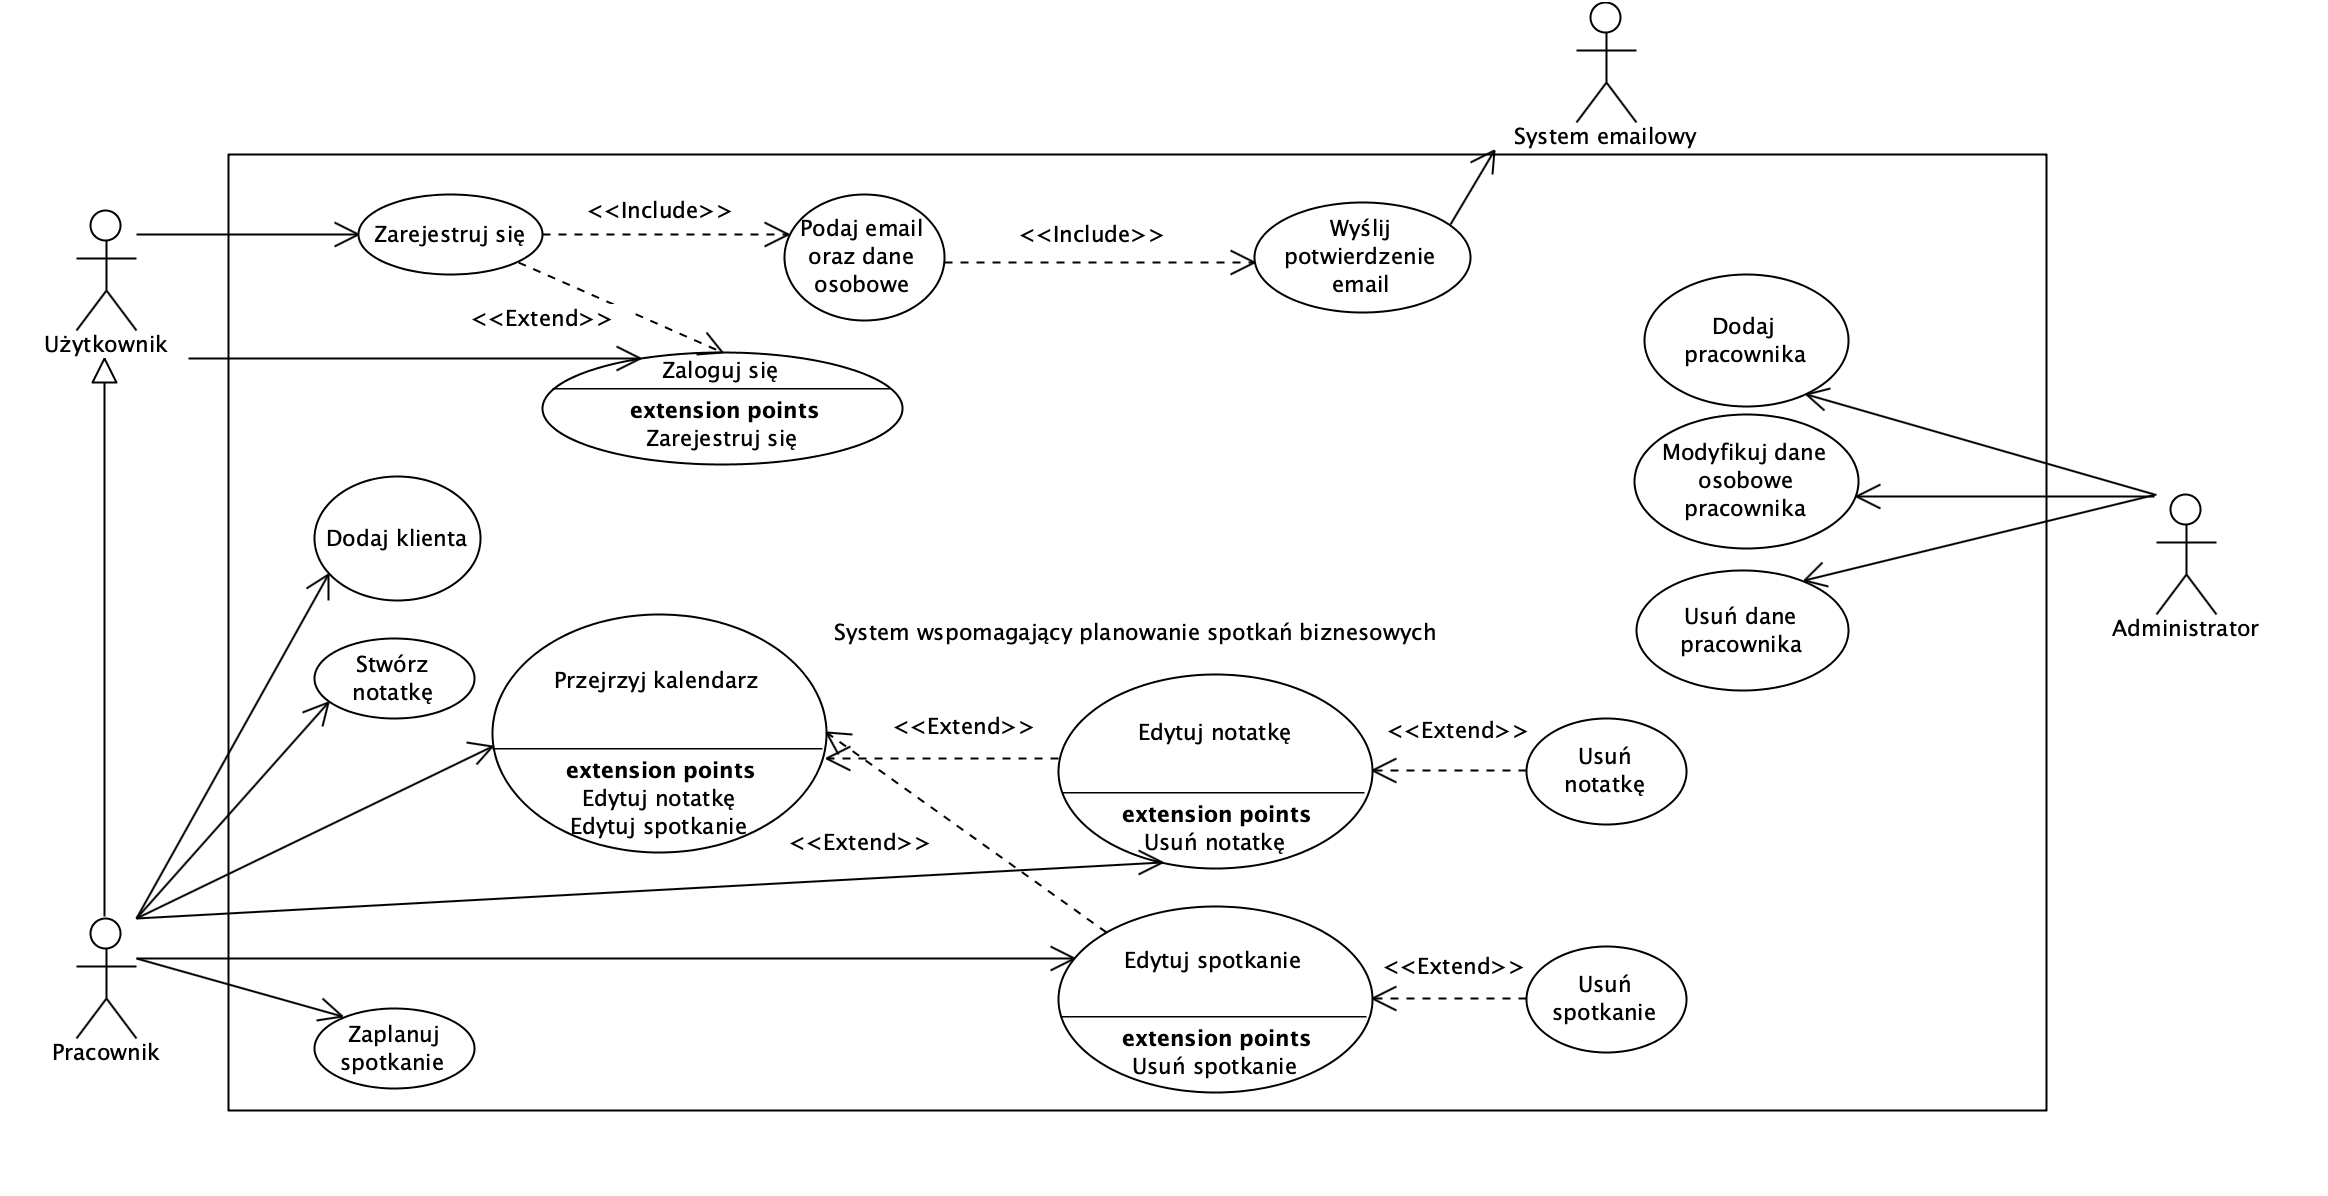
\includegraphics[width=1\textwidth]{diagram}
	\caption{Diagram przypadków użycia}
	\label{fig:14}
\end{figure}







\chapter{Implementacja systemu baz danych}
\section{Tworzenie tabel}

Aby zaprogramować użytkową aplikację, należy utworzyć relacyjną bazę danych, gdzie będą mogły być przechowywane informacje na temat klientów, pracowników, a także ich spotkań i osobistych notatek. Na początku tworzymy potrzebne nam tabele za pomocą języka SQL:
\begin{itemize}
\item tabela 'Spotkania', gdzie będą się znajdować informacje na temat spotkań pracowników, takie jak ich temat ('Tytul'), data oraz godzina spotkania, a także dane pracownika oraz klienta, z którym to spotkanie się odbędzie,
\item tabela 'Notatki' zawiera informacje na temat jej tytułu, treści, unikalnego indeksu 'IdPracownika', który stworzył tę notatkę, a także opcje daty, do której można, ale nie trzeba jej przypisać. Oznacza to, że notatka nie musi mieć daty,
\item tabela 'Klienci' przechowuje dane klientów. Znajdują się tam takie informacje jak imię i nazwisko klienta, firma, w której pracuje (może nie pracować w żadnej), a także jego e-mail do celów kontaktowych,
\item tabela 'Pracownicy', w której znajdują się ich dane, takie jak imię, nazwisko, stanowisko, e-mail a także indywidualny login i hasło, za pomocą których pracownik może zalogować się do systemu.
\end{itemize}
Wszystkie tabele mają zapisane kodowanie utf8, dzięki czemu w aplikacji można używać znaków polskich. Tworzenie poszczególnych tabel pokazane jest na Listingach \ref{lis:1}  - \ref{lis:4}.



\newpage




\begin{center}	
\begin{lstlisting}[caption={Stworzenie tabeli spotkań}, language=SQL, label={lis:1}]
CREATE TABLE `Spotkania` (
  `IdSpotkania` int(11) NOT NULL,
  `Tytul` text COLLATE utf8_polish_ci NOT NULL,
  `Data` date NOT NULL,
  `Godzina` time NOT NULL,
  `IdPracownika` int(11) NOT NULL,
  `IdKlienta` int(11) NOT NULL
) ENGINE=InnoDB DEFAULT CHARSET=utf8 COLLATE=utf8_polish_ci;
\end{lstlisting}
\end{center}
	
	
	
\begin{lstlisting}[caption={Stworzenie tabeli notatek}, language=SQL, label={lis:2}]
CREATE TABLE `Notatki` (
  `IdNotatki` int(11) NOT NULL,
  `Tytul` text COLLATE utf8_polish_ci NOT NULL,
  `Data` date DEFAULT NULL,
  `Tresc` text COLLATE utf8_polish_ci NOT NULL,
  `IdPracownika` int(11) NOT NULL
) ENGINE=InnoDB DEFAULT CHARSET=utf8 COLLATE=utf8_polish_ci;
\end{lstlisting}
	
\begin{lstlisting}[caption={Stworzenie tabeli klientów}, language=SQL, label={lis:3}]
CREATE TABLE `Klienci` (
  `IdKlienta` int(11) NOT NULL,
  `Imie` text COLLATE utf8_polish_ci NOT NULL,
  `Nazwisko` text COLLATE utf8_polish_ci NOT NULL,
  `Firma` text COLLATE utf8_polish_ci,
  `Email` text COLLATE utf8_polish_ci NOT NULL
) ENGINE=InnoDB DEFAULT CHARSET=utf8 COLLATE=utf8_polish_ci;
\end{lstlisting}	
	
\begin{lstlisting}[caption={Stworzenie tabeli pracowników}, language=SQL, label={lis:4}]
CREATE TABLE `Pracownicy` (
  `IdPracownika` int(11) NOT NULL,
  `Imie` text COLLATE utf8_polish_ci NOT NULL,
  `Nazwisko` text COLLATE utf8_polish_ci NOT NULL,
  `Login` text COLLATE utf8_polish_ci NOT NULL,
  `Stanowisko` text COLLATE utf8_polish_ci NOT NULL,
  `Email` text COLLATE utf8_polish_ci NOT NULL,
  `Haslo` text COLLATE utf8_polish_ci NOT NULL
) ENGINE=InnoDB DEFAULT CHARSET=utf8 COLLATE=utf8_polish_ci;
\end{lstlisting}
	
	
	

	
	
	
\section{Definiowanie indeksów oraz ograniczeń}

Aby relacyjna baza danych była funkcjonalna, tworzymy relacje pomiędzy poszczególnymi tabelami. W tabeli 'Notatki' dodajemy klucz obcy 'IdPracownika', który wiąże tę tabelę z tabelą 'Pracownicy'. Dzięki temu, każdy pracownik ma swoje notatki i nie ma dostępu do notatek współpracowników.

Analogicznie dodajemy klucz obcy 'IdPracownika' do tabeli 'Spotkania'. Tam dodajemy także klucz obcy 'IdKlienta', żeby łatwo rozpoznać z kim pracownik umówił dane spotkanie.

Tworzenie indeksów dla tabel 'Klienci', 'Notatki', 'Pracownicy' oraz 'Spotkania' pokazane jest kolejno na Listingu \ref{lis:5}, natomiast ograniczenia tabel 'Notatki' i 'Spotkania' znajdują się na Listingu \ref{lis:6}.
	
	
\begin{lstlisting}[caption={Tworzenie indeksów dla tabel}, language=SQL, label={lis:5}]
--
-- Indeksy dla tabeli `Klienci`
--
ALTER TABLE `Klienci`
  ADD PRIMARY KEY (`IdKlienta`);

--
-- Indeksy dla tabeli `Notatki`
--
ALTER TABLE `Notatki`
  ADD PRIMARY KEY (`IdNotatki`),
  ADD KEY `napisana przez` (`IdPracownika`);

--
-- Indeksy dla tabeli `Pracownicy`
--
ALTER TABLE `Pracownicy`
  ADD PRIMARY KEY (`IdPracownika`);

--
-- Indeksy dla tabeli `Spotkania`
--
ALTER TABLE `Spotkania`
  ADD PRIMARY KEY (`IdSpotkania`),
  ADD KEY `z` (`IdKlienta`),
  ADD KEY `spotyka sie` (`IdPracownika`) USING BTREE;

\end{lstlisting}
	

	
\begin{lstlisting}[caption={Ograniczenia tabel}, language=SQL, label={lis:6}]
--
-- Ograniczenia dla tabeli `Notatki`
--
ALTER TABLE `Notatki`
  ADD CONSTRAINT `napisana przez` FOREIGN KEY (`IdPracownika`) REFERENCES `inzynierka`.`Pracownicy` (`IdPracownika`) ON DELETE CASCADE ON UPDATE CASCADE;

--
-- Ograniczenia dla tabeli `Spotkania`
--
ALTER TABLE `Spotkania`
  ADD CONSTRAINT `spotyka sie` FOREIGN KEY (`IdPracownika`) REFERENCES `inzynierka`.`Pracownicy` (`IdPracownika`) ON DELETE CASCADE ON UPDATE CASCADE,
  ADD CONSTRAINT `z` FOREIGN KEY (`IdKlienta`) REFERENCES `inzynierka`.`Klienci` (`IdKlienta`) ON DELETE CASCADE ON UPDATE CASCADE;
COMMIT;
\end{lstlisting}
	
	
Automatyczne numerowanie indeksów (auto\_increment) sprawia, że użytkownik bazy danych nie musi się martwić o numerację rekordów. Jest to atrybut klucza głównego, który musi być unikalny dla każdego rekordu w tabeli. Implementacja kolejno dla tabel 'Klienci', 'Notatki', 'Pracownicy' oraz 'Spotkania' jest przedstawiona na Listingu \ref{lis:7}.
	
	
\begin{lstlisting}[caption={Automatyczne numerowanie indeksów}, language=SQL, label={lis:7}]
--
-- AUTO_INCREMENT dla tabeli `Klienci`
--
ALTER TABLE `Klienci`
  MODIFY `IdKlienta` int(11) NOT NULL AUTO_INCREMENT, AUTO_INCREMENT=6;

--
-- AUTO_INCREMENT dla tabeli `Notatki`
--
ALTER TABLE `Notatki`
  MODIFY `IdNotatki` int(11) NOT NULL AUTO_INCREMENT, AUTO_INCREMENT=17;

--
-- AUTO_INCREMENT dla tabeli `Pracownicy`
--
ALTER TABLE `Pracownicy`
  MODIFY `IdPracownika` int(11) NOT NULL AUTO_INCREMENT, AUTO_INCREMENT=5;

--
-- AUTO_INCREMENT dla tabeli `Spotkania`
--
ALTER TABLE `Spotkania`
  MODIFY `IdSpotkania` int(11) NOT NULL AUTO_INCREMENT, AUTO_INCREMENT=23;
\end{lstlisting}
	

\section{Nadawanie uprawnień użytkownikom}

Na podstawie Tabeli 3.5 nadano uprawnienia użytkownikom. Przykłady nadawanych uprawnień znajdują się na Listingach \ref{lis:8} oraz \ref{lis:9}.


\begin{lstlisting}[caption={Nadanie uprawnień w całej bazie danych dla administratora}, language=SQL, label={lis:8}]
GRANT ALL PRIVILEGES ON `inzynierka`.* TO `admin`@`localhost`;
\end{lstlisting}



\begin{lstlisting}[caption={Przykładowe uprawnienia do tabel Notatki i Klienci dla pracownika}, language=SQL, label={lis:9}]
GRANT ALL PRIVILEGES ON `Notatki` TO `pracownik`@`localhost`;
GRANT SELECT, INSERT, UPDATE PRIVILEGES ON `Klienci` TO `pracownik`@`localhost`;
\end{lstlisting}

	

\section{Testowanie bazy danych}

W ramach testów dodajemy przykładowe dane klienta za pomocą zapytania SQL (Listing \ref{lis:10}), a następnie wyświetlamy tabelę 'Klienci' (Listing \ref{lis:11}), aby sprawdzić, czy klient został dodany poprawnie. Tabela 'Klienci' po wykonaniu dwóch powyższych zapytań wyświetla się jak na Tabeli \ref{tab:6}.



\newpage



\begin{lstlisting}[caption={Przykład dodawania klienta}, language=SQL, label={lis:10}]
INSERT INTO `Klienci` (`IdKlienta`, `Imie`, `Nazwisko`, `Firma`, `Email`) VALUES (NULL, 'Katarzyna', 'Nowak', 'Atos', 'katarzyna.nowak@atos.com');
\end{lstlisting}


\begin{lstlisting}[caption={Wyświetlanie tabeli 'Klienci'}, language=SQL, label={lis:11}]
SELECT * FROM `Klienci`;
\end{lstlisting}


	\begin{table}[H]
		\centering
		\caption{Wynik zapytań na tabeli 'Klienci'}
		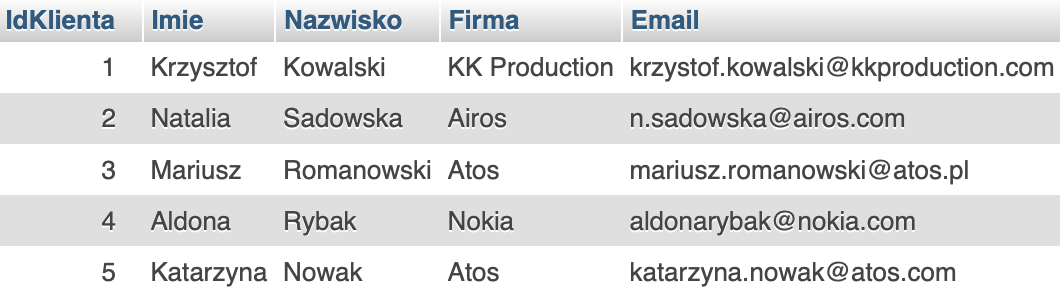
\includegraphics[width=0.75\textwidth]{baza_select_tabela}
		\label{tab:6}
	\end{table}
	
Kolejnym testem jest wyświetlenie tabeli 'Notatki' dla pracownika o określonym indeksie. Wynik zapytania z Listingu \ref{lis:12} znajduje się w Tabeli \ref{tab:7}.

\begin{lstlisting}[caption={Wyświetlanie tabeli 'Notatki' dla pracownika o indeksie 4}, language=SQL, label={lis:12}]
SELECT * FROM `Notatki` WHERE `IdPracownika`='4';
\end{lstlisting}	
	
	\begin{table}[H]
		\centering
		\caption{Tabela 'Notatki' dla pracownika o IdPracownika='4'}
		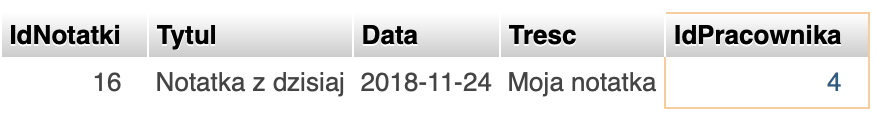
\includegraphics[width=0.75\textwidth]{baza_select_id_tabela}
		\label{tab:7}
	\end{table}
	
Zapytanie SELECT z Listingu \ref{lis:13} wyświetla wybrane kolumny z tabeli 'Pracownicy'. W tym przypadku są to kolumny indeksu pracownika, jego login oraz hasło w zaszyfrowanej postaci. Wynik zapytania przestawia Tabela \ref{tab:8}.
	
	
\begin{lstlisting}[caption={Wyświetlanie wybranych kolumn z tabeli 'Pracownicy'}, language=SQL, label={lis:13}]
SELECT `IdPracownika`, `Login`, `Haslo` FROM `Pracownicy`;
\end{lstlisting}

		
	\begin{table}[H]
		\centering
		\caption{Wynik zapytania 'SELECT' na tablicy 'Pracownicy'}
		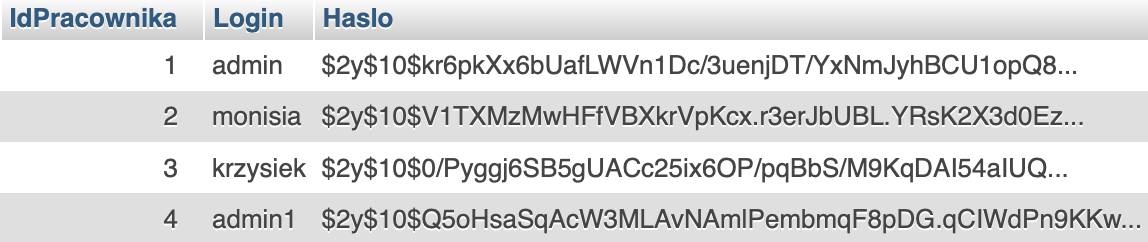
\includegraphics[width=0.75\textwidth]{baza_select_wybrane_tabela}
		\label{tab:8}
	\end{table}
	
Dodawanie oraz wyświetlanie rekordów działa prawidłowo. Dane są poprawnie odczytywane oraz kodowane. Hasło pracownika jest zaszyfrowane ze względów bezpieczeństwa.


\chapter{Implementowanie i testowanie aplikacji}

\section{Instalacja i konfigurowanie systemu}
Do uruchomienia aplikacji należy pobrać oraz uruchomić serwer lokalny XAMPP, a następnie odpalić moduł Apache oraz MySQL. Następnie otworzyć przeglądarkę i wejść na stronę localhost/phpmyadmin, gdzie należy importować bazę danych. Wszystkie pliki aplikacji powinny znajdować się w folderze /htdocs. Po wykonaniu tych akcji należy wpisać w okno przeglądarki adres localhost/aplikacja.


\section{Instrukcja użytkowania aplikacji}

Aplikacja została stworzona tak, aby była prosta w obsłudze. Jej kafelkowy wygląd sprawia, że obsługa jest intuicyjna dla każdego użytkownika. Instrukcje przykładowych funkcji znajdują się poniżej.

\subsection*{Instrukcja rejestracji pracownika}

Rejestrację może wykonać każdy użytkownik, który odwiedza stronę. Aby stworzyć nowe konto, należy:

	\begin{enumerate*}
		\item wejść w panel logowania,
		\item wypełnić formularz ze swoimi danymi, takimi jak imię, nazwisko, a także login i~hasło,
		\item zaakceptować regulamin,
		\item potwierdzić chęć rejestracji za pomocą wybrania przycisku 'Zarejestruj się'.
	\end{enumerate*}
	
Po wykonaniu tej instrukcji użytkownikowi zostanie wyświetlona informacja o poprawnie dokonanej rejestracji. Następnie będzie mógł się zalogować na swoje konto za pomocą wybranego loginu oraz hasła.

\subsection*{Instrukcja dodania klienta}

Instrukcja przeznaczona jest dla zalogowanego pracownika. Aby dodać klienta, należy:

	\begin{enumerate*}
		\item zalogować się za pomocą loginu (lub e-maila) oraz hasła,
		\item wejść w zakładkę 'Dodaj spotkanie',
		\item wypełnić formularz z danymi klienta,
		\item potwierdzić dane klienta wybierając opcję 'Dodaj klienta'.
	\end{enumerate*}
	
Po wykonaniu tych czynności klient zostanie dodany do bazy danych. Pracownikowi wyświetli się komunikat o poprawnie dodanym kliencie. Następnie pracownik będzie mógł wybrać opcję 'Dodaj spotkanie' i umówić spotkanie z tym klientem.

\subsection*{Instrukcja edycji notatki}

Edycja notatki jest dostępna jedynie dla zalogowanego pracownika. Aby mieć dostęp do tej funkcji, pracownik musi wcześniej mieć stworzoną chociaż jedną notatkę. Aby edytować istniejącą notatkę, należy:

	\begin{enumerate*}
		\item zalogować się na swoje konto pracownika,
		\item wejść w jedną z wymienionych zakładek: 'Dzień', 'Miesiąc', 'Rok' lub 'Notatki',
		\item nacisnąć na tytuł wybranej notatki,
		\item wybrać opcję 'Edytuj', która się pojawi po wybraniu notatki,
		\item edytować wybrane dane notatki,
		\item potwierdzić zmiany za pomocą przycisku 'Zapisz'.
	\end{enumerate*}
	
Po edycji notatki zostanie wyświetlona podstrona z komunikatem o poprawnej edycji. Pracownik może edytować notatki dowolną liczbę razy.
	
\subsection*{Instrukcja usuwania spotkania}

Aby usunąć spotkanie trzeba być zalogowanym pracownikem, a także mieć stworzone przynajmniej jedno spotkanie. Aby je usunąć, należy:

	\begin{enumerate*}
		\item zalogować się z panelu logowania,
		\item wejść w zakładkę 'Rok', 'Miesiąc' lub 'Dzień',
		\item przejść do wybranej daty,
		\item wybrać odpowiednie spotkanie naciskając tytuł spotkania,
		\item wybrać przycisk 'Edytuj', który pojawi się zamiast opcji 'Dodaj spotkanie',
		\item nacisnąć przycisk 'Usuń', nie wypełniając formularza, który się pojawi.
	\end{enumerate*}

Po wykonaniu tych czynności zostanie wyświetlony komunikat o poprawnym usunięciu spotkania. Usuniętego spotkania nie da się przywrócić.

\section{Użycie funkcji systemu}

\subsection{Zabezpieczenie stron dla niezalogowanych użytkowników}

Niezalogowany użytkownik nie ma dostępu do żadnych funkcji aplikacji, poza stroną główną, rejestracji i logowania. Przy próbie dostania się na dowolną inną podstronę, automatycznie zostaje przekierowany na stronę logowania.



\subsection{Tworzenie spotkań i klientów}

Na stronie głównej, a także na podstronach 'Dzień', 'Miesiąc' i 'Rok' znajduje się przycisk prowadzący do zakładki, która umożliwia tworzenie spotkań z klientami. Wygląd podstrony pokazany jest na Rysunku \ref{fig:15}. Jeśli klient nie istnieje jeszcze w bazie danych, można go dodać po prawej stronie zakładki. Po dodaniu go do bazy danych, pojawi się on w~liście rozwijanej przy wyborze klienta do umówienia spotkania (Rysunek \ref{fig:16}).

	\begin{figure}[H]
		\centering
		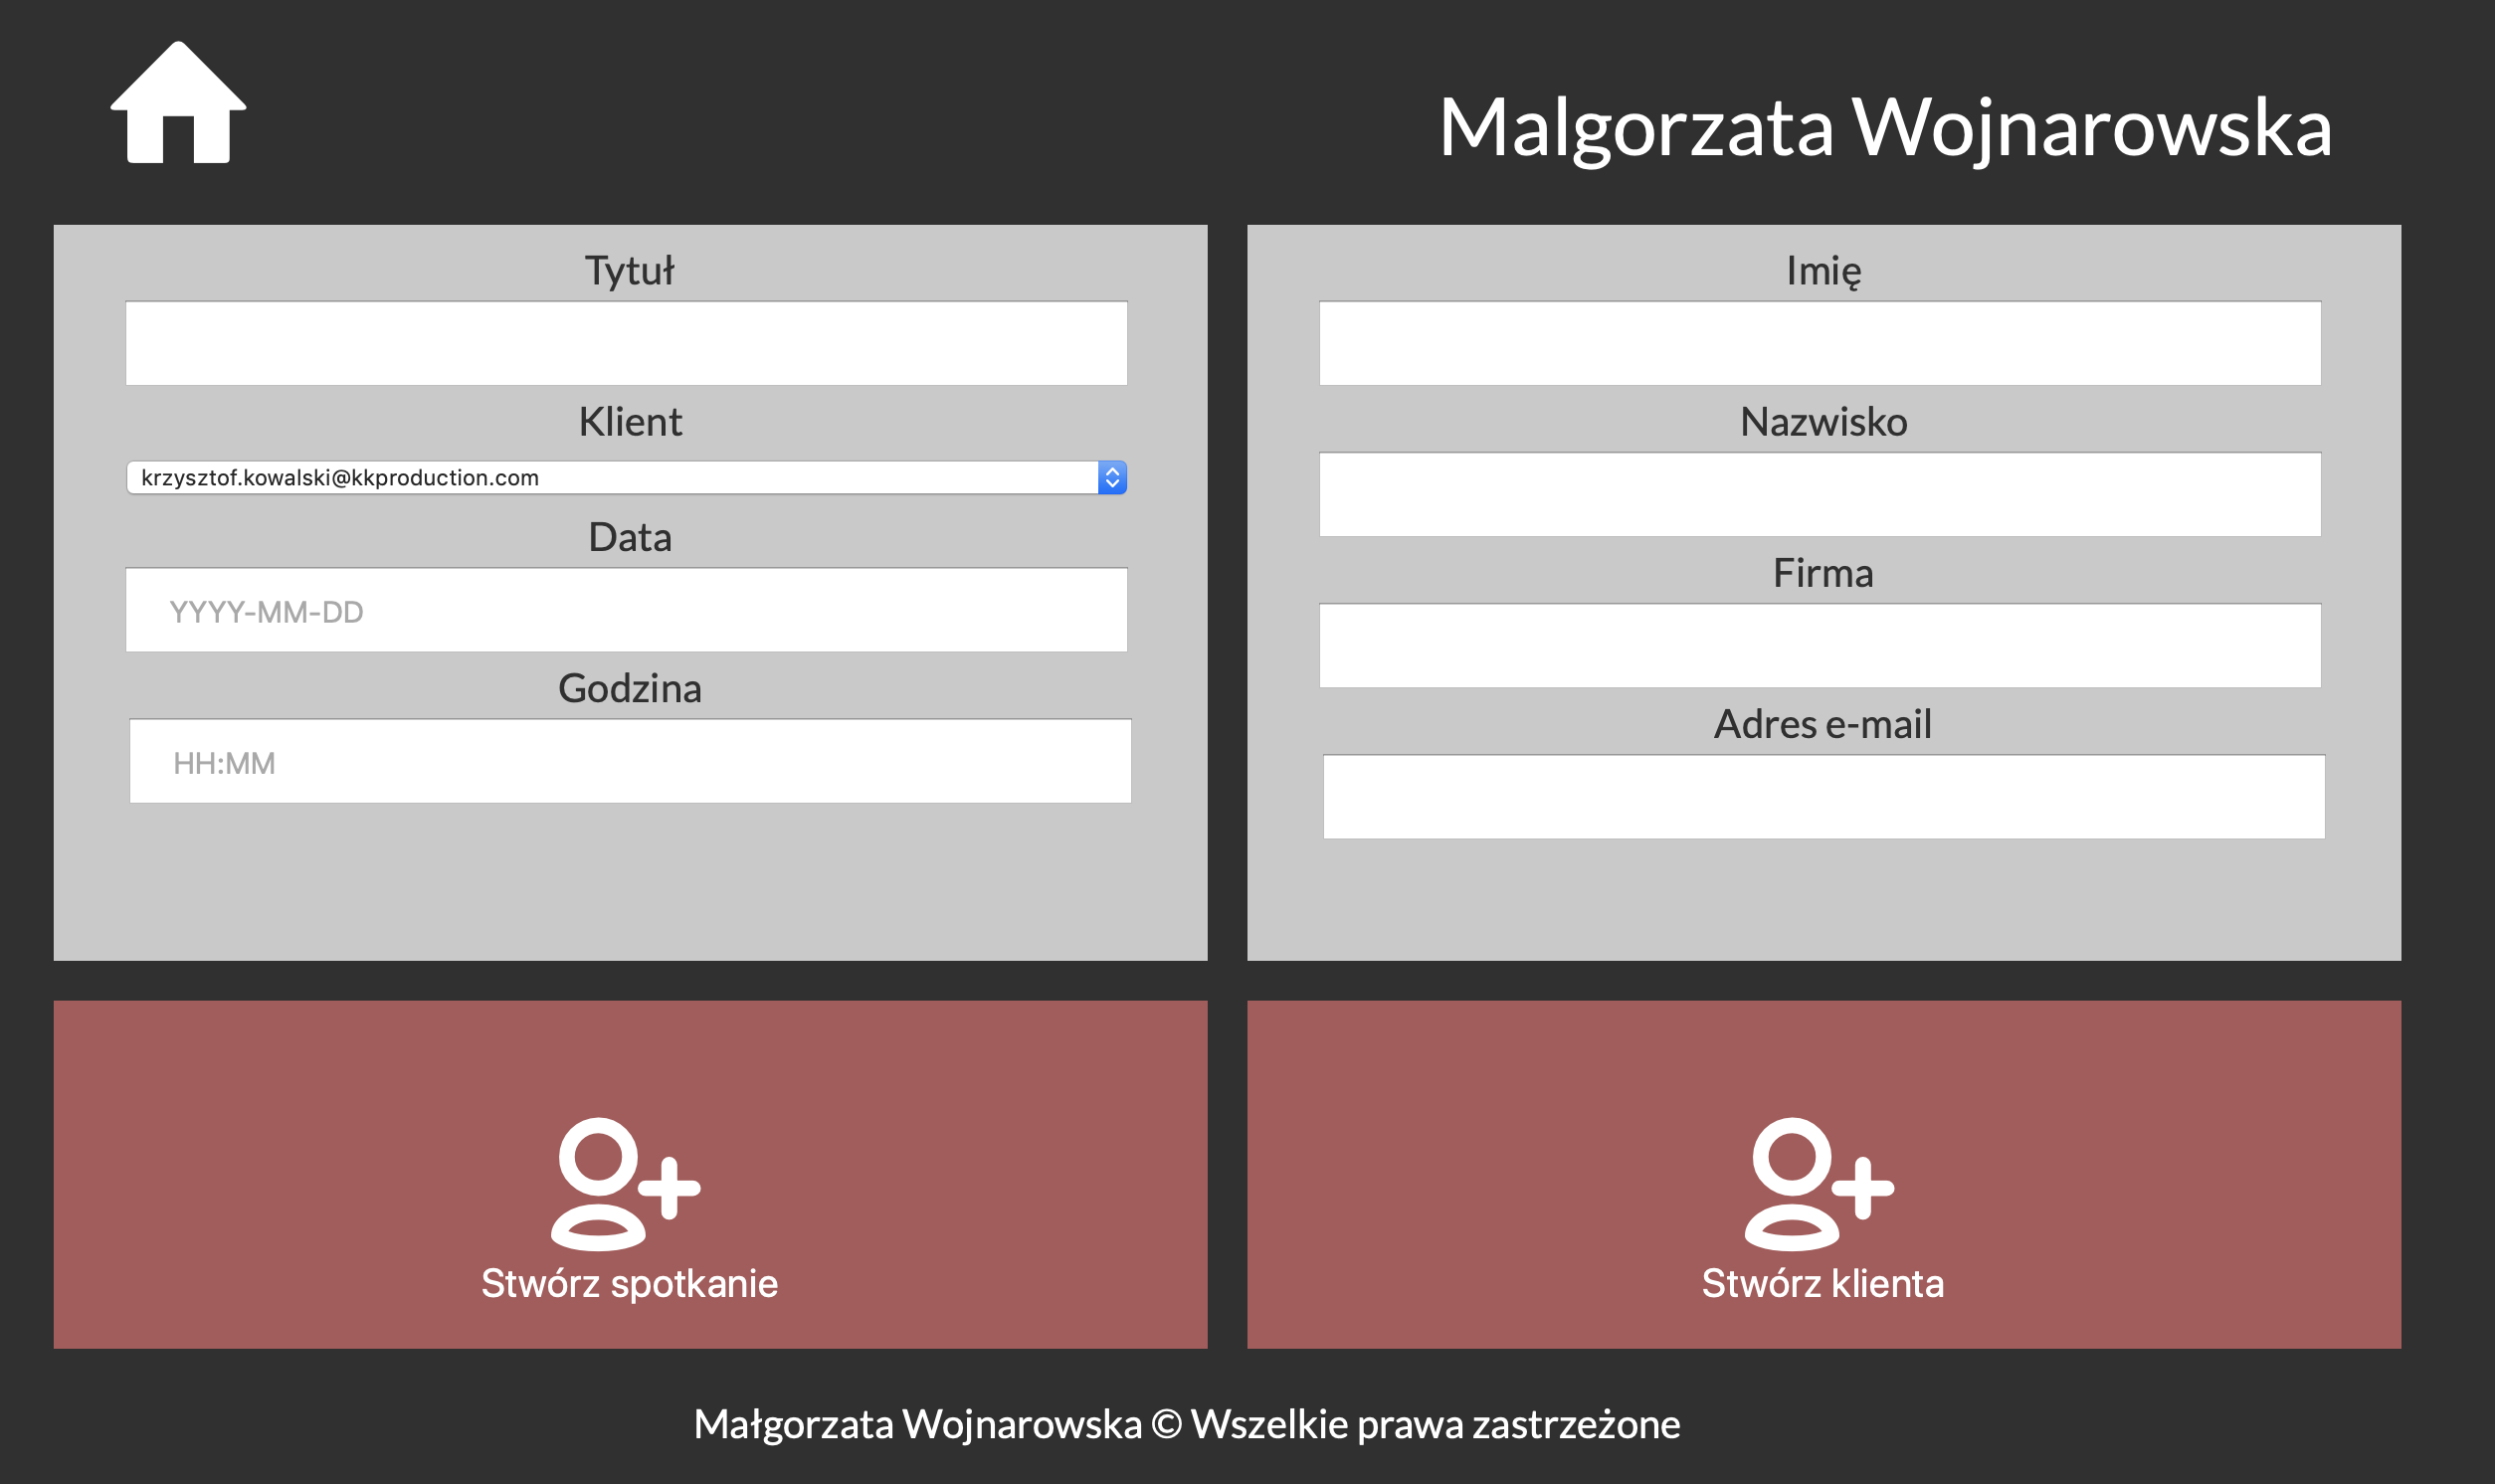
\includegraphics[width=0.75\textwidth]{dodaj_spotkanie}
		\caption{Dodawanie spotkania lub klienta}
		\label{fig:15}
	\end{figure}
	
	\begin{figure}[H]
		\centering
		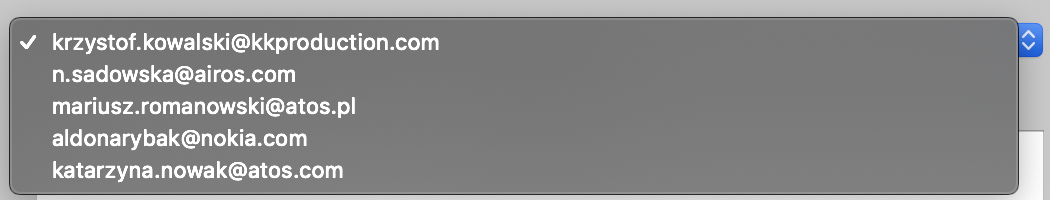
\includegraphics[width=0.75\textwidth]{wybor_klienta}
		\caption{Wybór klienta z listy rozwijanej}
		\label{fig:16}
	\end{figure}

	
	
	
	
	
	
	
\newpage
	
	
	
	
	

\subsection{Edycja/usuwanie notatki}

Spotkanie i notatki można edytować, a także usunąć. Notatki można przeglądać sortując je według dnia, miesiąca, roku, a także wybrać wszystkie, również takie, które nie mają przypisanej daty. Widok przy sortowaniu według miesiąca przedstawia Rysunek \ref{fig:17}. Po przejściu do wybranej notatki/spotkania, można na nią nacisnąć, aby wyświetlić szczegóły. Po naciśnięciu przycisku ’Edytuj’ pojawi się panel edycji (Rysunek \ref{fig:18}), gdzie możemy edytować wybraną notatkę, a następnie kliknąć przycisk ’Zapisz’, aby ją nadpisać lub 'Usuń', aby całkowicie ją usunąć.

	\begin{figure}[H]
		\centering
		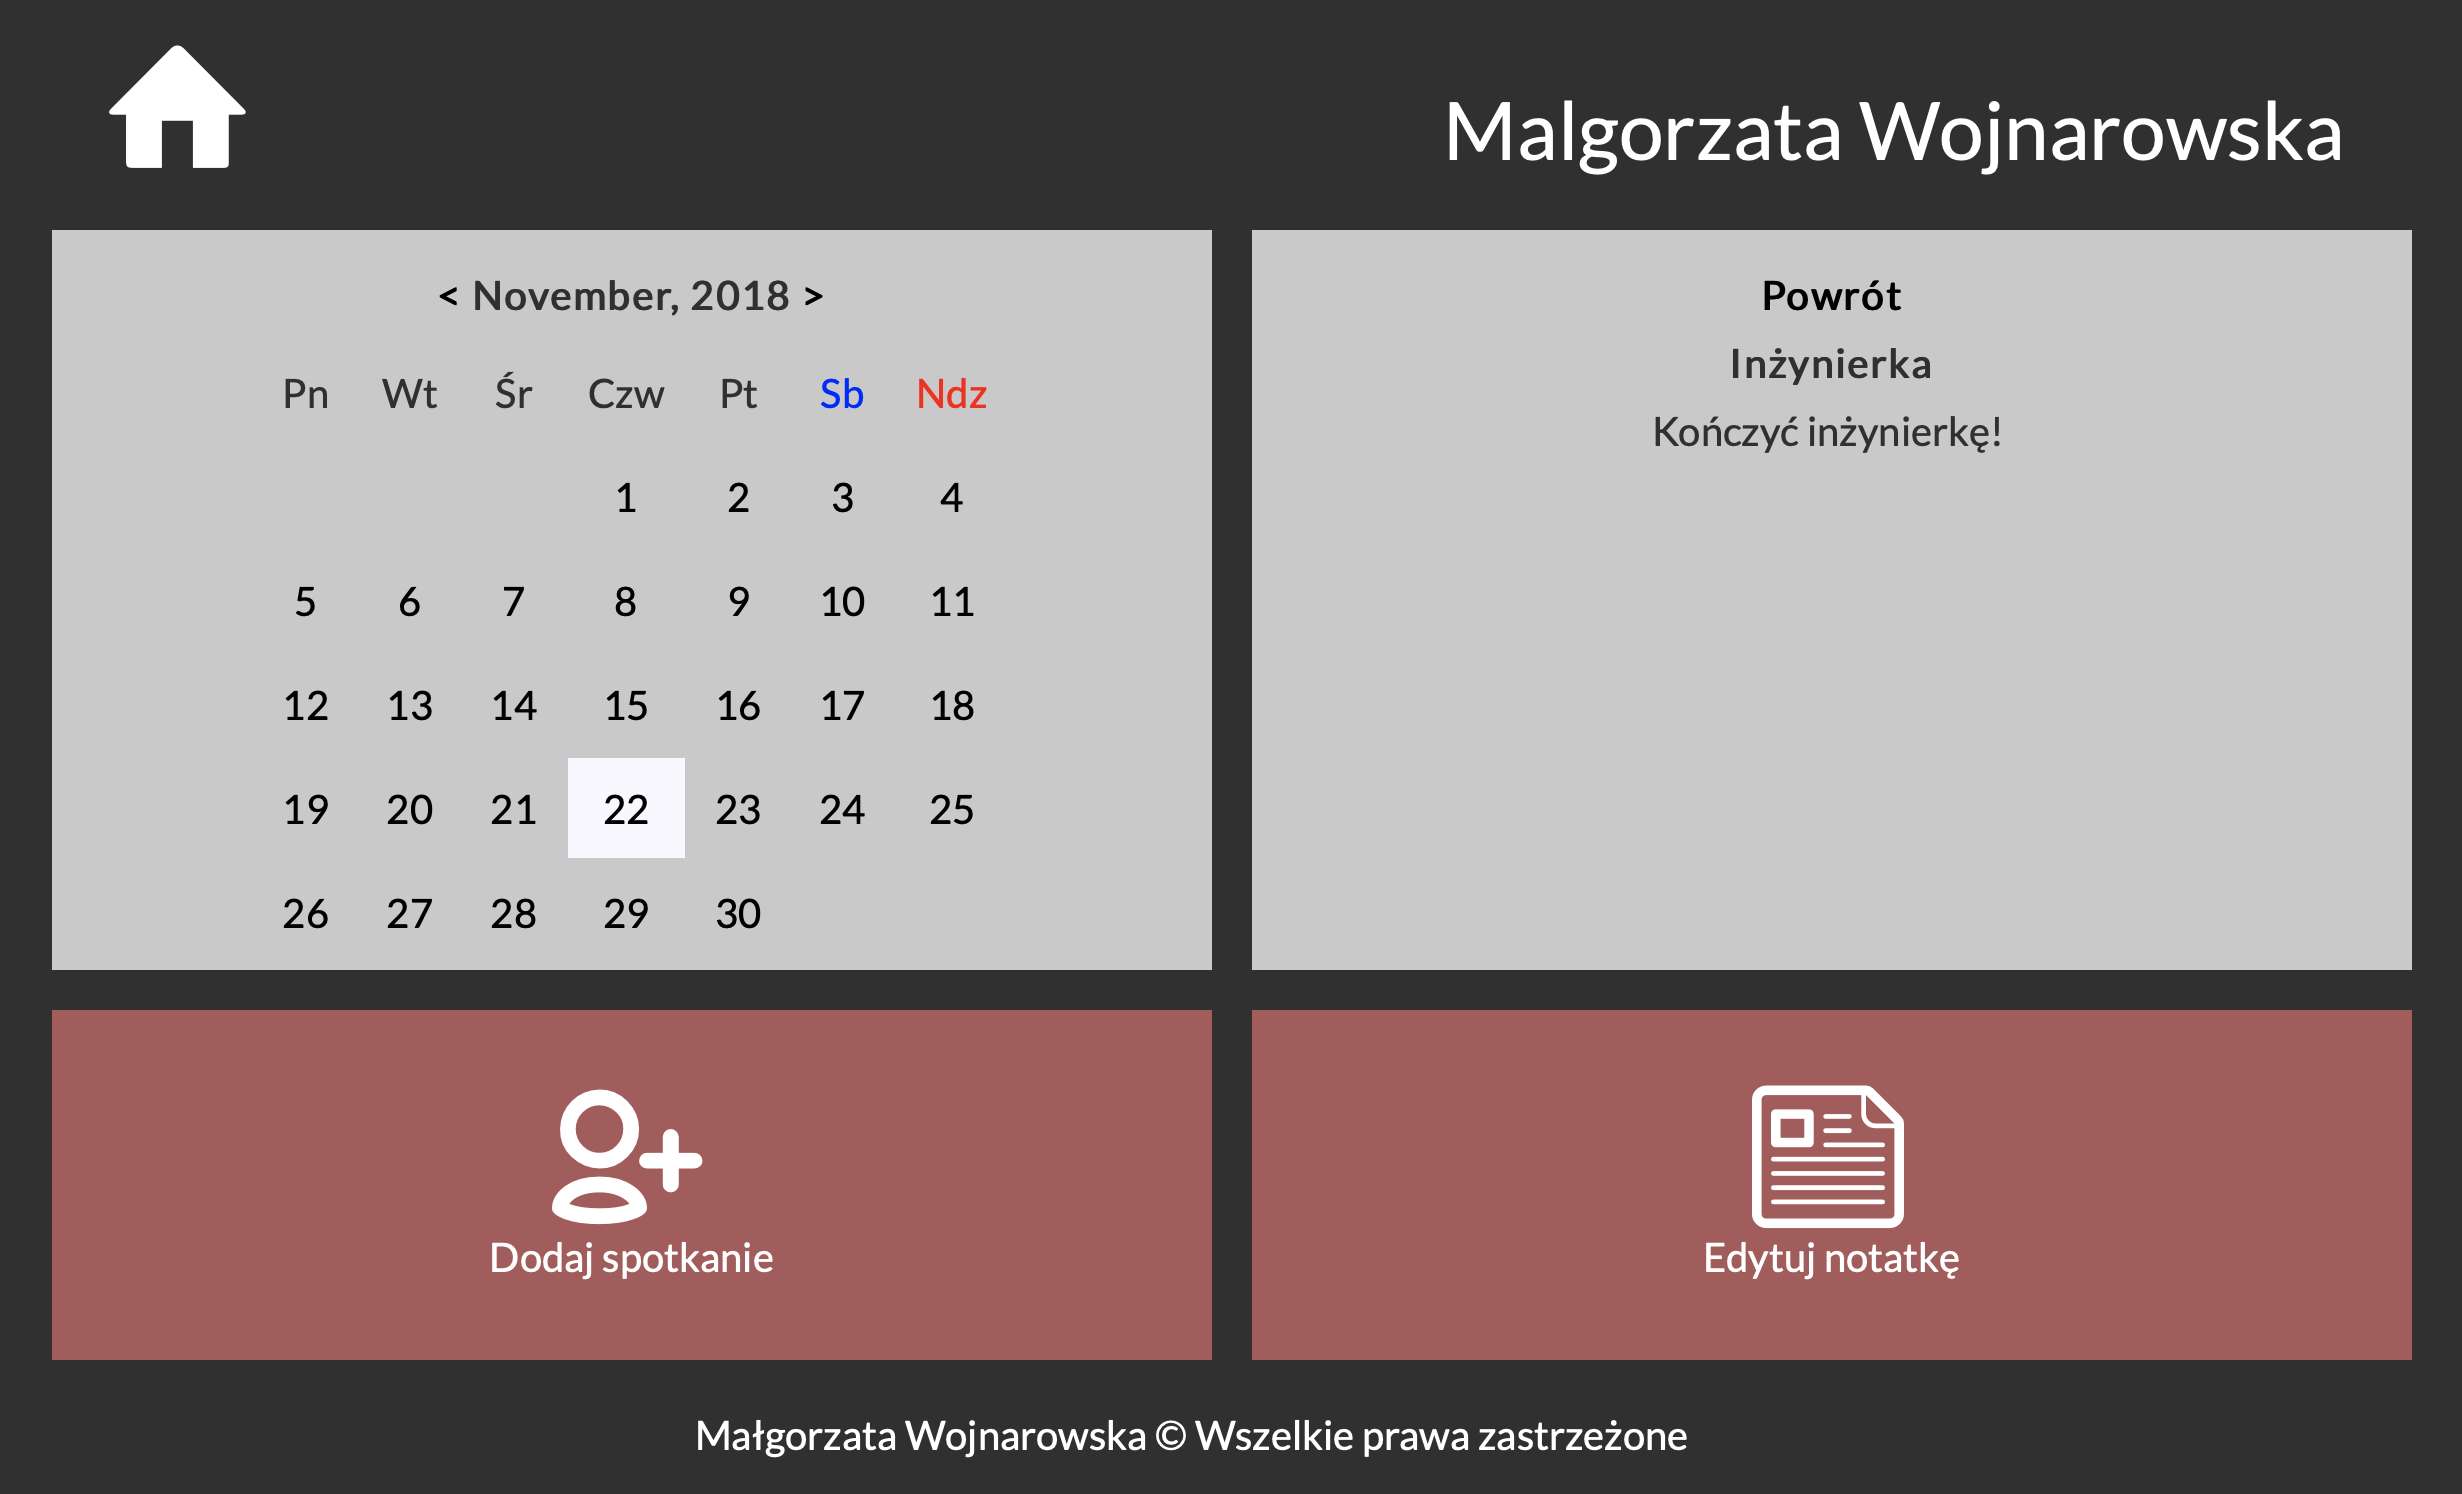
\includegraphics[width=0.75\textwidth]{miesiac_notatka}
		\caption{Widok miesiąca po wybraniu konkretnej notatki}
		\label{fig:17}
	\end{figure}
	
	
	\begin{figure}[H]
		\centering
		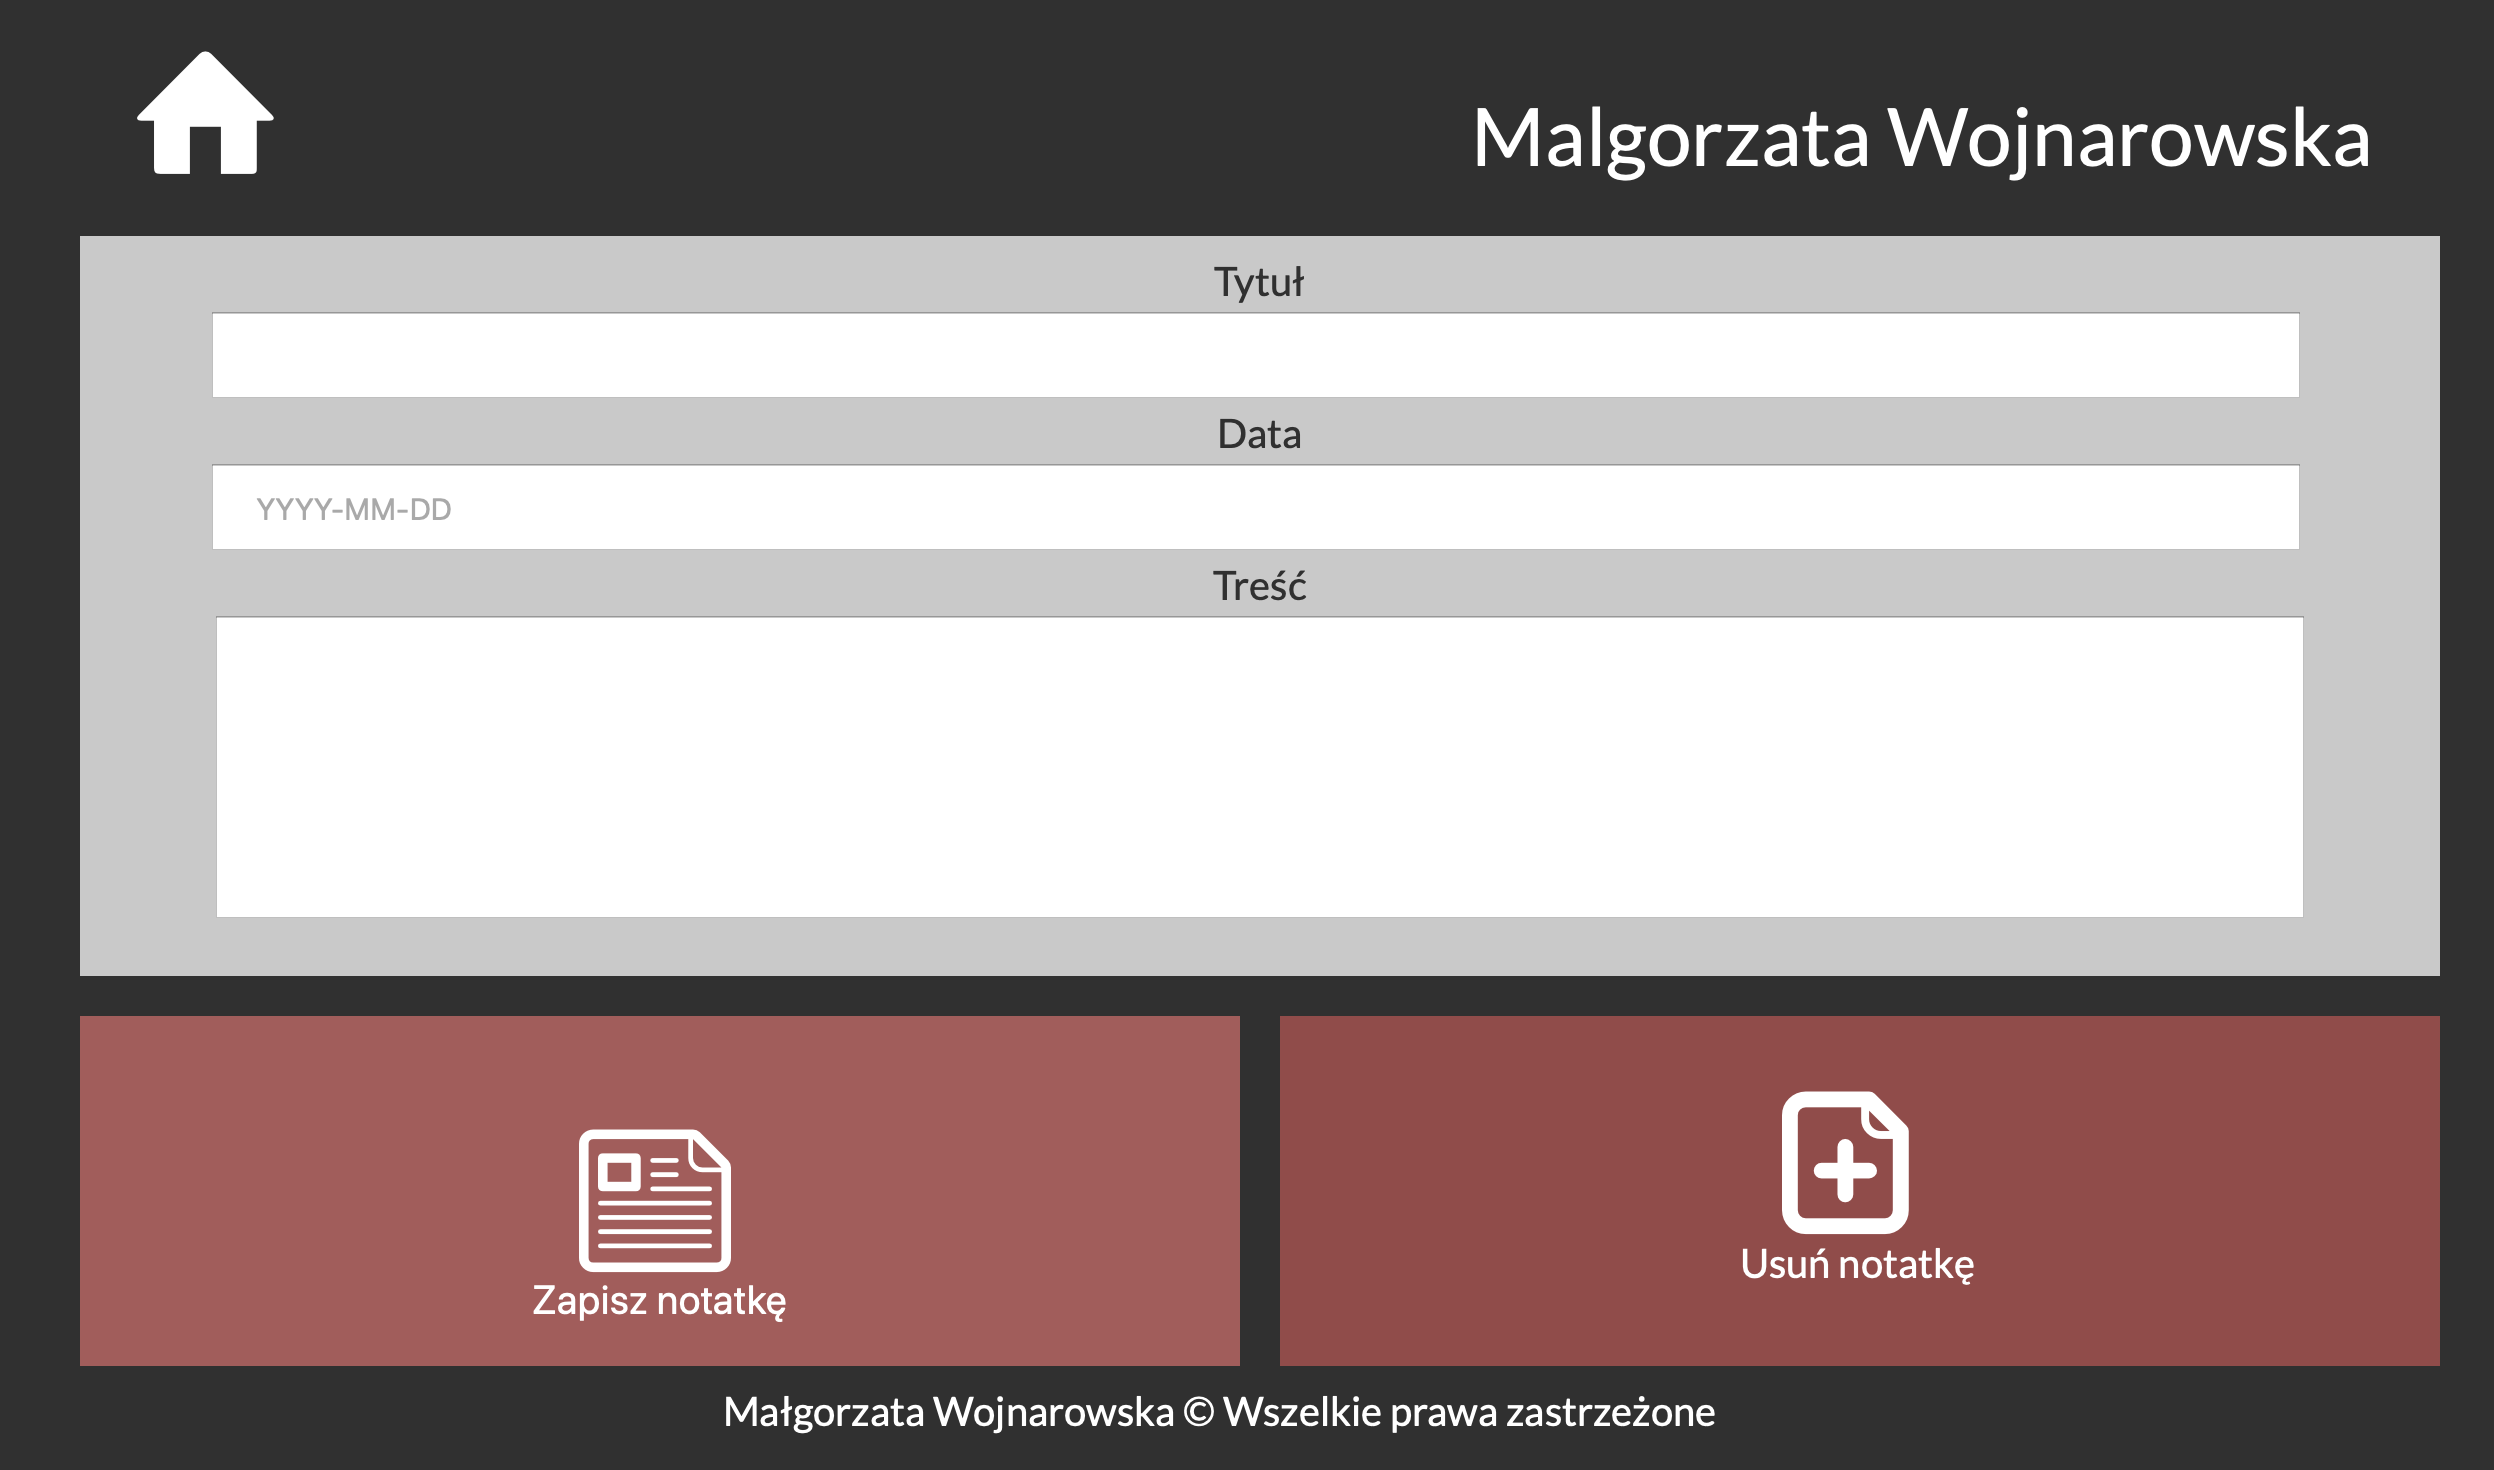
\includegraphics[width=0.75\textwidth]{edycja_notatka}
		\caption{Panel edycji i usuwania notatki}
		\label{fig:18}
	\end{figure}
	
	
	
	
	
\newpage
	
	
	
	
	

\subsection{Rejestracja użytkownika}

Każdy nowy użytkownik ma możliwość rejestracji w aplikacji. Aby się zarejestrować należy wejść w panel logowania, a następnie nacisnąć przycisk 'Zarejestruj się'. Po wykonaniu tej czynności pojawi się formularz rejestracji (Rysunek \ref{fig:19}). Po prawidłowym wypełnieniu formularza zostanie on przekierowany do strony, która informuje go, że został on zarejestrowany poprawnie i od tej pory ma on możliwość zalogowania się w systemie (Rysunek \ref{fig:20}).

	\begin{figure}[H]
		\centering
		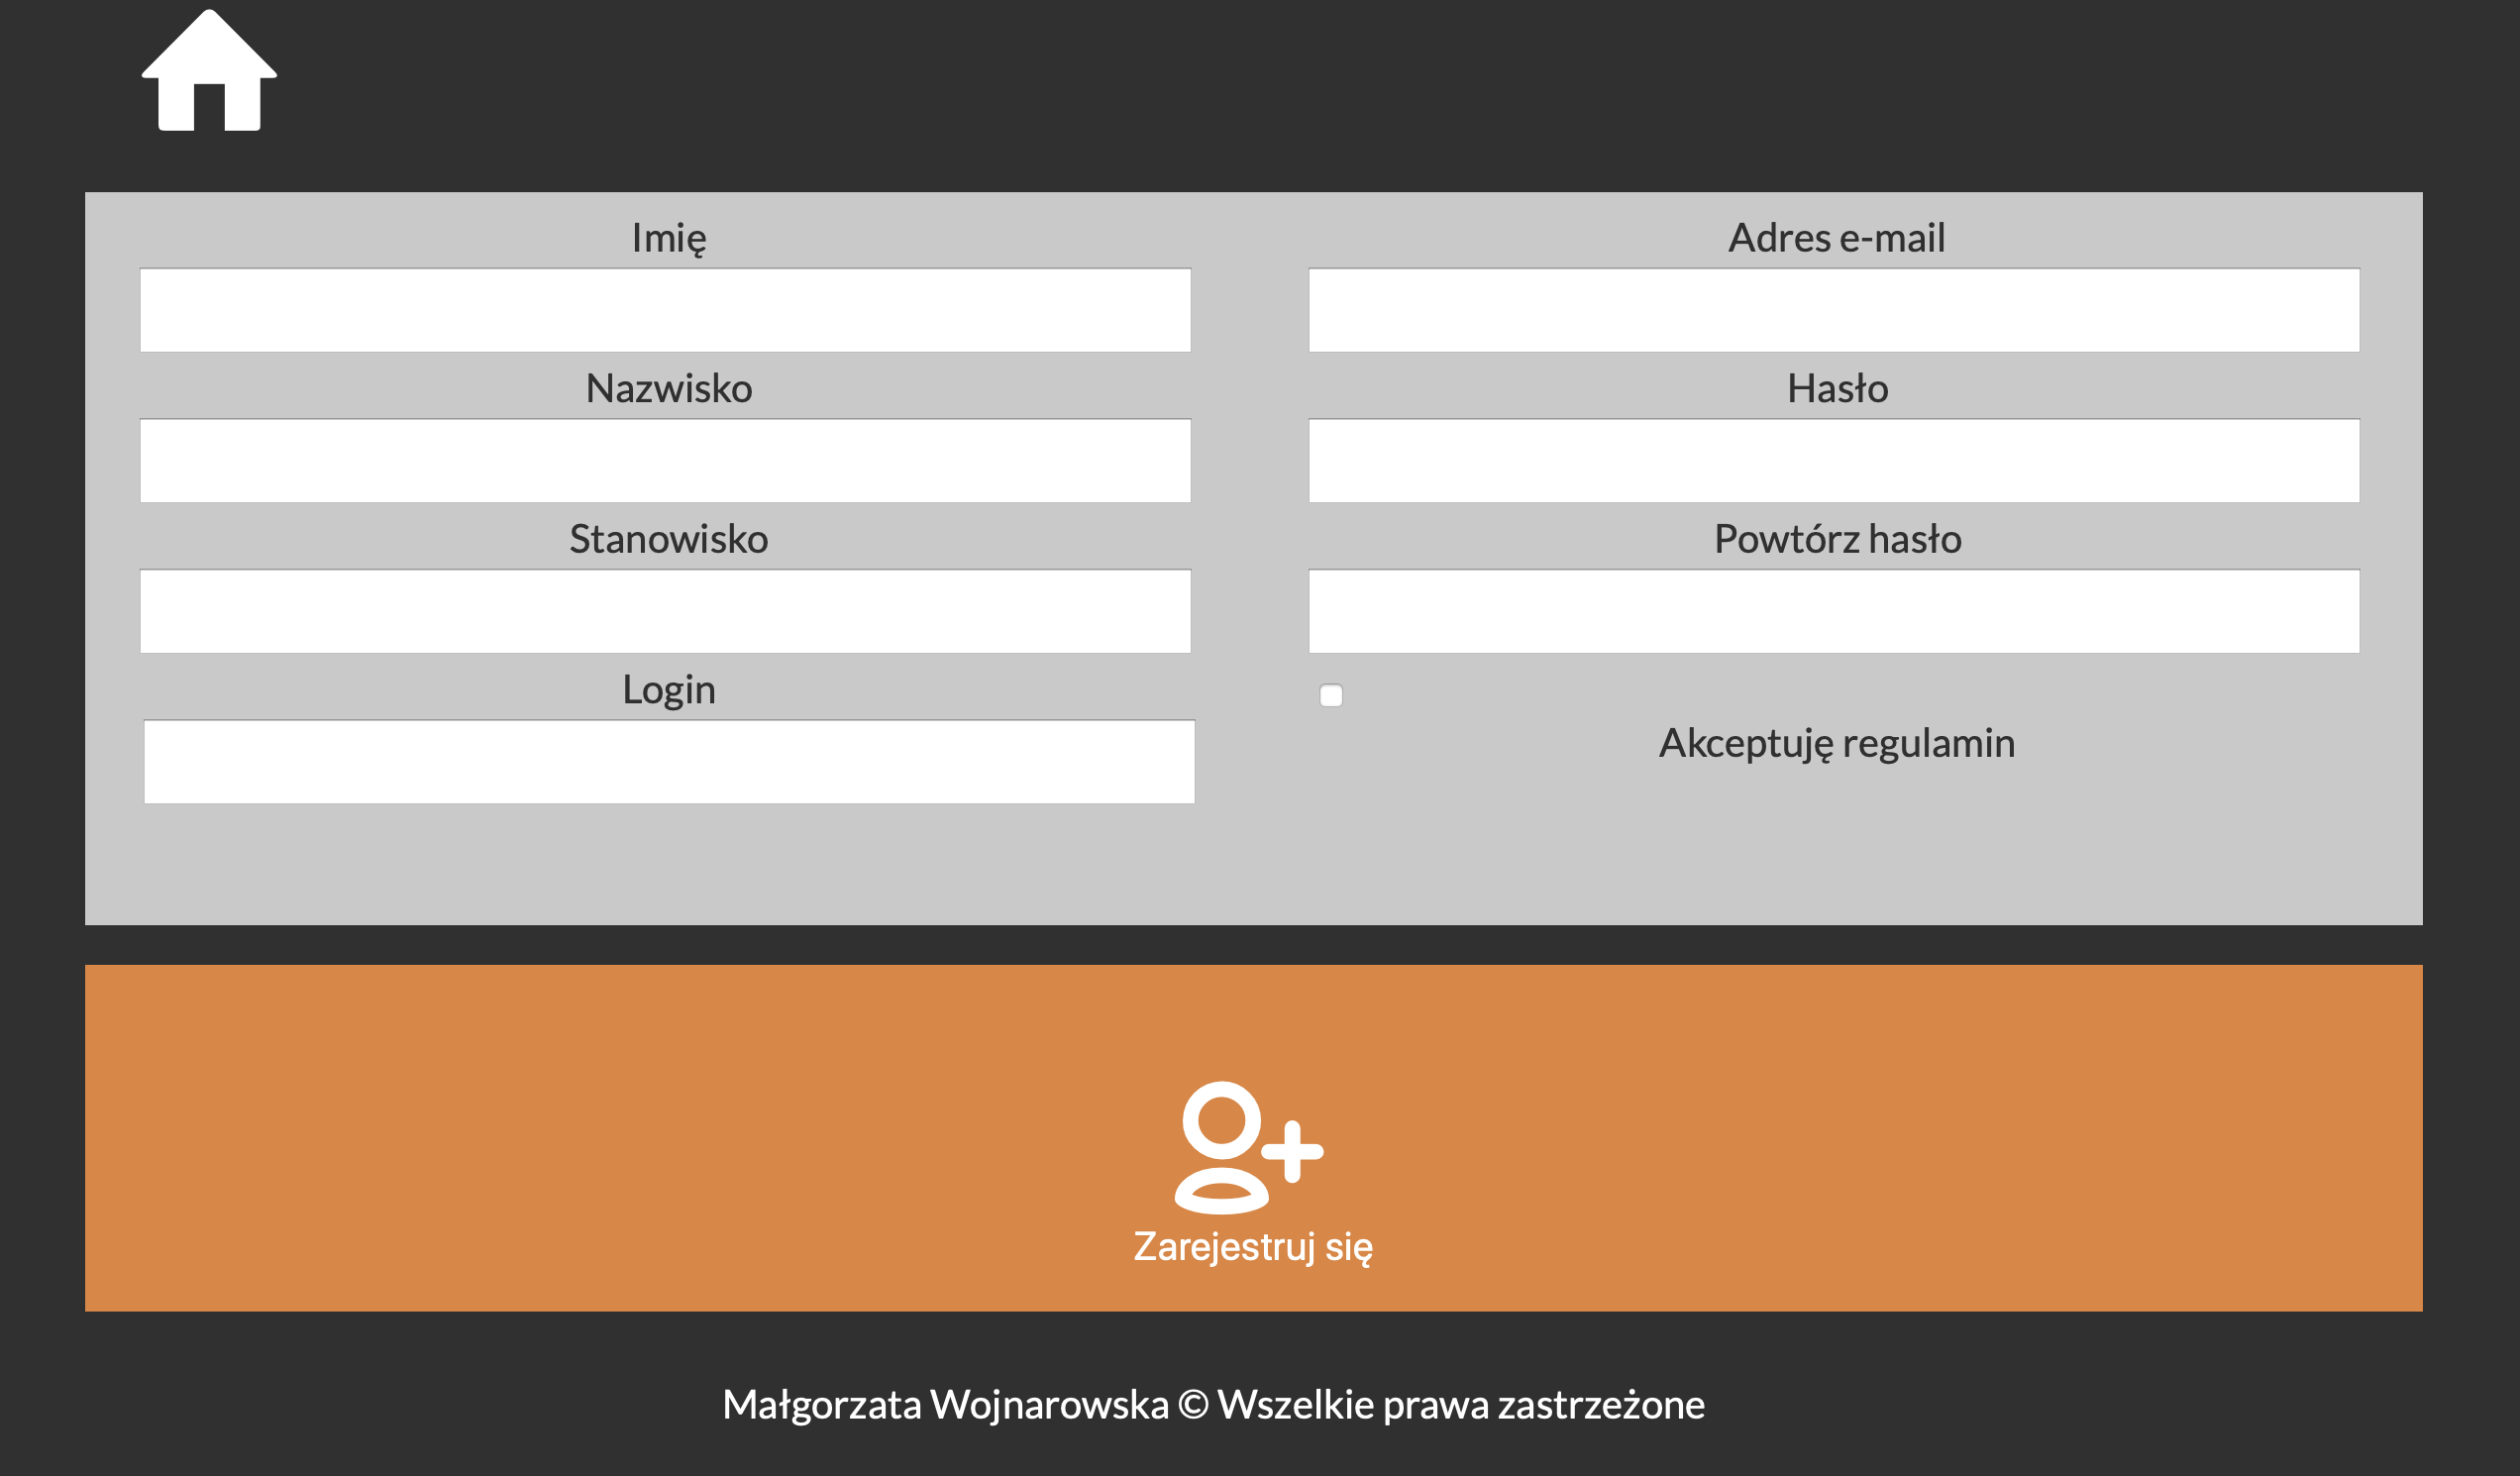
\includegraphics[width=0.75\textwidth]{rejestracja}
		\caption{Rejestracja nowego użytkownika}
		\label{fig:19}
	\end{figure}
	
	\begin{figure}[H]
		\centering
		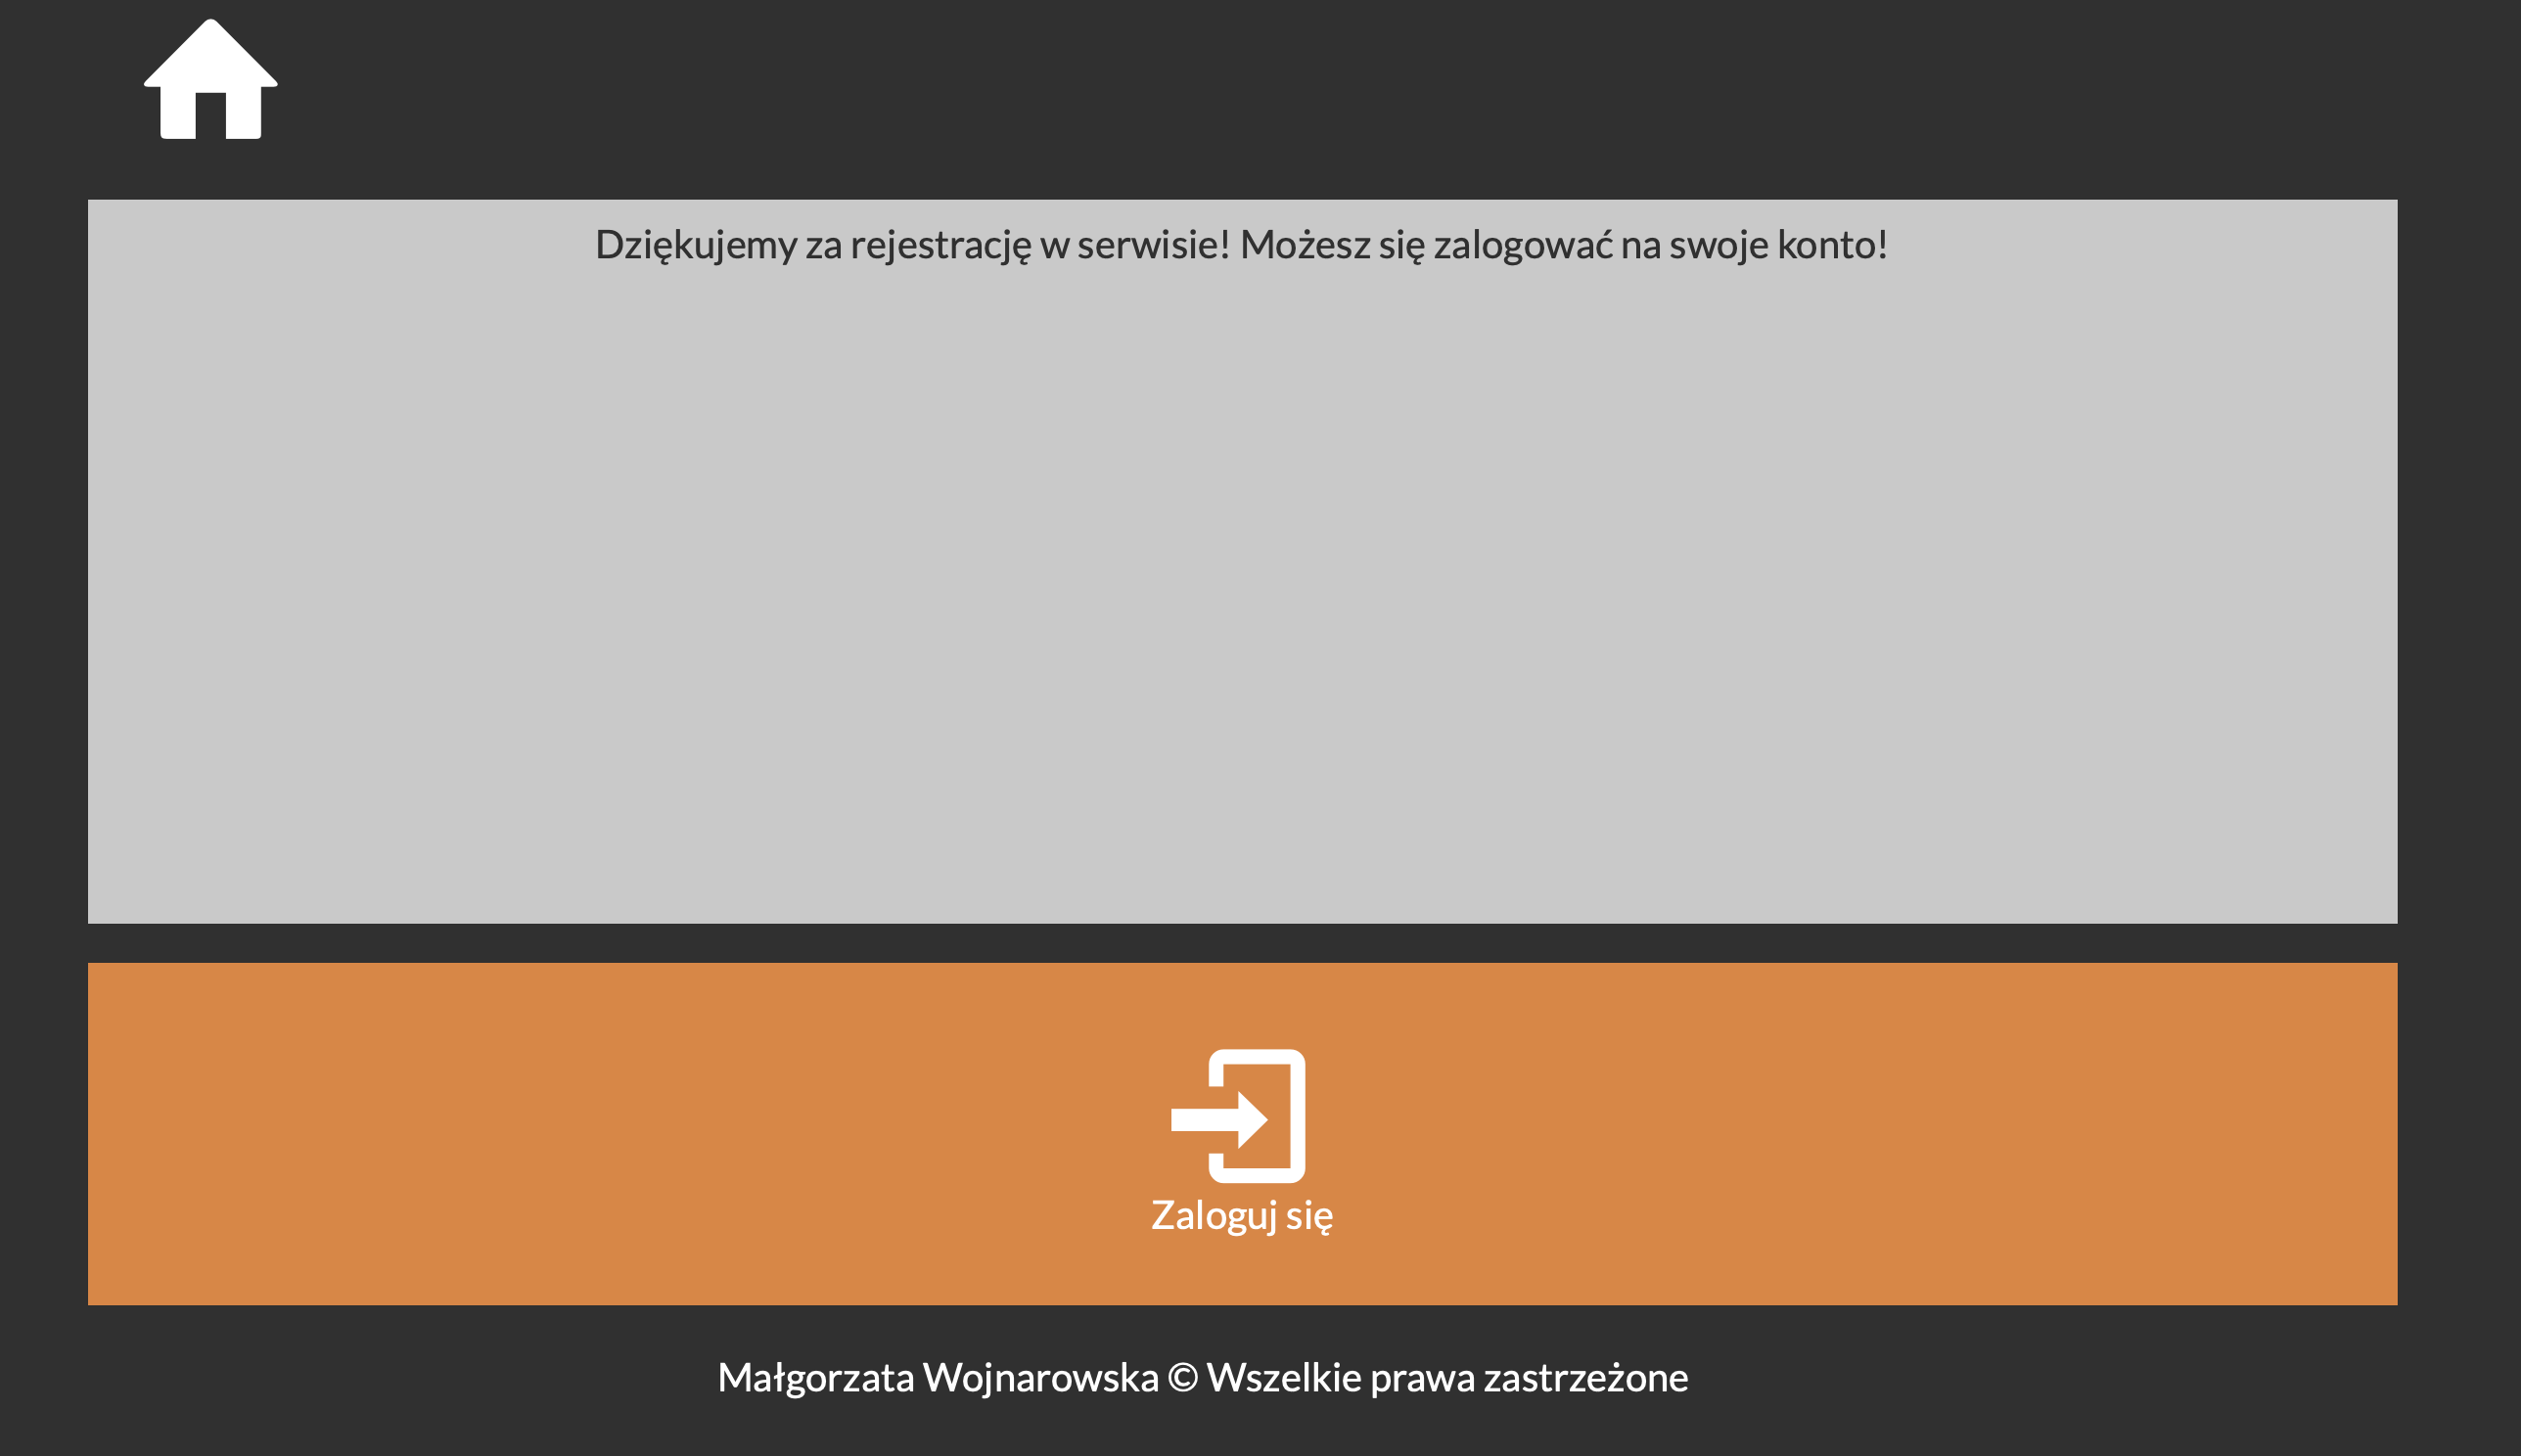
\includegraphics[width=0.75\textwidth]{udana_rejestracja}
		\caption{Ekran po udanej rejestracji}
		\label{fig:20}
	\end{figure}
	
		
	
	
\newpage
	
	
	
	


\subsection{Przeglądanie zaplanowanych spotkań oraz notatek}
 
Wszystkie notatki oraz spotkania można przeglądać dowolnie, sortując je na dany dzień (Rysunek \ref{fig:21}), miesiąc (Rysunek \ref{fig:22}) oraz rok (Rysunek \ref{fig:23}). Można także wyświetlić wszystkie notatki niezależnie od daty. Dni, miesiące i lata można przewijać za pomocą strzałek umieszczonych przy dacie. Po naciśnięciu na dany miesiąc w zakładce 'Rok' zostaniemy przeniesieni do danego miesiąca, a po kliknięciu w konkretny dzień - do widoku aplikacji i zaplanowanych czynności na ten dzień. Bieżący dzień jest podświetlany, co widać na Rysunku \ref{fig:22}.

	\begin{figure}[H]
		\centering
		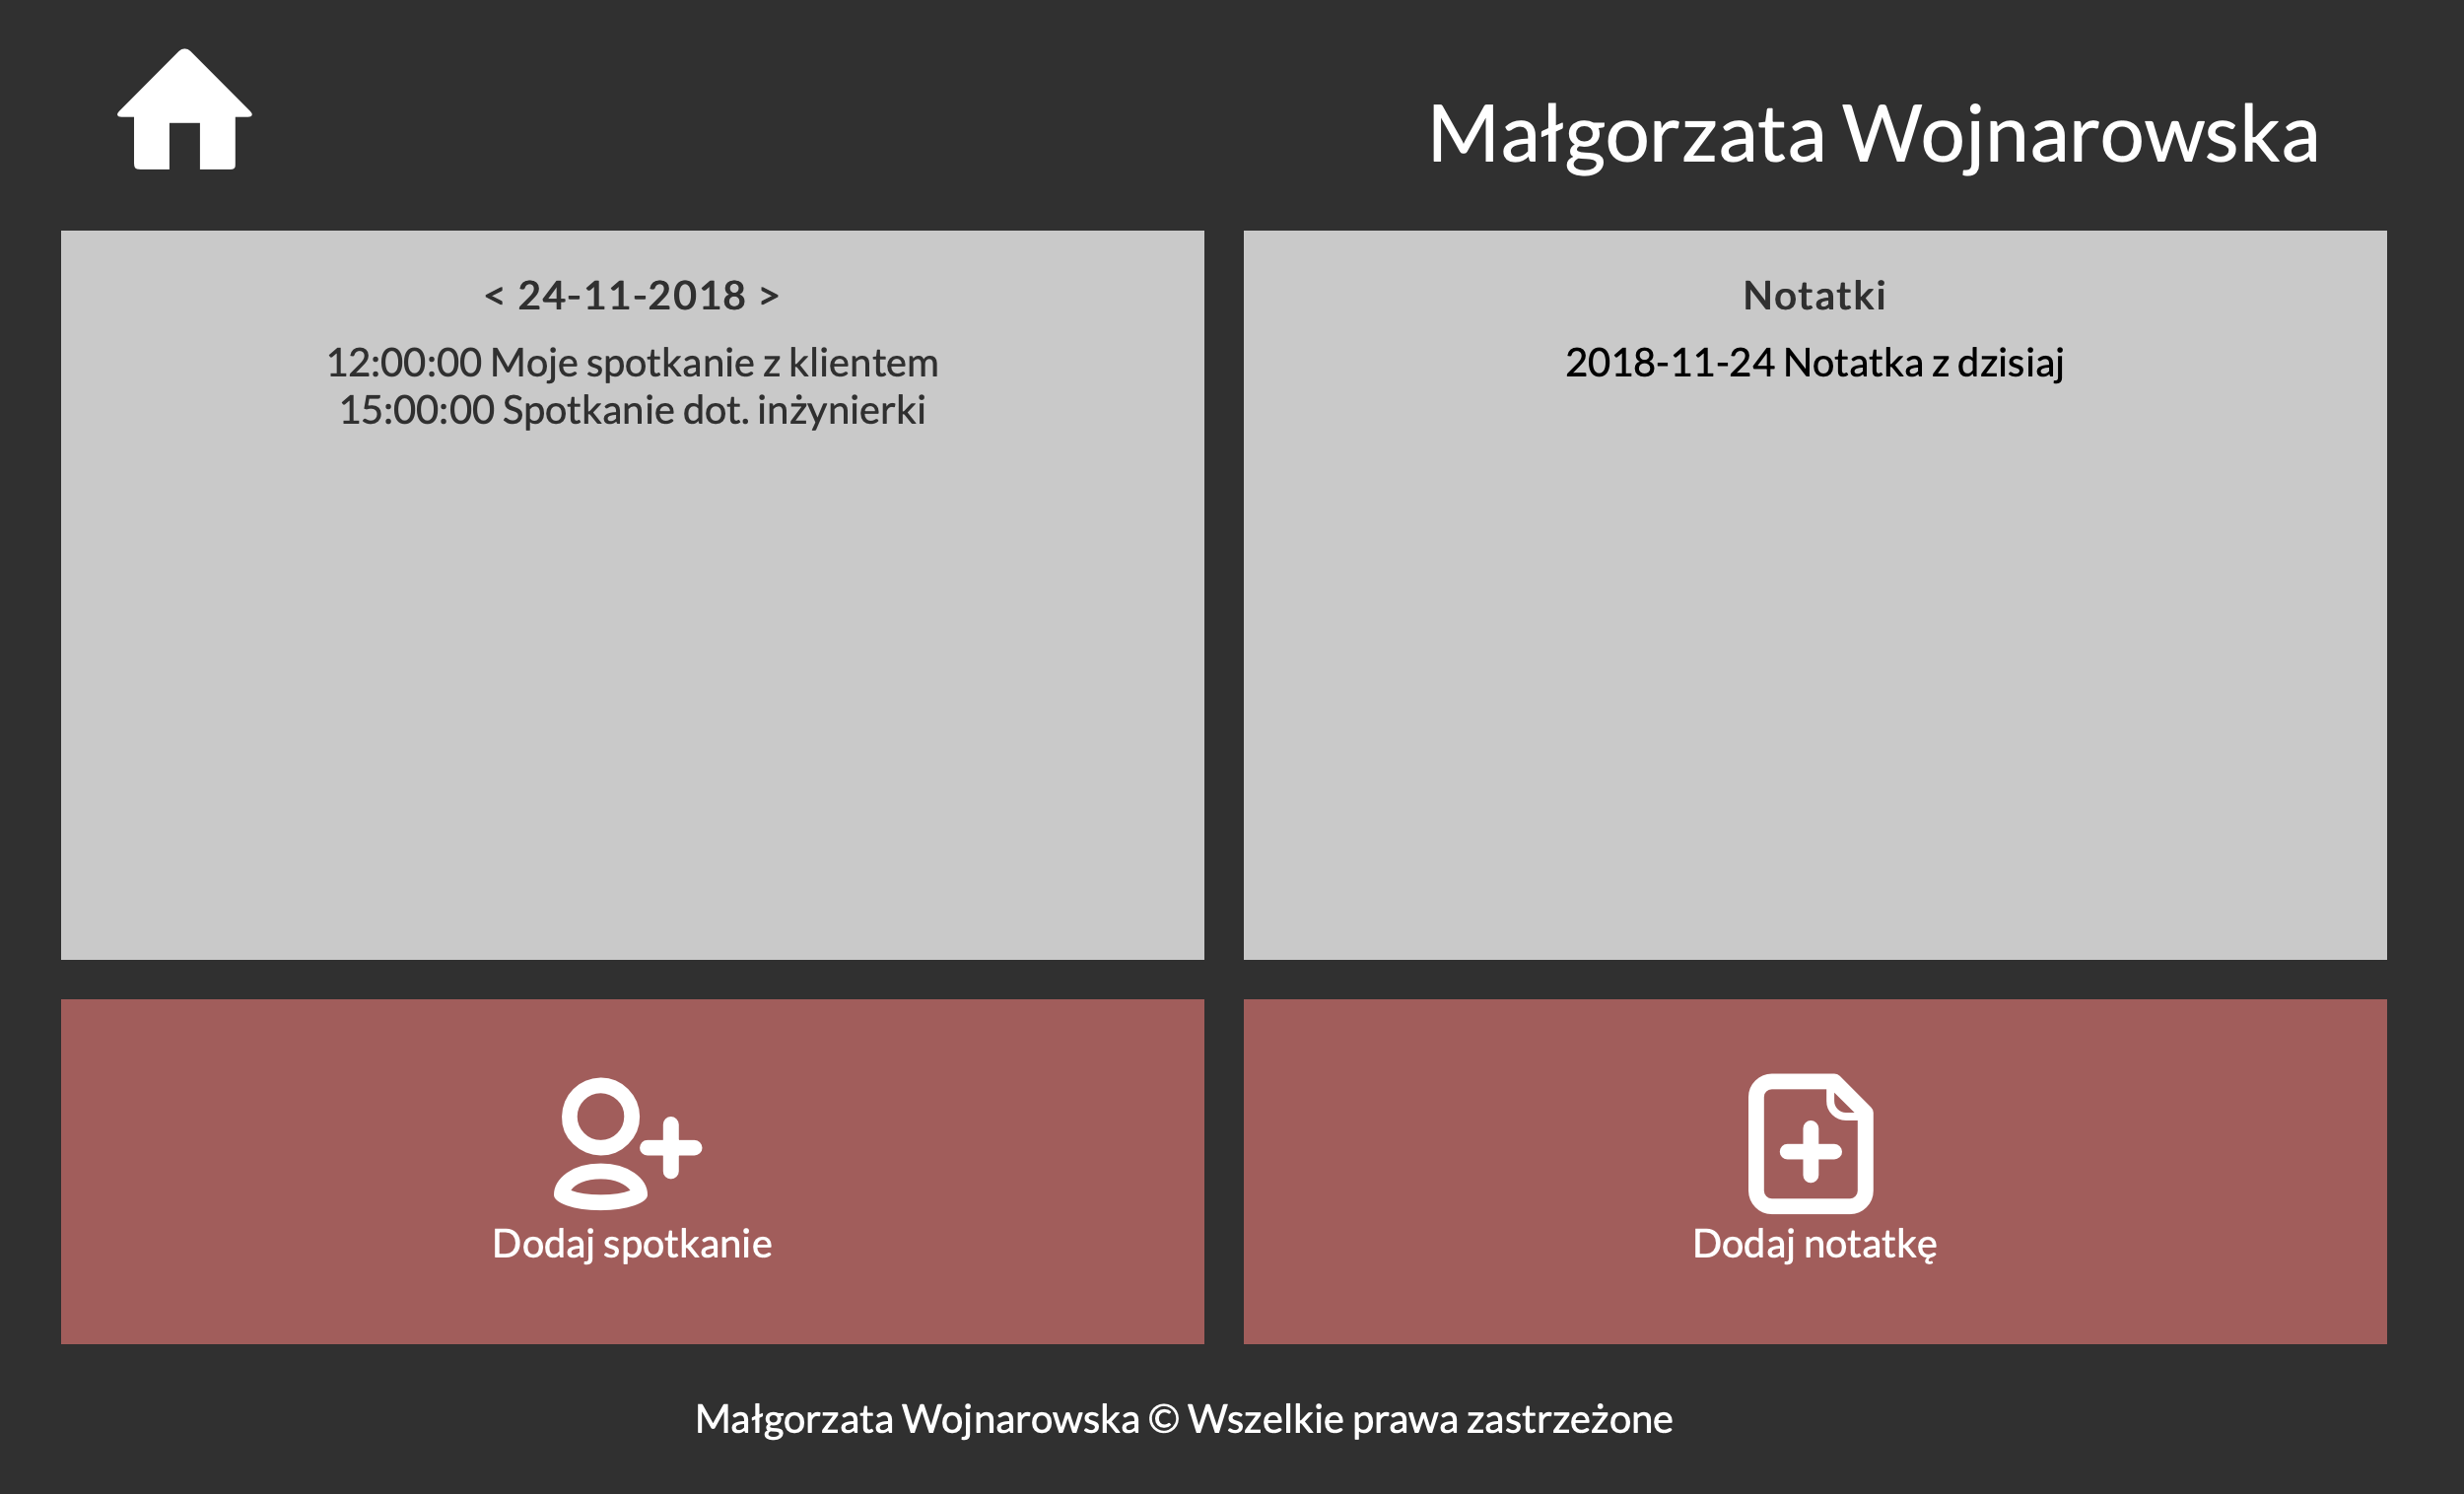
\includegraphics[width=0.75\textwidth]{day}
		\caption{Widok bieżącego dnia}
		\label{fig:21}
	\end{figure}

	\begin{figure}[H]
		\centering
		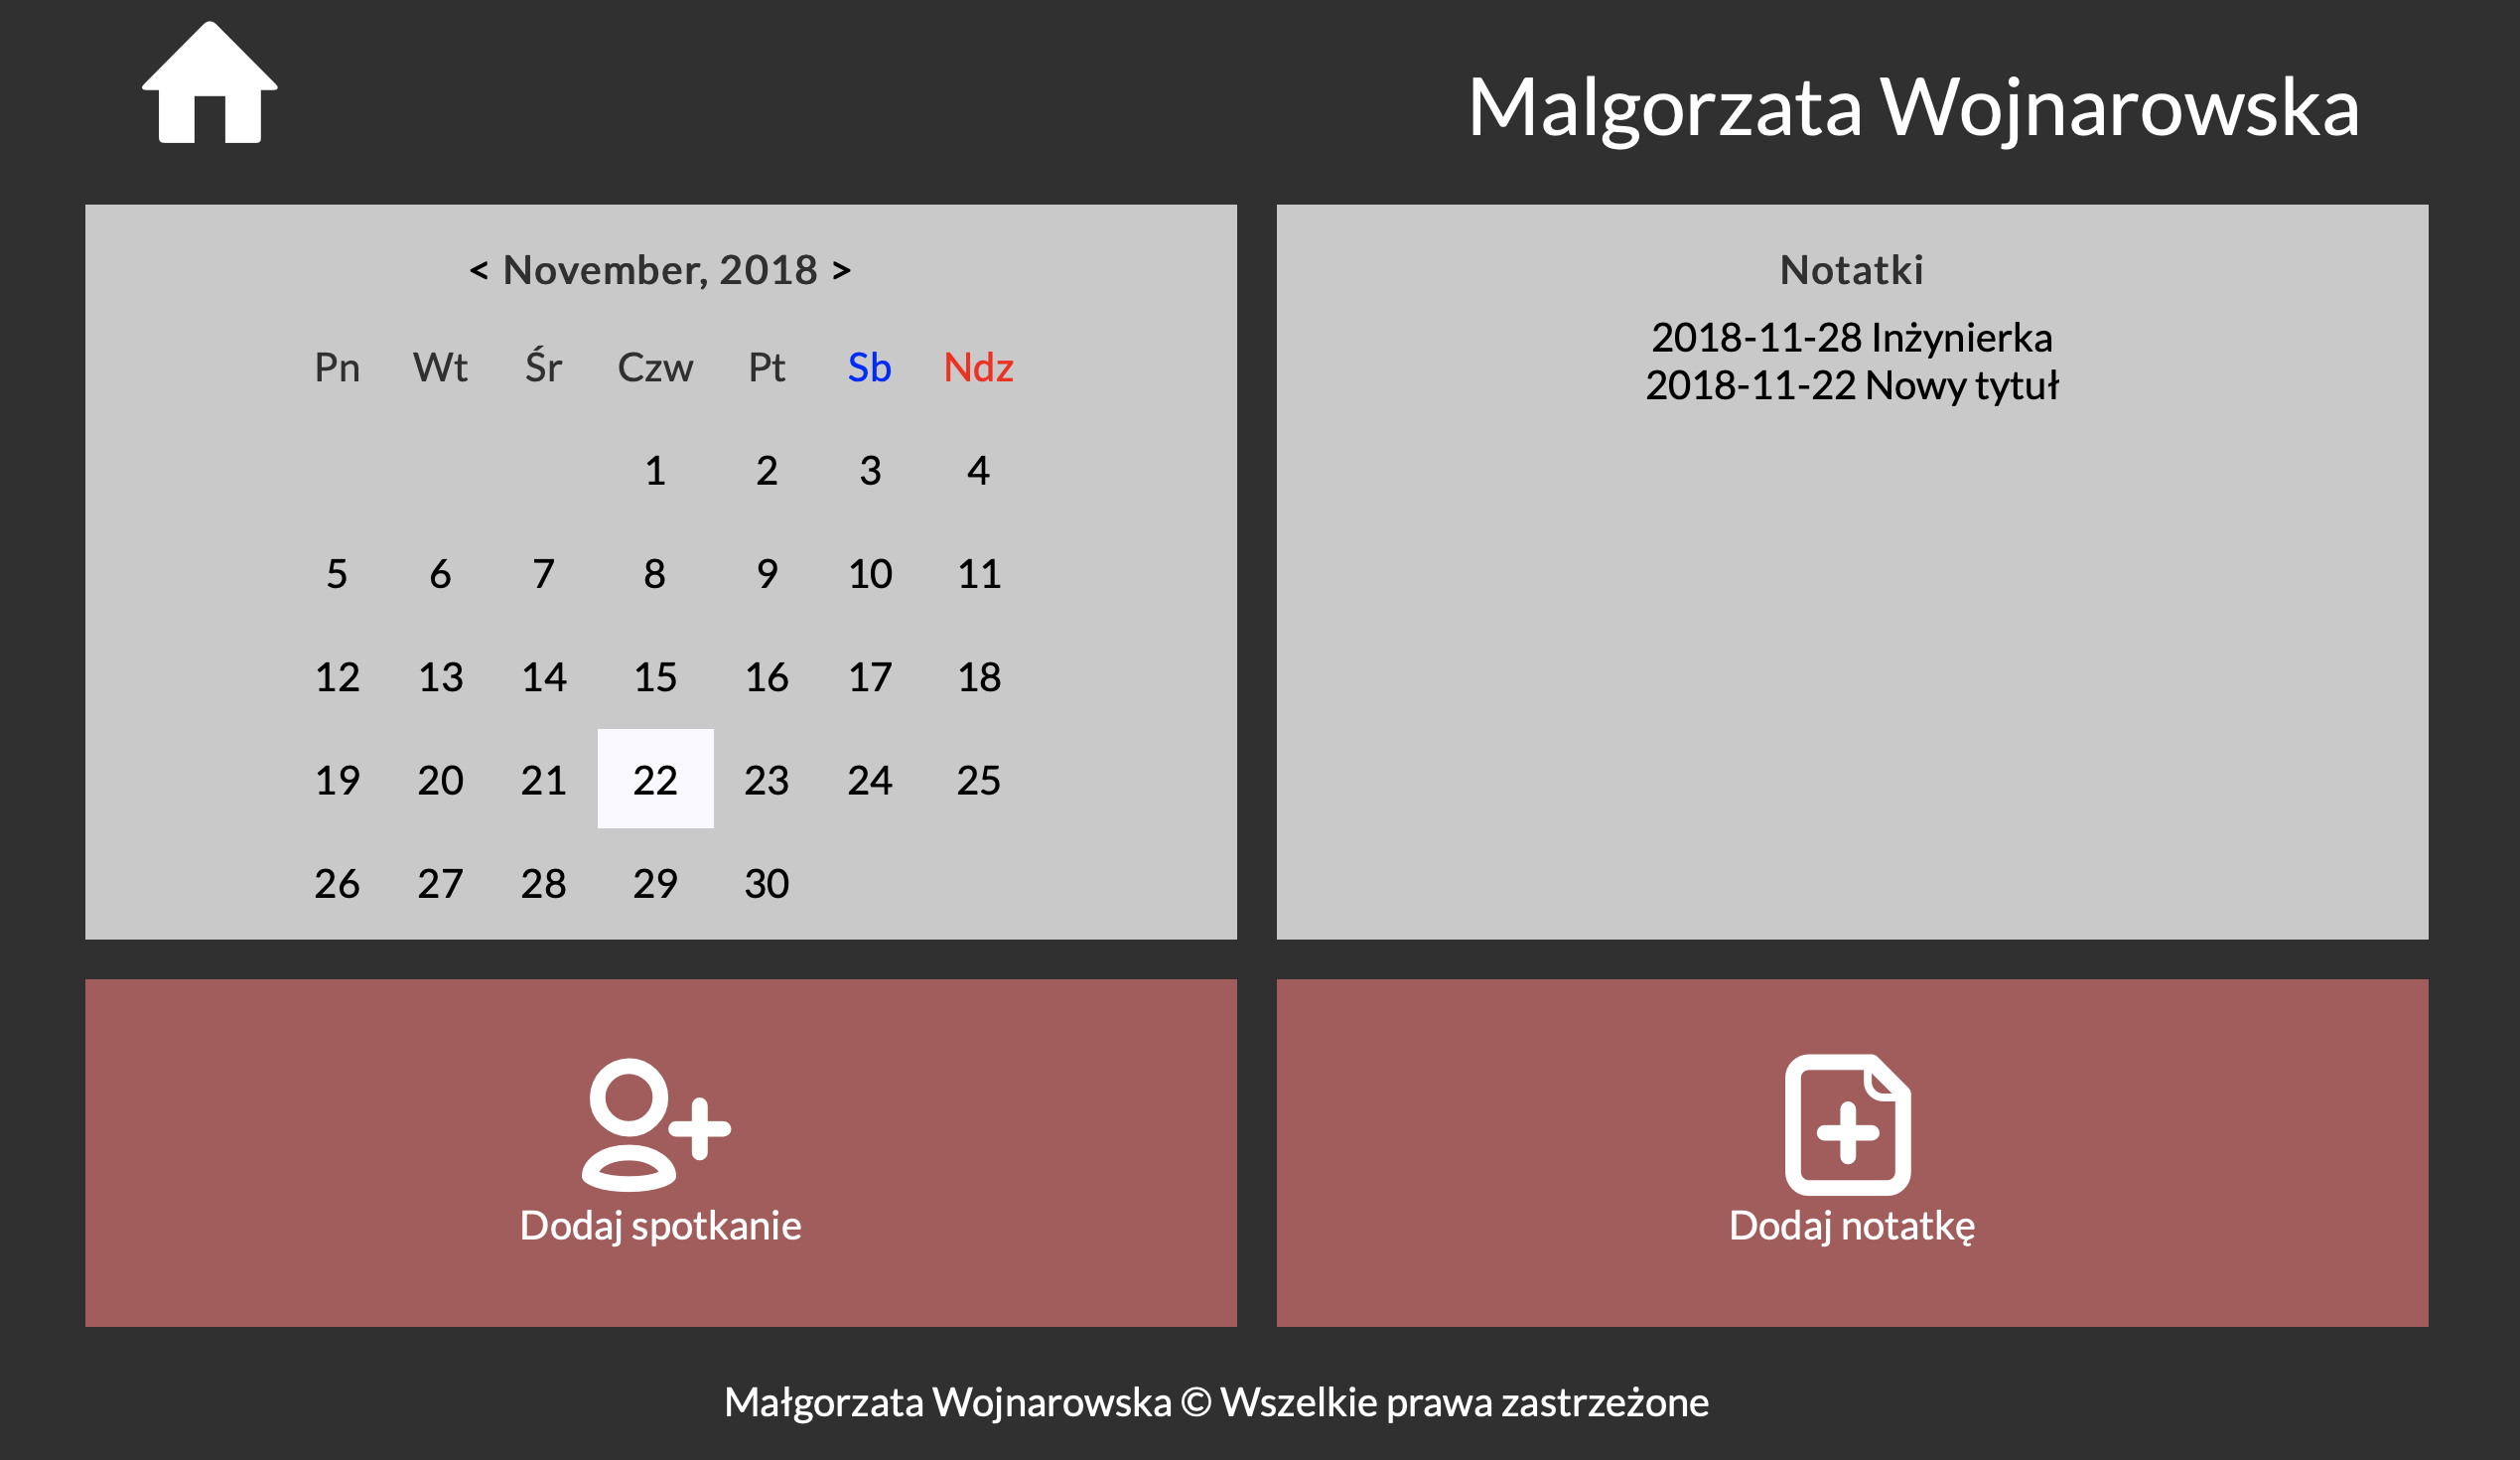
\includegraphics[width=0.75\textwidth]{miesiac}
		\caption{Widok bieżącego miesiąca z zaznaczoną aktualnie datą}
		\label{fig:22}
	\end{figure}
	
	
	\begin{figure}[H]
		\centering
		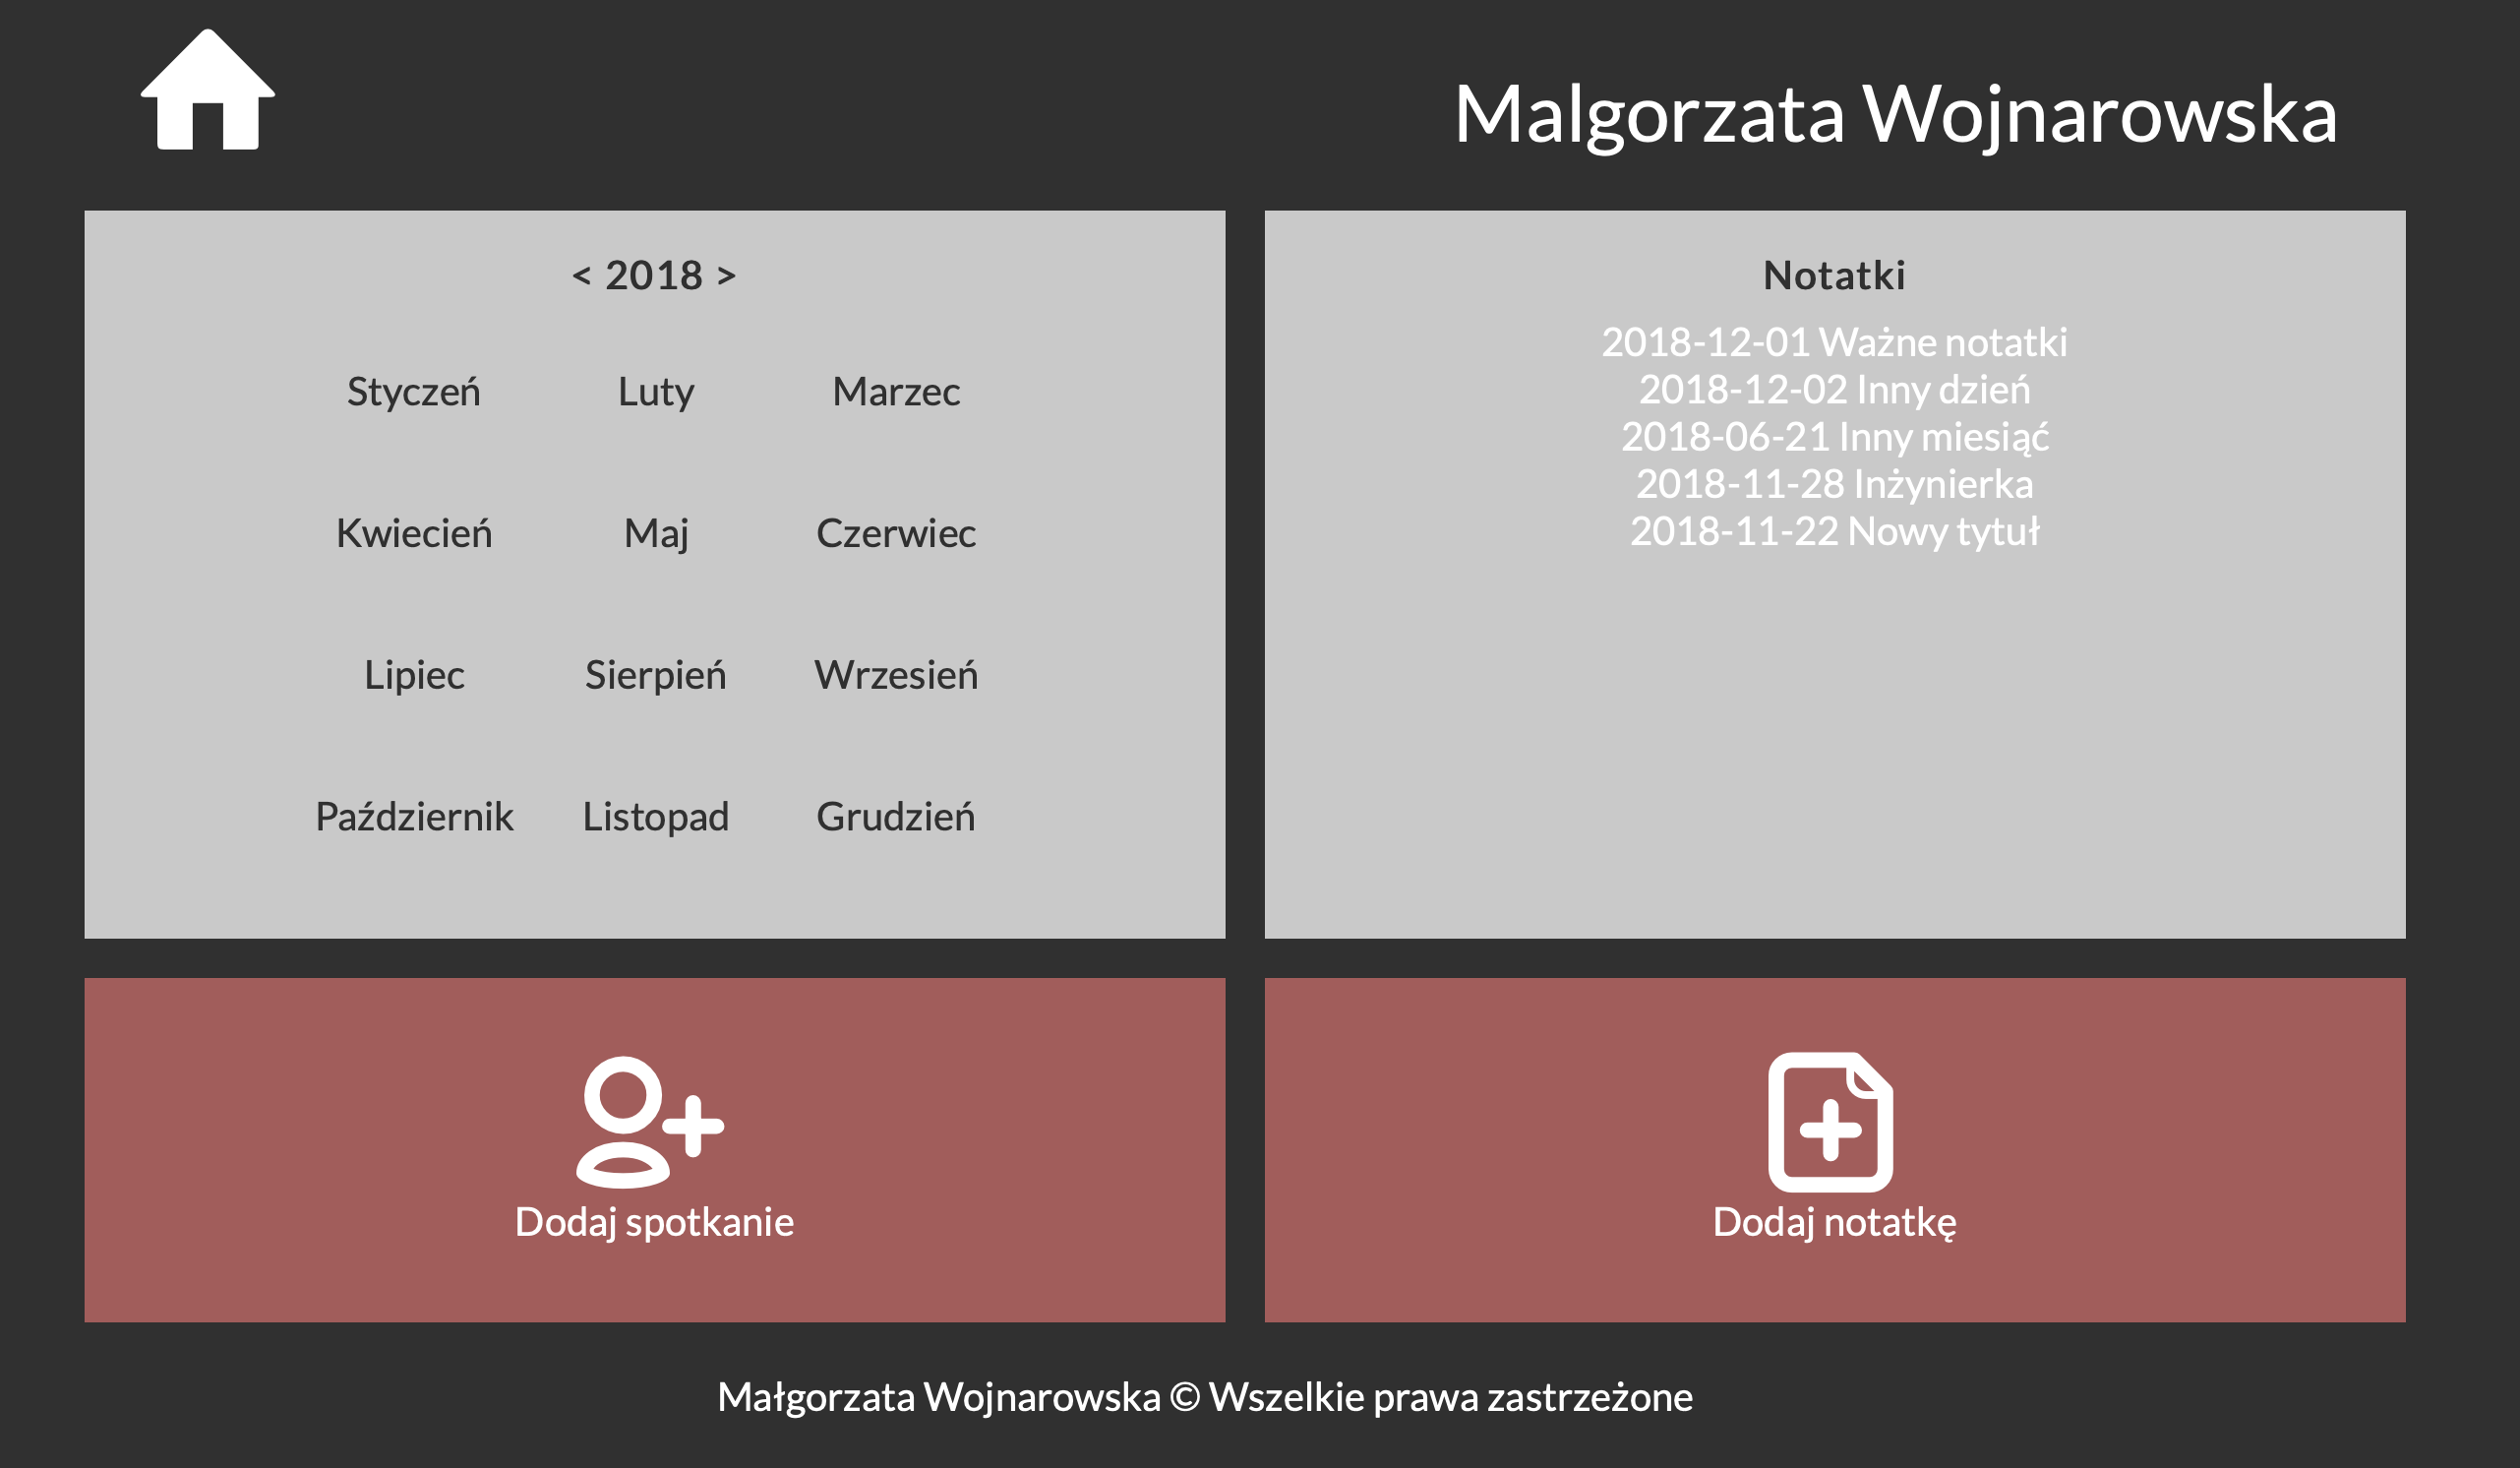
\includegraphics[width=0.75\textwidth]{rok}
		\caption{Widok bieżącego roku}
		\label{fig:23}
	\end{figure}



\section{Wybrane funkcje - opis programowania}

\subsection{Implementacja dostępu do bazy danych}

Do nawiązania połączenia z bazą danych należy wykorzystać rozszerzenie PHP o nazwie MySQLi używając następujących argumentów: (nazwa serwera mysql, login administratora bazy danych, hasło, nazwa bazy danych, z którą nawiązujemy połączenie). Połączenie z bazą danych przedstawione jest na Listingu \ref{lis:14}. Dane te są zapisane w pliku 'connect.php' (Listing \ref{lis:15}).




\begin{lstlisting}[caption={Połączenie z bazą danych}, language=PHP, label={lis:14}]
require_once "connect.php";
mysqli_report(MYSQLI_REPORT_STRICT);
try{      
	$polaczenie = new mysqli($host, $db_user, $db_password, $db_name);
      	if($polaczenie->connect_errno!=0){
        		throw new Exception(mysqli_connect_errno());
      	}
      	else{
      	%make code
	$polaczenie->close();
     	}
}
catch(Exception $e){
      echo 'Error!';
}
\end{lstlisting}







\newpage




	
	
	
\begin{lstlisting}[caption={Wnętrze pliku 'connect.php'}, language=PHP, label={lis:15}]
$host = "localhost";
$db_user = "root";
$db_password = "";
$db_name = "aplikacja";
\end{lstlisting}

	
	

Do odczytania i edycji rekordów w bazie danych, należy użyć kolejnej funkcji oraz podać wybrane zapytanie SQL. Przykłady zapytań przedstawione są na Listingach \ref{lis:16} - \ref{lis:18}.


\begin{lstlisting}[caption={Wybranie klientów o danym adresie e-mail (zapytanie SQL)}, language=PHP, label={lis:16}]
$rezultat = $polaczenie->query("SELECT IdKlienta FROM Klienci WHERE Email='$email'");
\end{lstlisting}

	
\begin{lstlisting}[caption={Dodanie klienta do bazy danych (zapytanie SQL)}, language=PHP, label={lis:17}]
if($polaczenie->query("INSERT INTO Klienci VALUES(NULL, '$imie', '$nazwisko', '$firma', '$email')")){
	$_SESSION['udanedodanieklienta'] = true;
	header("Location: dodanoklienta.php");
}
\end{lstlisting}
	
	
\begin{lstlisting}[caption={Usunięcie wybranej notatki (zapytanie SQL)}, language=PHP, label={lis:18}]
if($polaczenie->query("DELETE FROM Notatki WHERE IdNotatki='$idnotatki' "))
	$_SESSION['udaneusuniecienotatki'] = true;
\end{lstlisting}

	
	


\subsection{Implementacja wybranych funkcjonalności systemu}

Pobieranie danych z bazy dotyczących notatek oraz spotkań danego pracownika przestawione jest na Listingach \ref{lis:19} oraz \ref{lis:20}. Wygląd dnia dla przykładowego pracownika po wyświetleniu spotkań i notatek na dany dzień znajduje się na Rysunku \ref{fig:24}.

	\begin{figure}[H]
		\centering
		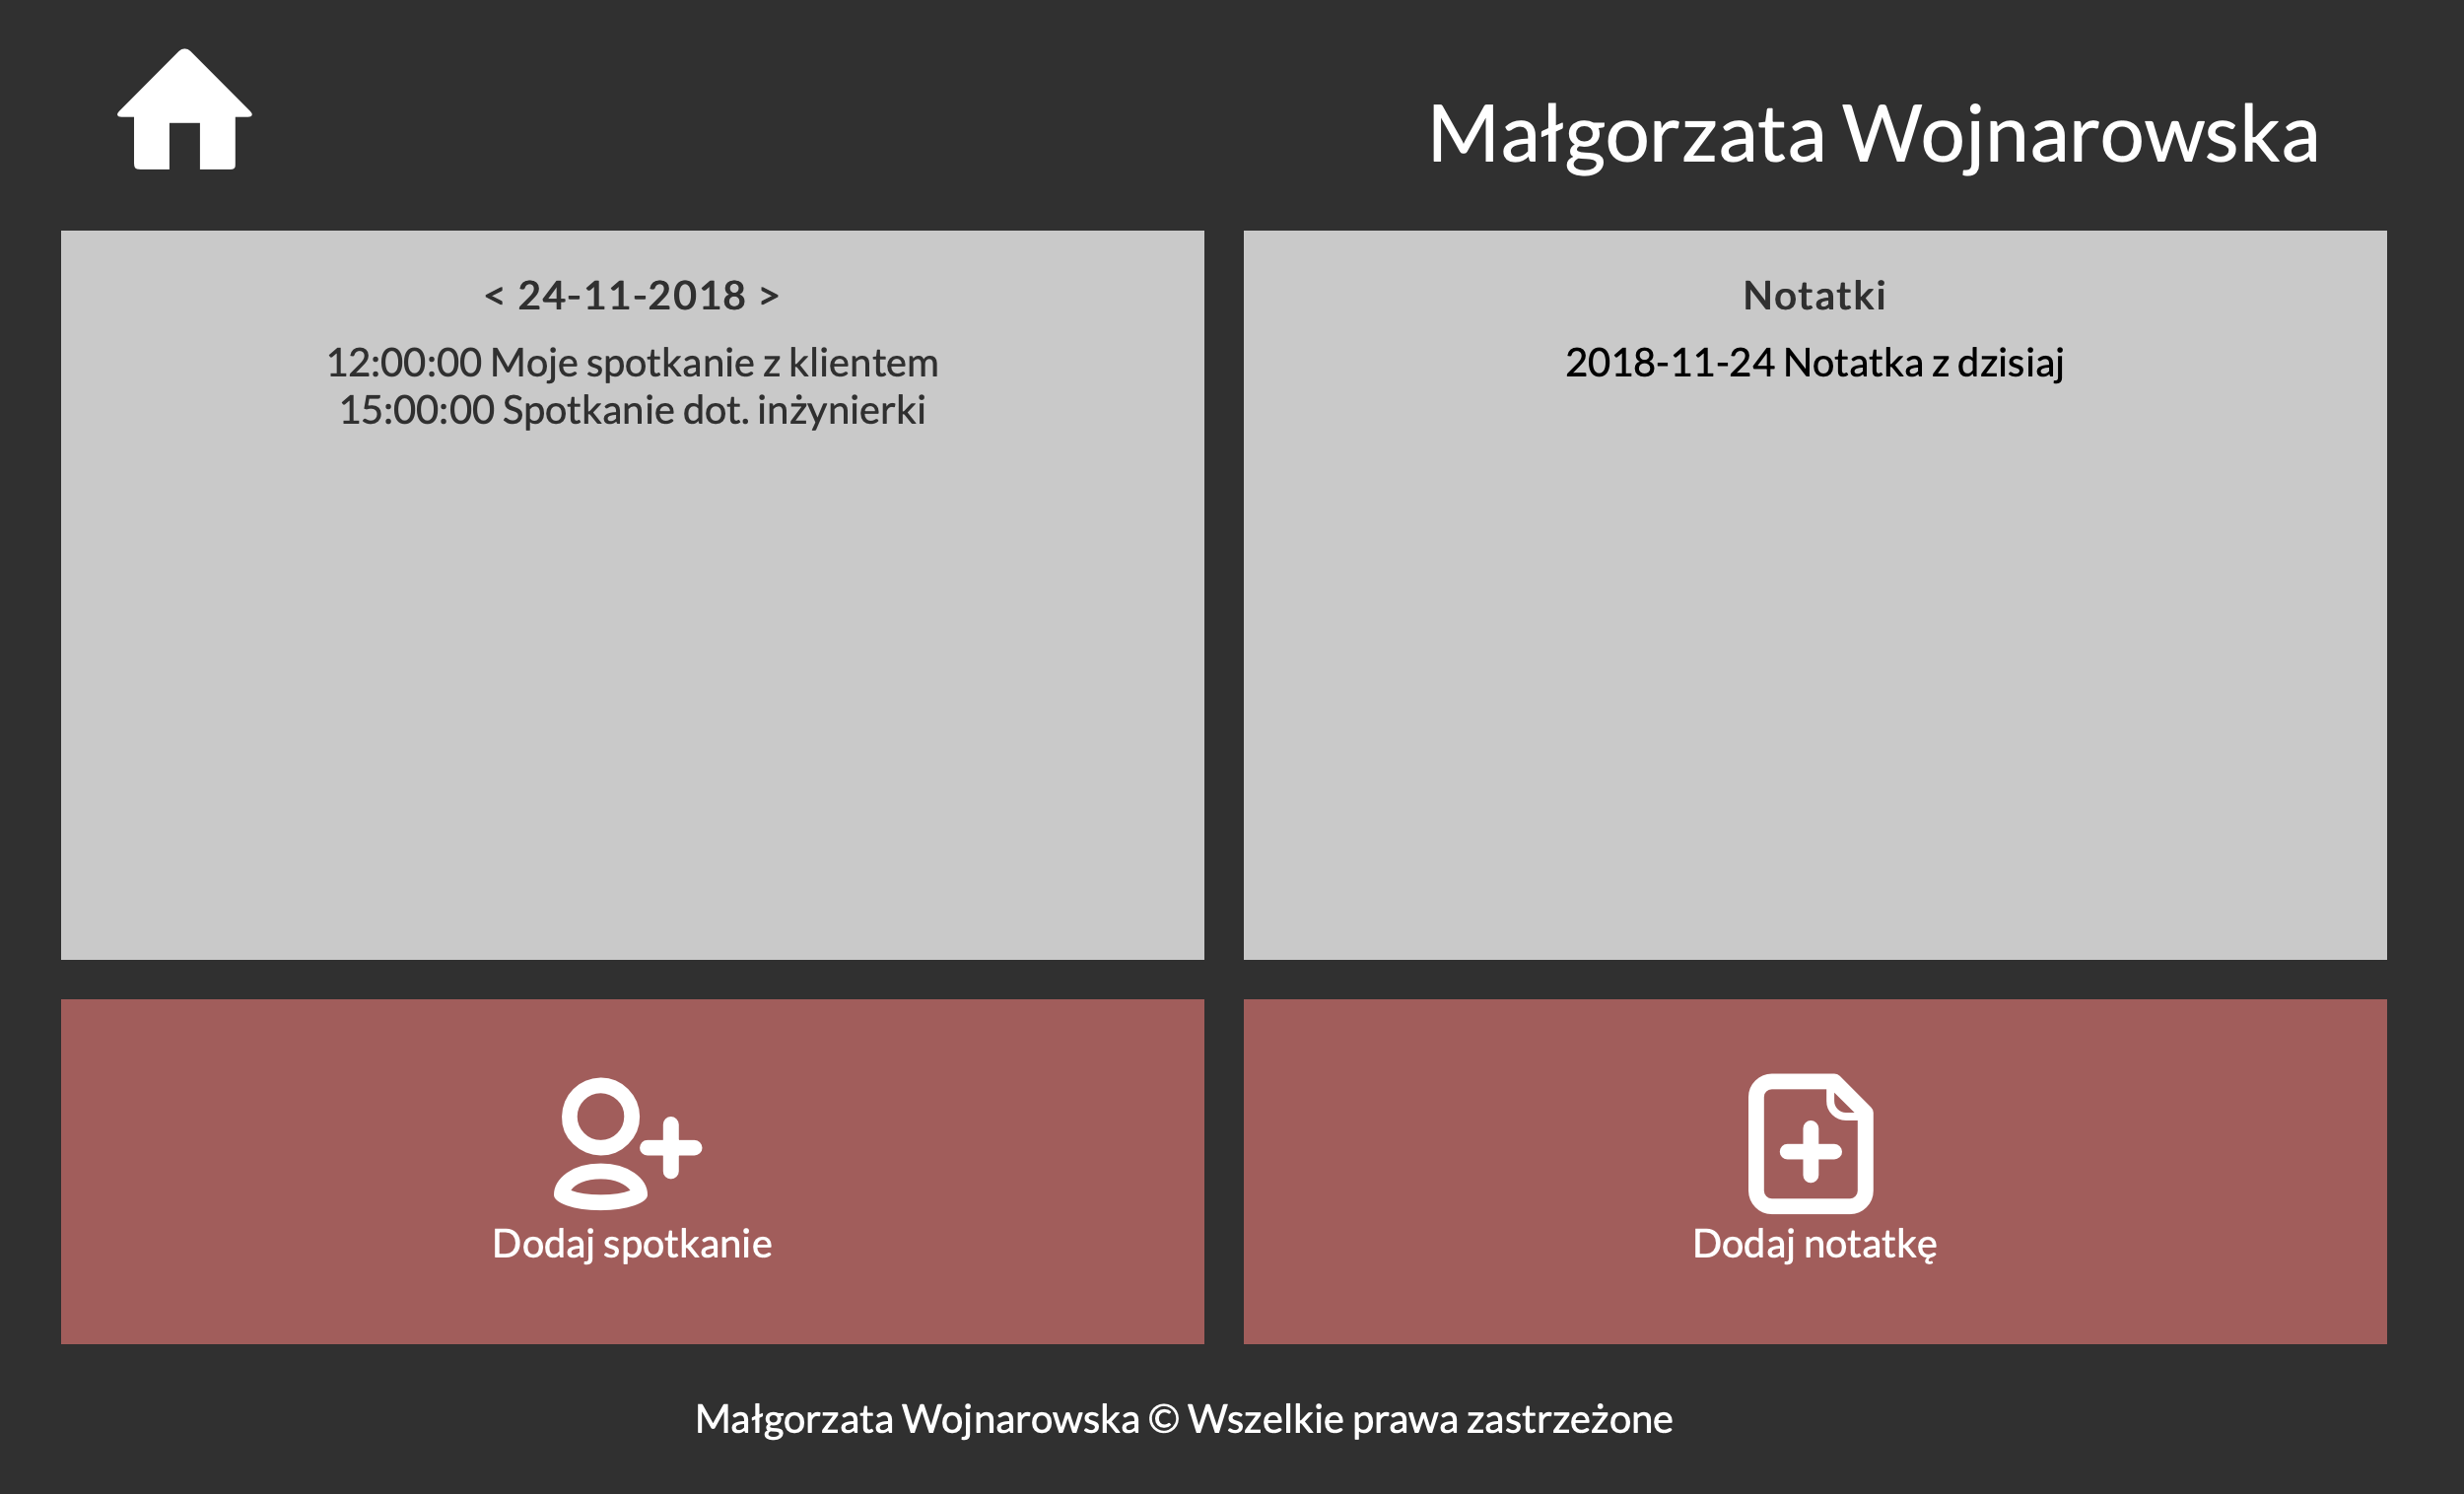
\includegraphics[width=0.75\textwidth]{day}
		\caption{Widok wybranego dnia}
		\label{fig:24}
	\end{figure}
	
	
\begin{lstlisting}[caption={Pobranie spotkań z danego dnia i wyświetlenie ich}, language=PHP, label={lis:19}]
$sql = $polaczenie->query("SELECT * FROM Spotkania WHERE IdPracownika='".$prac['IdPracownika']."' AND MONTH(Data)='".$data->format('m')."' AND DAY(Data)='".$data->format('d')."' AND YEAR(Data)='".$data->format('Y')."'");

while($row = mysqli_fetch_array($sql))
	echo '<a href="dayspotkaniepokaz.php?n1='.$row['IdSpotkania'].'">'.$row['Godzina'].' '.$row['Tytul'].'</a><br/>';
\end{lstlisting}

	
	
	
\begin{lstlisting}[caption={Pobranie notatek z danego dnia i wyświetlenie ich}, language=PHP, label={lis:20}]
$sql = $polaczenie->query("SELECT * FROM Notatki WHERE IdPracownika='".$prac['IdPracownika']."' AND MONTH(Data)='".$data->format('m')."' AND DAY(Data)='".$data->format('d')."' AND YEAR(Data)='".$data->format('Y')."'");
while($row = mysqli_fetch_array($sql))
	echo '<a href="daypokaz.php?n1='.$row['IdNotatki'].'">'.$row['Data'].' '.$row['Tytul'].'</a><br/>';
\end{lstlisting}

	
Przy dacie dnia, miesiąca oraz roku znajdują się strzałki w prawo oraz lewo do przesuwania daty. Przykład po naciśnięciu strzałki dwa razy w prawo (dwa miesiące od dnia bieżącego) przedstawiono na Rysunku \ref{fig:25}. Implementacja tego mechanizmu znajduje się na Listingu \ref{lis:21}.


	
	\begin{figure}[H]
		\centering
		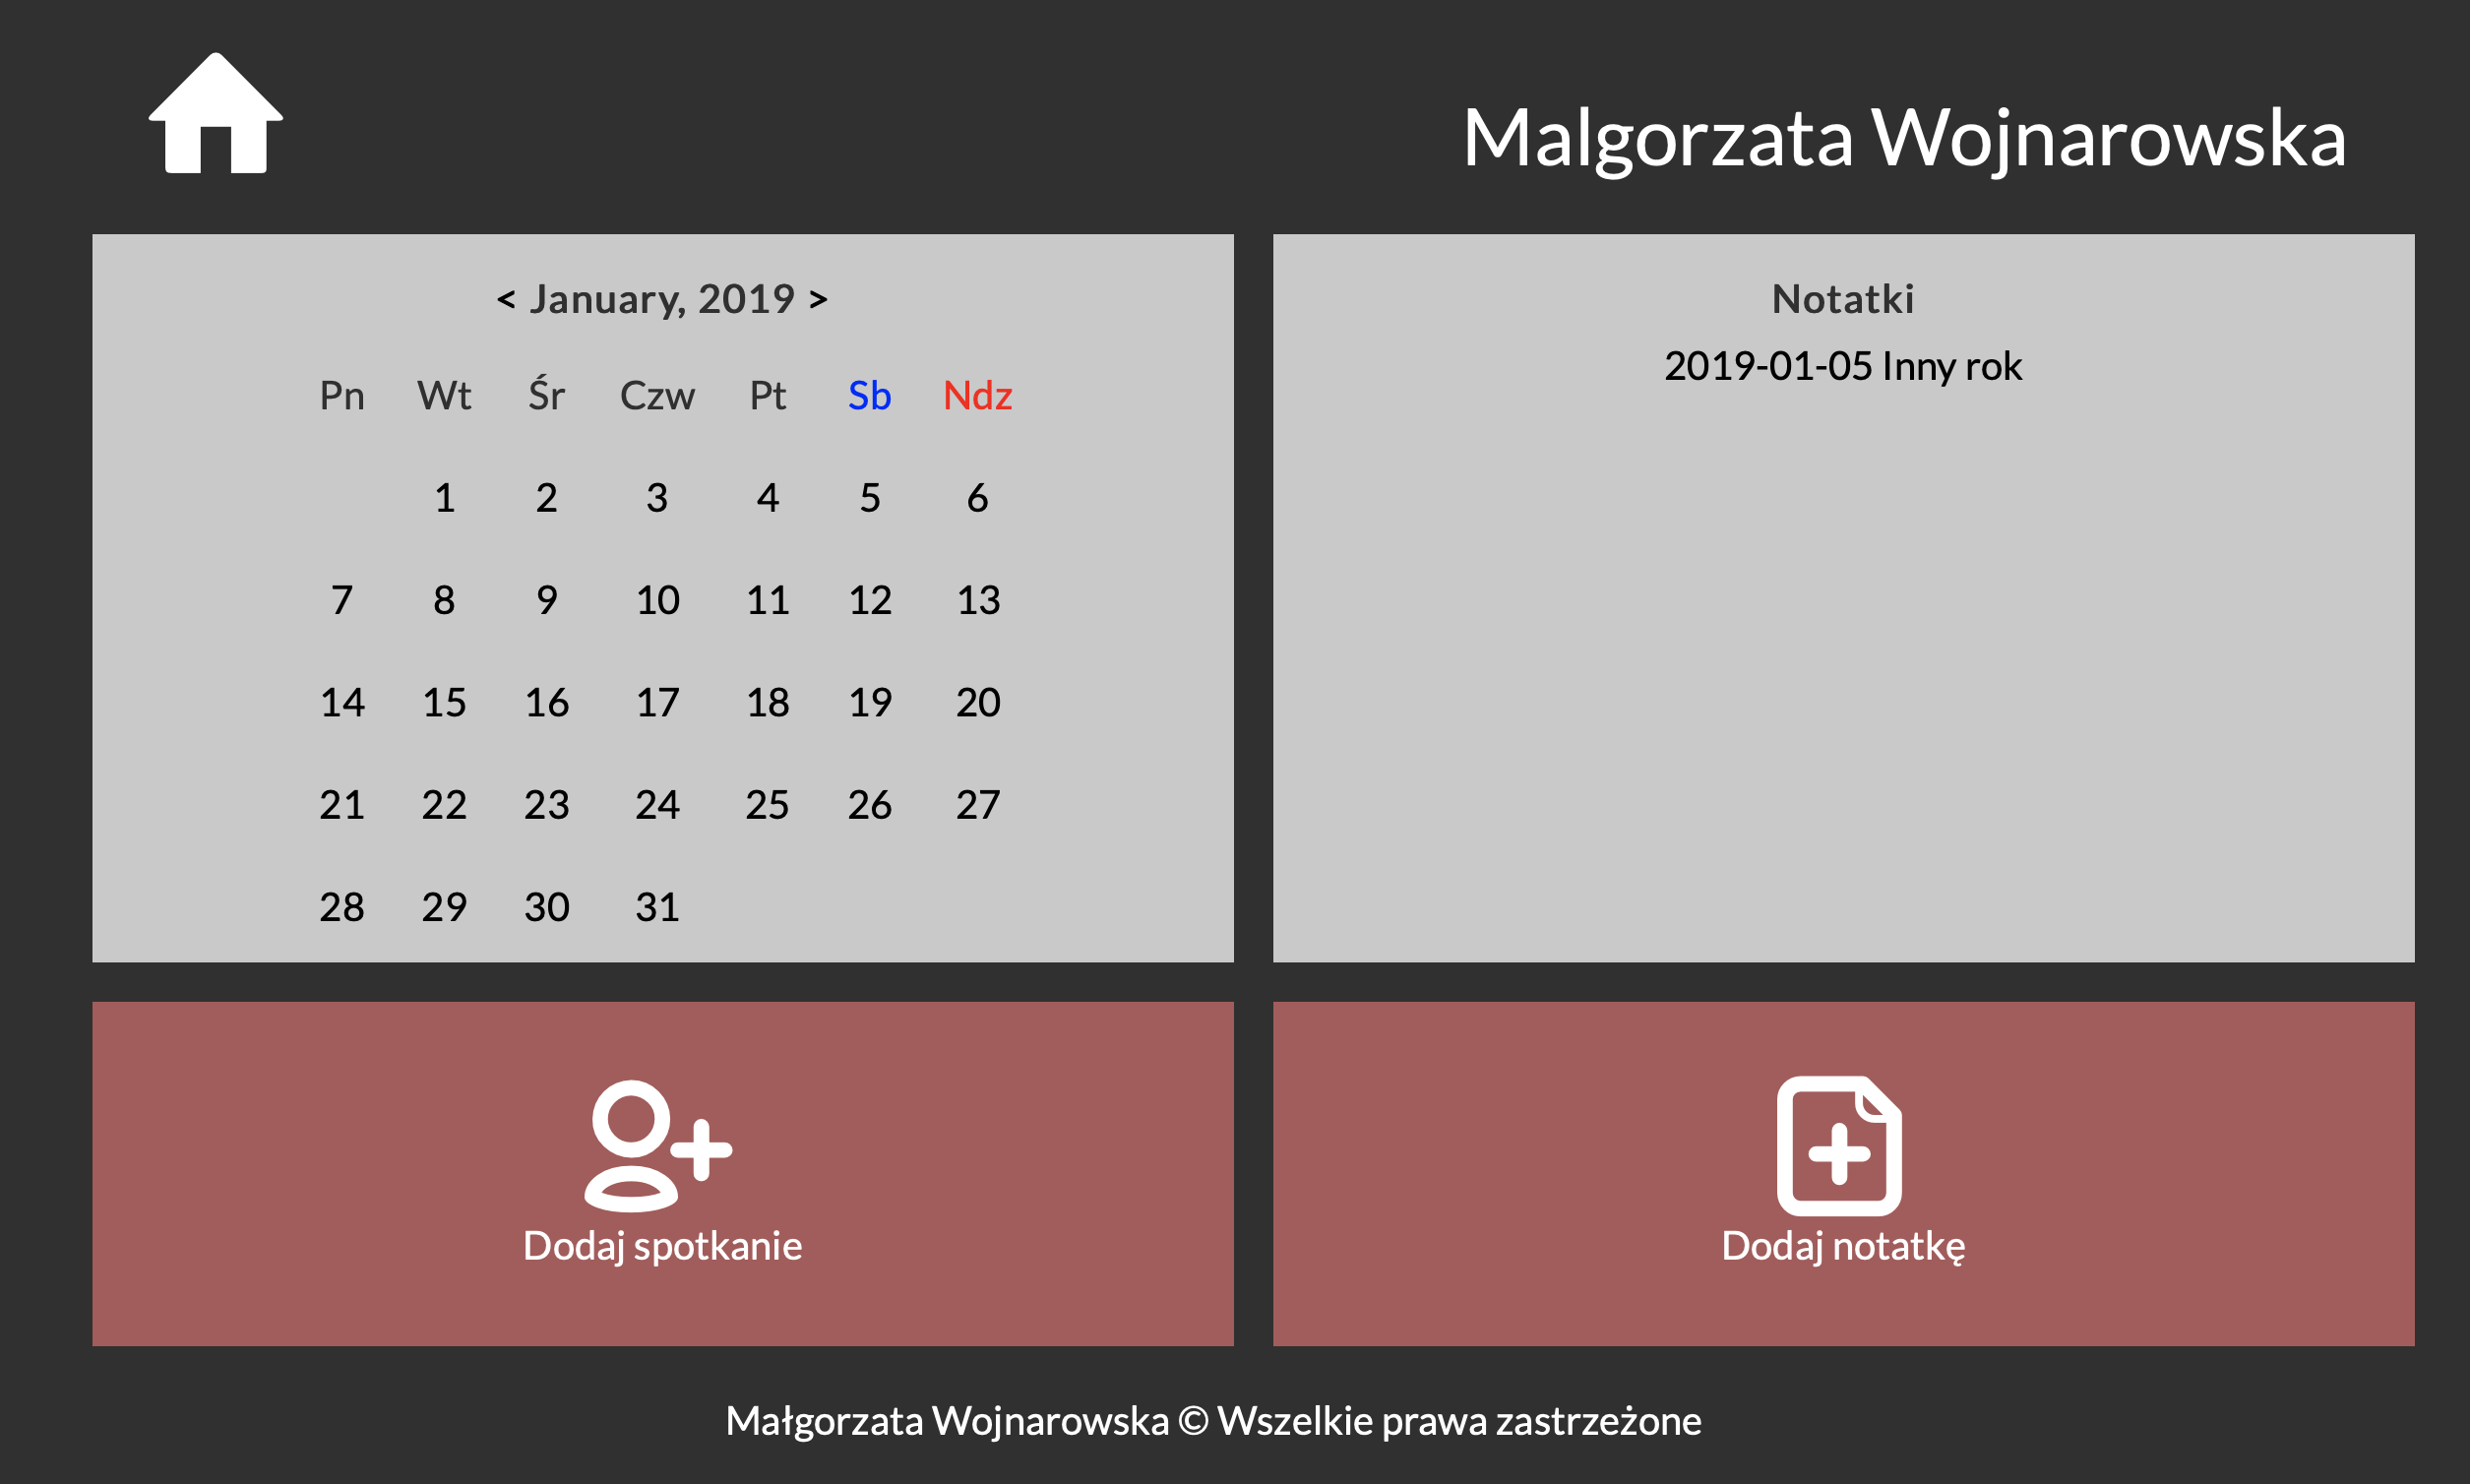
\includegraphics[width=0.75\textwidth]{miesiac_innyrok}
		\caption{Widok po dwukrotnym naciśnięciu strzałki przy nazwie miesiąca w prawo}
		\label{fig:25}
	\end{figure}
	
	\newpage
	
\begin{lstlisting}[caption={Implementacja przesuwania miesiąca}, language=PHP, label={lis:21}]
  $dzisiaj = date('Y-m-j');
  $tytul = date('F, Y', $timestamp);
  $poprzedni = date('Y-m', strtotime('-1 month', $timestamp));
  $nastepny = date('Y-m', strtotime('+1 month', $timestamp));
  //Ilość dni w miesiącu
  $day_count = date('t', $timestamp);
  $str = date('N', $timestamp);
  //Tablica dla kalendarza
  $weeks = [];
  $week = '';
  $week .= str_repeat('<td></td>', $str - 1);
  for ($day = 1; $day <= $day_count; $day++, $str++) {
      $date = $ym . '-' . $day;
      if ($dzisiaj == $date) {
          $week .= '<td class="today">';
      } else {
          $week .= '<td>';
      }
      $y = date('Y', $timestamp);
      $m = date('m', $timestamp);
      $week .= '<a href="month.php?dzien='.$day.'&miesiac='.date('m', $timestamp).'&rok='.date('Y', $timestamp).'&yes=1">' . $day . '</a></td>';
      if ($str % 7 == 0 || $day == $day_count) {
          if ($day == $day_count && $str % 7 != 0) {
              $week .= str_repeat('<td></td>', 7 - $str % 7);
          }
          $weeks[] = '<tr>' . $week . '</tr>';
          $week = '';
      }
  }
\end{lstlisting}

	
		
	

\subsection{Implementacja mechanizmów bezpieczeństwa}

Po naciśnięciu przycisku 'Zaloguj' na stronie głównej, użytkownik zostanie przeniesiony do panelu logowania. Na stronie znajduje się formularz, który należy wypełnić odpowiednimi danymi - loginem użytkownika oraz przypisanym do niego hasłem. Po wpisaniu i zatwierdzeniu danych odbywa się weryfikacja użytkownika oraz sprawdzenie, czy występuje on w bazie danych. Następnie sprawdzana jest poprawność hasła przypisanego do danego konta. Jeśli nie podano danych lub dane te są błędne zostaje wypisany błąd logowania. W przypadku, gdy uwierzytelnienie pracownika zakończyło się pomyślnie zostaje ustawiona zmienna sesyjna 'zalogowany', a pracownik jest przekierowywany do strony 'indexzalogowany', gdzie dostęp mają jedynie zalogowani użytkownicy. Dzięki temu, w prawym górnym rogu pojawia się jego imię i nazwisko. Na Listingu \ref{lis:22} znajduje się implementacja zmiennej sesyjnej.

Sprawdzenie zmiennej sesyjnej jest w każdym pliku oprócz logowania i rejestracji, dlatego próba dostępu do części dla zalogowanych użytkowników zostanie za każdym razem przekierowana do panelu logowania. Będzie ona wznawiała sesję rozpoczętą podczas logowania, dopóki pracownik nie naciśnie przycisku 'Wyloguj', który wyzeruje zmienną 'zalogowany'.

Przy logowaniu hasło ma typ 'password', dzięki czemu nikt nie podejrzy hasła, które jest wpisywane podczas logowania.
	
	
	
\begin{lstlisting}[caption={Zmienna sesyjna - sprawdzenie}, language=PHP, label={lis:22}]
session_start();

if(!isset($_SESSION['zalogowany'])){
	header('Location: logowanie.php');
	exit();
}
\end{lstlisting}

	
	
	
	
	


Jeśli użytkownik nie posiada konta, może się zarejestrować będąc na stronie logowania. W formularzu należy podać imię, nazwisko, stanowisko, email, login oraz hasło, a także zaakceptować regulamin. Wszystkie dane muszą być poprawnie wypełnione, a następnie zostaną przesłane do bazy do tabeli 'Pracownicy'. Implementacja formularza przedstawiona jest na Listingu \ref{lis:23}.

Z uwagi na bezpieczeństwo formularz jest tak zaprojektowany, aby nie można było wykonać ataku komputerowego zwanego 'SQL injection' - czyli metody polegającej na wykorzystaniu luki w zabezpieczeniach polegającej na znajomości zapytań do bazy danych. Dzięki tym zabezpieczeniom nikt nie może się dostać na cudze konto dzięki znajomości zapytań SQL. 









%\newpage





	
\begin{lstlisting}[caption={Implementacja formularza do rejestracji pracownika}, language=HTML, label={lis:23}]
<div class="rectangle" style="width: 1180px; margin: 10px;">
      <form method="post">
        <div class="square2">
            Imię<br/><input type="text" name="imie">
            <br/>Nazwisko<br/><input type="text" name="nazwisko">
            <br/>Stanowisko<br/><input type="text" name="stanowisko">
            <br/>Login<br/><input type="text" name="login">
            <?php
              if(isset($_SESSION['e_login'])){
                echo '<div class="error">'.$_SESSION['e_login'].'</div>';
                unset($_SESSION['e_login']);
              } ?>
        </div>
        <div class="square2">
            Adres e-mail<br/><input type="text" name="email">
            <?php
              if(isset($_SESSION['e_email'])){
                echo '<div class="error">'.$_SESSION['e_email'].'</div>';
                unset($_SESSION['e_email']);
              } ?>
            <br/>Hasło<br/><input type="password" name="haslo">
            <br/>Powtórz hasło<br/><input type="password" name="haslo2">
            <?php
              if(isset($_SESSION['e_haslo'])){
                echo '<div class="error">'.$_SESSION['e_haslo'].'</div>';
                unset($_SESSION['e_haslo']);
              } ?>
            <br/><label><input type="checkbox" name="regulamin"/> Akceptuje regulamin</label>
            <?php
              if(isset($_SESSION['e_regulamin'])){
                echo '<div class="error">'.$_SESSION['e_regulamin'].'</div>';
                unset($_SESSION['e_regulamin']);
              } ?>
        </div>
        <div style="clear:both"></div>
        <button type="submit" class="tile11">
            <i class="icon-meeting"></i>
            <br/>Zarejestruj sie
        </button>
      </form>
    </div>
\end{lstlisting}

	
	
	
	
	
	
	
%\newpage






	
Jednym z takich sposobów jest zabezpieczenie loginu, aby nie mogło w nich być żadnych znaków specjalnych ani polskich znaków, a także kontrolowanie jego długości. Implementacja sprawdzenia poprawności loginu znajduje się na Listingu \ref{lis:24}.

Ponieważ login musi być unikalny sprawdzamy też, czy nie znajduje się już taki w bazie danych (Listing \ref{lis:25}).
	
	

\begin{lstlisting}[caption={Implementacja sprawdzenia poprawności loginu}, language=PHP, label={lis:24}]
//Poprawność loginu
$login = $_POST['login'];
//Sprawdzenie dlugosci loginu
if(strlen($login)<3 || strlen($login)>20){
	$wszystko_ok = false;
	$_SESSION['e_login'] = "Login musi mieć od 3 do 20 znaków!";
}
//login bez znakow polskich, tylko alfanumeryczne
if(!ctype_alnum($login)){
	$wszystko_ok = false;
	$_SESSION['e_login'] = "Login moze skladać się tylko z liter i cyfr, bez polskich znaków!";
}
\end{lstlisting}
		

	
\begin{lstlisting}[caption={Implementacja sprawdzenia czy login istnieje w bazie danych}, language=PHP, label={lis:25}]
//czy login już istnieje
$rezultat = $polaczenie->query("SELECT IdPracownika FROM Pracownicy WHERE Login='$login'");

if(!$rezultat) throw new Exception($polaczenie->error);

if($rezultat->num_rows > 0){
	$wszystko_ok = false;
	$_SESSION['e_login'] = "Istnieje już konto z takim loginem!";
}
\end{lstlisting}
	

	
	







	
Kolejnym zabezpieczeniem jest forma adresu e-mail, korzystamy tu z gotowej funkcji PHP (filter\_var) , dzięki czemu eliminujemy podejrzane znaki z podanego adresu e-mail, a następnie porównujemy czy jest taki sam, jak wpisany. Dzięki temu wiemy, czy takie znaki zostały użyte (Listing \ref{lis:26}).

Tutaj również sprawdzamy unikalność e-maila. Za jego pomocą również możemy się zalogować, dlatego tylko jeden e-mail może być przypisany do jednego konta (Listing \ref{lis:27}).


	
	
\begin{lstlisting}[caption={Implementacja sprawdzenia poprawności e-maila}, language=PHP, label={lis:26}]
//Poprawnosc email
$email = $_POST['email'];
$email_safe = filter_var($email, FILTER_SANITIZE_EMAIL);
if(!filter_var($email_safe, FILTER_VALIDATE_EMAIL) || $email_safe != $email){
	$wszystko_ok = false;
      	$_SESSION['e_email'] = "Podaj poprawny adres e-mail";
}
\end{lstlisting}
	
	
\begin{lstlisting}[caption={Implementacja sprawdzenia czy e-mail istnieje w bazie danych}, language=PHP]
//czy email istnieje
$rezultat = $polaczenie->query("SELECT IdPracownika FROM Pracownicy WHERE Email='$email'");

if(!$rezultat) throw new Exception($polaczenie->error);

if($rezultat->num_rows > 0){
	$wszystko_ok = false;
	$_SESSION['e_email'] = "Istnieje już konto z takim adresem e-mail!";
}
\end{lstlisting}
	

	
	

	
		
	
	
	





	
W przypadku hasła musimy sprawdzić, czy ma ono określoną liczbę znaków, u nas od 3 do 20. Oprócz tego, ponieważ pracownik musi potwierdzić hasło i wpisać je dwa razy - trzeba sprawdzić, czy podane hasła są takie same. W zależności od tego, jaki jest błąd - system wyświetli odpowiedni komunikat, tak jak w poprzednich przypadkach. Na Listingu \ref{lis:27} znajduje się implementacja sprawdzenia poprawności wpisanego hasła.
	
	
	
	
\begin{lstlisting}[caption={Implementacja sprawdzenia poprawności hasła}, language=PHP, label={lis:27}]
//Poprawność hasła
$haslo = $_POST['haslo'];
$haslo2 = $_POST['haslo2'];
//Długość hasła
if(strlen($login)<3 || strlen($login)>20){
	$wszystko_ok = false;
      	$_SESSION['e_haslo'] = "Hasło musi mieć od 3 do 20 znaków!";
}
//Identyczne hasła
if($haslo != $haslo2){
	$wszystko_ok = false;
      	$_SESSION['e_haslo'] = "Podane hasła nie są identyczne!";
}
\end{lstlisting}	
	
	
	
Dla bezpieczeństwa zostało także użyte haszowanie haseł pracowników (Listing \ref{lis:28}), aby nikt nie miał do nich bezpośredniego dostępu - w tym administrator. Dzięki temu, nawet po włamaniu do bazy danych, nikt nie odkryje haseł pracowników. W formularzu zmienna 'haslo' jest także ustawiona jako 'password', dzięki czemu przy wpisywaniu widoczne są jedynie kropki (nikt nie podejrzy hasła przy wpisywaniu). Taka zmienna występuje również przy logowaniu. Zahaszowane hasła w tabeli 'Pracownicy' przedstawione są na Tabeli \ref{tab:9}.
	
	
\begin{lstlisting}[caption={Haszowanie hasła}, language=PHP, label={lis:28}]
$haslo_hash = password_hash($haslo, PASSWORD_DEFAULT);
\end{lstlisting}
	
	
	
	
	\begin{table}[H]
		\centering
		\caption{Zahaszowane hasła w tabeli 'Pracownicy'}
		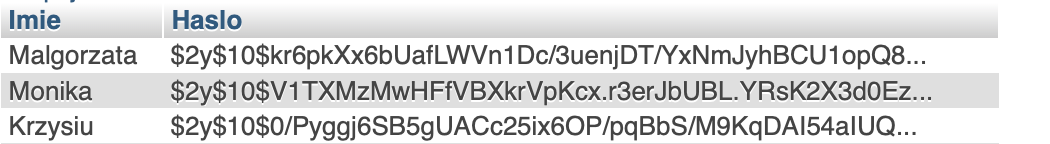
\includegraphics[width=1\textwidth]{haszowanie_tabela}
		\label{tab:9}
	\end{table}
	
	
	

	
	

	
Ostatnim elementem bezpieczeństwa przy rejestracji jest akceptacja regulaminu. Dzięki temu eliminujemy konta tworzone przez sztuczne algorytmy, a także sprawdzamy, że dany użytkownik zgadza się na akceptację naszego regulaminu. Bez zaznaczenia tego checkboxa rejestracja nie zostanie ukończona. Implementacja akceptacji regulaminu znajduje się na Listingu \ref{lis:29}.
	

	
\begin{lstlisting}[caption={Implementacja sprawdzenia czy regulamin został zaakceptowany}, language=PHP, label={lis:29}]
if(!isset($_POST['regulamin'])){
	$wszystko_ok = false;
    	$_SESSION['e_regulamin'] = "Zaakceptuj regulamin!";
}
\end{lstlisting}
	
		
	
	
	
\chapter{Podsumowanie}

Stworzony system jest intuicyjny w użytkowaniu, a także posiada wszystkie zaplanowane funkcjonalności. Aplikacja ma estetyczny i prosty wygląd kafelkowy, który sprawia, że poruszanie się po niej jest proste i przyjemne. Dzięki planowaniu spotkań oraz tworzeniu notatek można w łatwy sposób zorganizować codzienny grafik. Dzięki notatkom, które można przypisywać do konkretnej daty, można mieć zapisane ważne rzeczy do zrobienia danego dnia, które niekoniecznie powiązane są ze spotkaniami.

Aplikacja została wykonana zgodnie z ustalonymi założeniami. Projekt spełnia postawione wymagania oraz przeszedł pozytywnie zaplanowane testy, które miały na celu sprawdzić poprawność działania aplikacji do planowania systemów biznesowych. Zaimplementowane funkcje działają zgodnie z oczekiwaniami, w tym planowania spotkań oraz notatek, a także zarządzanie nimi. Wybrane zabezpieczenia zarówno na poziomie relacyjnej bazy danych, a także aplikacji spełniają swoją rolę. Poprawność działania aplikacji, bazy danych oraz ich połączenia zostały sprawdzone przy pomocy testów, których wynik jest pozytywny.

System w przyszłości można rozwinąć tak, aby był maksymalnie funkcjonalny dla pracowników firmy. Można by poszerzyć uprawnienia prezesa firmy, który mógłby dodawać spotkania swoim pracownikom, a także pozwolić jego asystentce na planowanie spotkań prezesowi. Można także wyłączyć opcję rejestracji, a stworzyć dodawanie pracowników jedynie przez uprawnione osoby z kadr. Dzięki temu aplikacja byłaby jeszcze bardziej spersonalizowana do użytku dla firm. System mógłby także wysyłać powiadomienie na e-mail klienta, które poinformuje go o tym, że ktoś rzeczywiście zaplanował z nim spotkanie na konkretny dzień i godzinę. 

System ma duże możliwości rozwoju, ale już teraz jest wystarczająco funkcjonalny, aby znacznie ułatwić i przyśpieszyć planowanie spotkań biznesowych. 

\begin{thebibliography}{9}
  
  \bibitem{bib:1}
  Welling Luke, Thomson Laura,
  \emph{PHP i MySQL. Tworzenie stron WWW. Vademecum profesjonalisty}.
  Helion, Gliwice,
  Wydanie czwarte,
  2009.
  
  \bibitem{bib:2}
  Lis Marcin,
  \emph{PHP i MySQL. Dla każdego}.
  Helion, Gliwice,
  Wydanie trzecie,
  2017.
  
  \bibitem{bib:3}
  Duckett Jon,
  \emph{HTML i CSS. Zaprojektuj i zbuduj witrynę WWW}.
  Helion, Gliwice,
  2014
  
  \begin{comment}
  ZESZYTY NAUKOWE MA£OPOLSKIEJ WY ̄SZEJ SZKO£Y EKONOMICZNEJ W TARNOWIE NR 2(13)/2009 T. 2
  LESZEK KOZIO£, RADOS£AW PYREK*
  Model systemu zarz1dzania czasem pracy w przedsiêbiorstwie  
  
  C z e k a j J. 2008. Wzorce przebiegu przedsięwzięć a koszty czasu. W: Stabryła A. (red.). Zarządzanie rozwojem organizacji w społeczeństwie informacyjnym. Studia i Prace UEK. Kraków: Uniwersytet Ekonomiczny.
  
  K o z i o ł L. 1991. Uwarunkowania efektywnego wykorzystania czasu pracy w przemyśle. „Zeszyty Na- ukowe Seria Specjalna: Monografie” nr 101. Kraków: Akademia Ekonomiczna.
  \end{comment}
  
\end{thebibliography}



\addcontentsline{toc}{chapter}{Bibliografia} %utworzenie w spisie treści pozycji Bibliografia
\bibliography{bibliografia} % wstawia bibliografię korzystając z pliku bibliografia.bib - dotyczy BibTeXa, jeżeli nie korzystamy z BibTeXa należy użyć otoczenia thebibliography

%opcjonalnie może się tu pojawić spis rysunków i tabel
 \listoffigures
 \lstlistoflistings
 \listoftables
 
 \end{document}
